% (unofficial) La Trobe PhD Thesis Template
% Copyright (C) 2018 Matthias Langer
%
% This program is free software; you can redistribute it and/or modify
% it under the terms of the GNU General Public License as published by
% the Free Software Foundation; either version 2 of the License, or
% (at your option) any later version.
%
% This program is distributed in the hope that it will be useful,
% but WITHOUT ANY WARRANTY; without even the implied warranty of
% MERCHANTABILITY or FITNESS FOR A PARTICULAR PURPOSE.  See the
% GNU General Public License for more details.
%
% You should have received a copy of the GNU General Public License along
% with this program; if not, write to the Free Software Foundation, Inc.,
% 51 Franklin Street, Fifth Floor, Boston, MA 02110-1301 USA.
%
\RequirePackage[english=usenglishmax]{hyphsubst}
\documentclass[twoside,openright,titlepage,numbers=noenddot,headinclude,footinclude=true,cleardoublepage=empty,listof=totoc,paper=a4,fontsize=11pt,australian,twoside=semi,DIV=calc]{scrreprt} 

% -----------------------------------------------------------------------------
%   CONFIGURATION
% -----------------------------------------------------------------------------
% Thesis and submission:
\newcommand{\myTitle}{An intelligent system approach for Industrial data forecasting: WWTP as a case of study}
\newcommand{\mySubmissionYear}{2021}
\newcommand{\mySubmissionMonth}{November}
\newcommand{\mySubmissionDay}{30}

% Regarding yourself:
\newcommand{\myFirstName}{Carlos Andres}
\newcommand{\myLastName}{Cárdenas Pérez}
\newcommand{\myWebsite}{}
\newcommand{\myBirthYear}{1997}
\newcommand{\myBirthMonth}{September}
\newcommand{\myBirthDay}{30}
\newcommand{\myBirthPlace}{Colombia}

% Primary supervisor:
\newcommand{\myProfTitle}{Ph.D.}
\newcommand{\myProfFirstName}{Christian G.}
\newcommand{\myProfLastName}{Quintero M. }
\newcommand{\myProfWebsite}{}

% Co-supervisor:
\newcommand{\myOtherProfTitle}{}
\newcommand{\myOtherProfFirstName}{}
\newcommand{\myOtherProfLastName}{}
\newcommand{\myOtherProfWebsite}{}

% University related:
\newcommand{\myDepartment}{Department of Electrical and Electronic Engineering}
\newcommand{\myFaculty}{}
\newcommand{\mySchool}{}
\newcommand{\myUni}{Universidad del Norte}
% -----------------------------------------------------------------------------

% ****************************************************************************************************
% classicthesis-config.tex 
% formerly known as loadpackages.sty, classicthesis-ldpkg.sty, and classicthesis-preamble.sty 
% Use it at the beginning of your ClassicThesis.tex, or as a LaTeX Preamble 
% in your ClassicThesis.{tex,lyx} with % ****************************************************************************************************
% classicthesis-config.tex 
% formerly known as loadpackages.sty, classicthesis-ldpkg.sty, and classicthesis-preamble.sty 
% Use it at the beginning of your ClassicThesis.tex, or as a LaTeX Preamble 
% in your ClassicThesis.{tex,lyx} with % ****************************************************************************************************
% classicthesis-config.tex 
% formerly known as loadpackages.sty, classicthesis-ldpkg.sty, and classicthesis-preamble.sty 
% Use it at the beginning of your ClassicThesis.tex, or as a LaTeX Preamble 
% in your ClassicThesis.{tex,lyx} with \input{classicthesis-config}
% ****************************************************************************************************  
% If you like the classicthesis, then I would appreciate a postcard. 
% My address can be found in the file ClassicThesis.pdf. A collection 
% of the postcards I received so far is available online at 
% http://postcards.miede.de
% ****************************************************************************************************
% !!! ATTENTION !!! ATTENTION !!! ATTENTION !!! ATTENTION !!!
% This version was modified to comply with the formatting guidelines
% of the Graduate Research School of La Trobe University.
% ~ October 2018 / Matthias Langer (https://github.com/bashimao/ltu-thesis)
% !!! ATTENTION !!! ATTENTION !!! ATTENTION !!! ATTENTION !!!
% ****************************************************************************************************


% ****************************************************************************************************
% 0. Set the encoding of your files. UTF-8 is the only sensible encoding nowadays. If you can't read
% äöüßáéçèê∂åëæƒÏ€ then change the encoding setting in your editor, not the line below. If your editor
% does not support utf8 use another editor!
% ****************************************************************************************************
\PassOptionsToPackage{utf8}{inputenc}
	\usepackage{inputenc}


% ****************************************************************************************************
% 1. Configure classicthesis for your needs here, e.g., remove "drafting" below 
% in order to deactivate the time-stamp on the pages
% ****************************************************************************************************
\PassOptionsToPackage{eulerchapternumbers,listings,pdfspacing,beramono,dottedtoc}{classicthesis}
% ********************************************************************
% Available options for classicthesis.sty 
% (see ClassicThesis.pdf for more information):
% drafting
% parts nochapters linedheaders
% eulerchapternumbers beramono eulermath pdfspacing minionprospacing
% tocaligned dottedtoc manychapters
% listings floatperchapter subfig
% ********************************************************************


% ****************************************************************************************************
% 2. Personal data and user ad-hoc commands
% ****************************************************************************************************
% moved to thesis.tex


% ********************************************************************
% Setup, finetuning, and useful commands
% ********************************************************************
\newcounter{dummy} % necessary for correct hyperlinks (to index, bib, etc.)
\newlength{\abcd} % for ab..z string length calculation
\providecommand{\mLyX}{L\kern-.1667em\lower.25em\hbox{Y}\kern-.125emX\@}
\newcommand{\ie}{i.\,e.\ }
\newcommand{\Ie}{I.\,e.\ }
\newcommand{\eg}{e.\,g.\ }
\newcommand{\Eg}{E.\,g.\ }
\newcommand{\fig}[1]{{Fig.~\ref{#1}}}
% ****************************************************************************************************


% ****************************************************************************************************
% 3. Loading some handy packages
% ****************************************************************************************************
% ******************************************************************** 
% Packages with options that might require adjustments
% ******************************************************************** 
\PassOptionsToPackage{australian}{babel}
  \usepackage{babel}

\usepackage{csquotes}
\PassOptionsToPackage{%
  backend=bibtex,
  bibencoding=ascii,
  language=auto,
  bibstyle=ieee, 	%chem-acs
  citestyle=numeric-comp, % \textbf{}
  sorting=none,
  maxbibnames=10,
  natbib=true
}{biblatex}
  \usepackage{biblatex}

%\PassOptionsToPackage{fleqn}{amsmath}  %Align equations to the left     % math environments and more by the AMS 
  \usepackage{amsmath}

% ******************************************************************** 
% General useful packages
% ******************************************************************** 
\usepackage{amssymb}
\usepackage{gensymb}
\usepackage{lipsum}
\PassOptionsToPackage{T1}{fontenc} % T2A for cyrillics
    \usepackage{fontenc}
\usepackage{textcomp} % fix warning with missing font shapes
\usepackage{scrhack} % fix warnings when using KOMA with listings package  
\usepackage{xspace} % to get the spacing after macros right
\usepackage{mparhack} % get marginpar right
%\usepackage[latest]{latexrelease} % will be used once available in more distributions (ISSUE #107)
\PassOptionsToPackage{printonlyused,smaller}{acronym}
  \usepackage{acronym} % nice macros for handling all acronyms in the thesis
  %\renewcommand{\bflabel}[1]{{#1}\hfill} % fix the list of acronyms --> no longer working
  %\renewcommand*{\acsfont}[1]{\textsc{#1}}
  \renewcommand*{\aclabelfont}[1]{\acsfont{#1}}

\usepackage{afterpage}
\usepackage[version=4]{mhchem}

% ****************************************************************************************************


% ****************************************************************************************************
% 4. Setup floats: tables, (sub)figures, and captions
% ****************************************************************************************************
\usepackage{tabularx} % better tables
\setlength{\extrarowheight}{3pt} % increase table row height
\newcommand{\tableheadline}[1]{\multicolumn{1}{c}{\spacedlowsmallcaps{#1}}}
\newcommand{\myfloatalign}{\centering} % to be used with each float for alignment
\usepackage{makecell}
\usepackage{multirow}
\usepackage{caption}
\usepackage{subcaption}
\usepackage{notoccite} %Removes citations from toc
\usepackage{longtable}%

\usepackage{comment}
\usepackage{pdflscape}
%\usepackage[dvipsname]{xcolor} %For printing 
\usepackage[svgnames]{xcolor} %For PDF
\usepackage{colortbl}%
  \newcommand{\myrowcolour}{\rowcolor[gray]{0.925}}
\usepackage{booktabs}

\newcommand{\cheading}[2]{\textcolor{black}{\textbf{#1\hfill #2}}}


% Thanks to cgnieder and Claus Lahiri
% http://tex.stackexchange.com/questions/69349/spacedlowsmallcaps-in-caption-label
% [REMOVED DUE TO OTHER PROBLEMS, SEE ISSUE #82]    
%\DeclareCaptionLabelFormat{smallcaps}{\bothIfFirst{#1}{~}\MakeTextLowercase{\textsc{#2}}}
%\captionsetup{font=small,labelformat=smallcaps} % format=hang,
\captionsetup{font=small} % format=hang,
%\usepackage{subfig} %Possible Errors when using inconjunction with subcaption

\newcommand*{\figureautorefname}{Fig.}
% ****************************************************************************************************

\usepackage{etoolbox}
\makeatletter
\newif\if@in@acrolist

\AtBeginEnvironment{acronym}{\@in@acrolisttrue}
\newrobustcmd{\LU}[2]{\if@in@acrolist#1\else#2\fi}

\newcommand{\ACF}[1]{{\@in@acrolisttrue\acf{#1}}}
\makeatother

% ****************************************************************************************************
% 5. Setup code listings
% ****************************************************************************************************
\usepackage{listings}
%\lstset{emph={trueIndex,root},emphstyle=\color{BlueViolet}}%\underbar} % For special keywords
\lstset{language=[LaTeX]Tex,%C++,
  morekeywords={PassOptionsToPackage,selectlanguage},
  keywordstyle=\color{RoyalBlue},%\bfseries,
  basicstyle=\small\ttfamily,
  %identifierstyle=\color{NavyBlue},
  commentstyle=\color{Green}\ttfamily,
  stringstyle=\rmfamily,
  numbers=left,
  numberstyle=\scriptsize,%\tiny
  stepnumber=5,
  numbersep=8pt,
  showstringspaces=false,
  breaklines=true,
  %frameround=ftff,
  %frame=single,
  belowcaptionskip=.75\baselineskip
  %frame=L
}
% ****************************************************************************************************             


% ****************************************************************************************************
% 6. PDFLaTeX, hyperreferences and citation backreferences
% ****************************************************************************************************
% ********************************************************************
% Using PDFLaTeX
% ********************************************************************
\PassOptionsToPackage{pdftex,hyperfootnotes=false,pdfpagelabels}{hyperref}
\usepackage{hyperref}  % backref linktocpage pagebackref
\pdfcompresslevel=9
\pdfadjustspacing=1
\PassOptionsToPackage{pdftex}{graphicx}
    \usepackage{graphicx} 


% ********************************************************************
% Hyperreferences
% ********************************************************************
\hypersetup{breaklinks=true}
\hypersetup{linktocpage=true}
\hypersetup{colorlinks=true}
\hypersetup{urlcolor=webbrown}
\hypersetup{linkcolor=RoyalBlue}
\hypersetup{citecolor=webgreen}
\hypersetup{pageanchor=true}
\hypersetup{plainpages=false}
%\hypersetup{bookmarksnumbered=true}
%\hypersetup{bookmarksopen=true}
%\hypersetup{bookmarksopenlevel=true}
%hypertexnames=true, nesting=true, frenchlinks
\hypersetup{pdfstartpage=3}
\hypersetup{pdfstartview=FitV}
\hypersetup{pdfpagemode=UseNone}
\hypersetup{pageanchor=true}
\hypersetup{pdfpagemode=UseOutlines}
\hypersetup{pdftitle={\myTitle}}
\hypersetup{pdfauthor={\textcopyright\ \myFirstName\ \myLastName, \myUni, \myFaculty}}
\hypersetup{pdfsubject={}}
\hypersetup{pdfkeywords={}}
\hypersetup{pdfhighlight=/O}

%********************************************************
%Removes link color for printing by uncommenting, remember to change xcolor to cmyk for officeworks printing
%********************************************************

% \hypersetup{hidelinks} %Removes link colours?


% ********************************************************************
% Setup autoreferences
% ********************************************************************
% There are some issues regarding autorefnames
% http://www.ureader.de/msg/136221647.aspx
% http://www.tex.ac.uk/cgi-bin/texfaq2html?label=latexwords
% you have to redefine the makros for the 
% language you use, e.g., australian, ngerman
% (as chosen when loading babel/AtBeginDocument)
% ********************************************************************
\makeatletter
\@ifpackageloaded{babel}%
{%
  \addto\extrasaustralian{%
    \renewcommand*{\figureautorefname}{Fig.}%
    \renewcommand*{\equationautorefname}{Eqn.}%
    \renewcommand*{\tableautorefname}{Table}%
    \renewcommand*{\partautorefname}{Part}%
    \renewcommand*{\chapterautorefname}{Chapter}%
    \renewcommand*{\sectionautorefname}{\S}%
    \renewcommand*{\subsectionautorefname}{\S}%
    \renewcommand*{\subsubsectionautorefname}{\S}%
  }%
  \addto\extrasngerman{%
    \renewcommand*{\paragraphautorefname}{Absatz}%
    \renewcommand*{\subparagraphautorefname}{Unterabsatz}%
    \renewcommand*{\footnoteautorefname}{Fu\"snote}%
    \renewcommand*{\FancyVerbLineautorefname}{Zeile}%
    \renewcommand*{\theoremautorefname}{Theorem}%
    \renewcommand*{\appendixautorefname}{Anhang}%
    \renewcommand*{\equationautorefname}{Gleichung}%
    \renewcommand*{\itemautorefname}{Punkt}%
  }%
  % Fix to getting autorefs for subfigures right (thanks to Belinda Vogt for changing the definition)
  \providecommand{\subfigureautorefname}{\figureautorefname}%
}{\relax}
\makeatother


% ****************************************************************************************************
% 7. Last calls before the bar closes
% ****************************************************************************************************
% ********************************************************************
% Development Stuff
% ********************************************************************
%\listfiles
%\PassOptionsToPackage{l2tabu,orthodox,abort}{nag}
%   \usepackage{nag}
%\PassOptionsToPackage{warning, all}{onlyamsmath}
%   \usepackage{onlyamsmath}

% ********************************************************************
% Last, but not least...
% ********************************************************************
\usepackage{classicthesis}
% ****************************************************************************************************


% ****************************************************************************************************
% 8. Further adjustments (experimental)
% ****************************************************************************************************
% ********************************************************************
% Changing the text area
% ********************************************************************
%\linespread{1.05} % a bit more for Palatino
%\areaset[current]{312pt}{761pt} % 686 (factor 2.2) + 33 head + 42 head \the\footskip
%\setlength{\marginparwidth}{7em}%
%\setlength{\marginparsep}{2em}%

% ********************************************************************
% Using different fonts
% ********************************************************************
%\usepackage[oldstylenums]{kpfonts} % oldstyle notextcomp
%\usepackage[osf]{libertine}
%\usepackage[light,condensed,math]{iwona}
%\renewcommand{\sfdefault}{iwona}
%\usepackage{lmodern} % <-- no osf support :-(
%\usepackage{cfr-lm} % 
%\usepackage[urw-garamond]{mathdesign} <-- no osf support :-(
%\usepackage[default,osfigures]{opensans} % scale=0.95 
%\usepackage[sfdefault]{FiraSans}
% ****************************************************************************************************


% ****************************************************************************************************
% 9. LTU Extensions
% ****************************************************************************************************
\usepackage{colortbl}
\usepackage{setspace}
\usepackage{fp}
\usepackage{soul}

\usepackage{textcomp}

\usepackage{pgfplots}
\usepackage{pgfplotstable}
\pgfplotsset{compat=newest}
\usepackage[separate-uncertainty = true,multi-part-units=single]{siunitx}



\sisetup{separate-uncertainty}

\usepackage[shortcuts]{extdash}
%\usepackage{epigraph}

\usepackage{tikz-timing}[2011/01/09]
\usetikzlibrary{arrows, backgrounds, patterns, shapes}
\usepackage{arydshln}

\usepackage{algorithm}
\usepackage{algorithmic}
\newcommand{\algorithmautorefname}{Algorithm}

\renewcommand{\lstlistlistingname}{List of Listings}

\DeclareMathOperator*{\argmin}{argmin}
\DeclareMathOperator*{\argmax}{argmax}

\renewcommand{\rmdefault}{pnc}
\renewcommand{\rmdefault}{pplx}

\newcolumntype{L}[1]{>{\raggedright\arraybackslash}m{#1}}
\newcolumntype{C}[1]{>{\centering\arraybackslash}m{#1}}
\newcolumntype{R}[1]{>{\raggedleft\arraybackslash}m{#1}}

\numberwithin{equation}{chapter}
\numberwithin{figure}{chapter}
\numberwithin{table}{chapter}
\numberwithin{algorithm}{chapter}
\sloppy

\renewcommand{\bibfont}{\footnotesize}

\newcommand{\hinttext}[1]{\textcolor{Gray!70!Red}{#1}}





\renewcommand{\topfraction}{.8}
\renewcommand{\floatpagefraction}{.8}% %reduces the odd a float gets its own page unless it takes up 80% of space

\hyphenation{Vertical}

% ****************************************************************************************************  
% If you like the classicthesis, then I would appreciate a postcard. 
% My address can be found in the file ClassicThesis.pdf. A collection 
% of the postcards I received so far is available online at 
% http://postcards.miede.de
% ****************************************************************************************************
% !!! ATTENTION !!! ATTENTION !!! ATTENTION !!! ATTENTION !!!
% This version was modified to comply with the formatting guidelines
% of the Graduate Research School of La Trobe University.
% ~ October 2018 / Matthias Langer (https://github.com/bashimao/ltu-thesis)
% !!! ATTENTION !!! ATTENTION !!! ATTENTION !!! ATTENTION !!!
% ****************************************************************************************************


% ****************************************************************************************************
% 0. Set the encoding of your files. UTF-8 is the only sensible encoding nowadays. If you can't read
% äöüßáéçèê∂åëæƒÏ€ then change the encoding setting in your editor, not the line below. If your editor
% does not support utf8 use another editor!
% ****************************************************************************************************
\PassOptionsToPackage{utf8}{inputenc}
	\usepackage{inputenc}


% ****************************************************************************************************
% 1. Configure classicthesis for your needs here, e.g., remove "drafting" below 
% in order to deactivate the time-stamp on the pages
% ****************************************************************************************************
\PassOptionsToPackage{eulerchapternumbers,listings,pdfspacing,beramono,dottedtoc}{classicthesis}
% ********************************************************************
% Available options for classicthesis.sty 
% (see ClassicThesis.pdf for more information):
% drafting
% parts nochapters linedheaders
% eulerchapternumbers beramono eulermath pdfspacing minionprospacing
% tocaligned dottedtoc manychapters
% listings floatperchapter subfig
% ********************************************************************


% ****************************************************************************************************
% 2. Personal data and user ad-hoc commands
% ****************************************************************************************************
% moved to thesis.tex


% ********************************************************************
% Setup, finetuning, and useful commands
% ********************************************************************
\newcounter{dummy} % necessary for correct hyperlinks (to index, bib, etc.)
\newlength{\abcd} % for ab..z string length calculation
\providecommand{\mLyX}{L\kern-.1667em\lower.25em\hbox{Y}\kern-.125emX\@}
\newcommand{\ie}{i.\,e.\ }
\newcommand{\Ie}{I.\,e.\ }
\newcommand{\eg}{e.\,g.\ }
\newcommand{\Eg}{E.\,g.\ }
\newcommand{\fig}[1]{{Fig.~\ref{#1}}}
% ****************************************************************************************************


% ****************************************************************************************************
% 3. Loading some handy packages
% ****************************************************************************************************
% ******************************************************************** 
% Packages with options that might require adjustments
% ******************************************************************** 
\PassOptionsToPackage{australian}{babel}
  \usepackage{babel}

\usepackage{csquotes}
\PassOptionsToPackage{%
  backend=bibtex,
  bibencoding=ascii,
  language=auto,
  bibstyle=ieee, 	%chem-acs
  citestyle=numeric-comp, % \textbf{}
  sorting=none,
  maxbibnames=10,
  natbib=true
}{biblatex}
  \usepackage{biblatex}

%\PassOptionsToPackage{fleqn}{amsmath}  %Align equations to the left     % math environments and more by the AMS 
  \usepackage{amsmath}

% ******************************************************************** 
% General useful packages
% ******************************************************************** 
\usepackage{amssymb}
\usepackage{gensymb}
\usepackage{lipsum}
\PassOptionsToPackage{T1}{fontenc} % T2A for cyrillics
    \usepackage{fontenc}
\usepackage{textcomp} % fix warning with missing font shapes
\usepackage{scrhack} % fix warnings when using KOMA with listings package  
\usepackage{xspace} % to get the spacing after macros right
\usepackage{mparhack} % get marginpar right
%\usepackage[latest]{latexrelease} % will be used once available in more distributions (ISSUE #107)
\PassOptionsToPackage{printonlyused,smaller}{acronym}
  \usepackage{acronym} % nice macros for handling all acronyms in the thesis
  %\renewcommand{\bflabel}[1]{{#1}\hfill} % fix the list of acronyms --> no longer working
  %\renewcommand*{\acsfont}[1]{\textsc{#1}}
  \renewcommand*{\aclabelfont}[1]{\acsfont{#1}}

\usepackage{afterpage}
\usepackage[version=4]{mhchem}

% ****************************************************************************************************


% ****************************************************************************************************
% 4. Setup floats: tables, (sub)figures, and captions
% ****************************************************************************************************
\usepackage{tabularx} % better tables
\setlength{\extrarowheight}{3pt} % increase table row height
\newcommand{\tableheadline}[1]{\multicolumn{1}{c}{\spacedlowsmallcaps{#1}}}
\newcommand{\myfloatalign}{\centering} % to be used with each float for alignment
\usepackage{makecell}
\usepackage{multirow}
\usepackage{caption}
\usepackage{subcaption}
\usepackage{notoccite} %Removes citations from toc
\usepackage{longtable}%

\usepackage{comment}
\usepackage{pdflscape}
%\usepackage[dvipsname]{xcolor} %For printing 
\usepackage[svgnames]{xcolor} %For PDF
\usepackage{colortbl}%
  \newcommand{\myrowcolour}{\rowcolor[gray]{0.925}}
\usepackage{booktabs}

\newcommand{\cheading}[2]{\textcolor{black}{\textbf{#1\hfill #2}}}


% Thanks to cgnieder and Claus Lahiri
% http://tex.stackexchange.com/questions/69349/spacedlowsmallcaps-in-caption-label
% [REMOVED DUE TO OTHER PROBLEMS, SEE ISSUE #82]    
%\DeclareCaptionLabelFormat{smallcaps}{\bothIfFirst{#1}{~}\MakeTextLowercase{\textsc{#2}}}
%\captionsetup{font=small,labelformat=smallcaps} % format=hang,
\captionsetup{font=small} % format=hang,
%\usepackage{subfig} %Possible Errors when using inconjunction with subcaption

\newcommand*{\figureautorefname}{Fig.}
% ****************************************************************************************************

\usepackage{etoolbox}
\makeatletter
\newif\if@in@acrolist

\AtBeginEnvironment{acronym}{\@in@acrolisttrue}
\newrobustcmd{\LU}[2]{\if@in@acrolist#1\else#2\fi}

\newcommand{\ACF}[1]{{\@in@acrolisttrue\acf{#1}}}
\makeatother

% ****************************************************************************************************
% 5. Setup code listings
% ****************************************************************************************************
\usepackage{listings}
%\lstset{emph={trueIndex,root},emphstyle=\color{BlueViolet}}%\underbar} % For special keywords
\lstset{language=[LaTeX]Tex,%C++,
  morekeywords={PassOptionsToPackage,selectlanguage},
  keywordstyle=\color{RoyalBlue},%\bfseries,
  basicstyle=\small\ttfamily,
  %identifierstyle=\color{NavyBlue},
  commentstyle=\color{Green}\ttfamily,
  stringstyle=\rmfamily,
  numbers=left,
  numberstyle=\scriptsize,%\tiny
  stepnumber=5,
  numbersep=8pt,
  showstringspaces=false,
  breaklines=true,
  %frameround=ftff,
  %frame=single,
  belowcaptionskip=.75\baselineskip
  %frame=L
}
% ****************************************************************************************************             


% ****************************************************************************************************
% 6. PDFLaTeX, hyperreferences and citation backreferences
% ****************************************************************************************************
% ********************************************************************
% Using PDFLaTeX
% ********************************************************************
\PassOptionsToPackage{pdftex,hyperfootnotes=false,pdfpagelabels}{hyperref}
\usepackage{hyperref}  % backref linktocpage pagebackref
\pdfcompresslevel=9
\pdfadjustspacing=1
\PassOptionsToPackage{pdftex}{graphicx}
    \usepackage{graphicx} 


% ********************************************************************
% Hyperreferences
% ********************************************************************
\hypersetup{breaklinks=true}
\hypersetup{linktocpage=true}
\hypersetup{colorlinks=true}
\hypersetup{urlcolor=webbrown}
\hypersetup{linkcolor=RoyalBlue}
\hypersetup{citecolor=webgreen}
\hypersetup{pageanchor=true}
\hypersetup{plainpages=false}
%\hypersetup{bookmarksnumbered=true}
%\hypersetup{bookmarksopen=true}
%\hypersetup{bookmarksopenlevel=true}
%hypertexnames=true, nesting=true, frenchlinks
\hypersetup{pdfstartpage=3}
\hypersetup{pdfstartview=FitV}
\hypersetup{pdfpagemode=UseNone}
\hypersetup{pageanchor=true}
\hypersetup{pdfpagemode=UseOutlines}
\hypersetup{pdftitle={\myTitle}}
\hypersetup{pdfauthor={\textcopyright\ \myFirstName\ \myLastName, \myUni, \myFaculty}}
\hypersetup{pdfsubject={}}
\hypersetup{pdfkeywords={}}
\hypersetup{pdfhighlight=/O}

%********************************************************
%Removes link color for printing by uncommenting, remember to change xcolor to cmyk for officeworks printing
%********************************************************

% \hypersetup{hidelinks} %Removes link colours?


% ********************************************************************
% Setup autoreferences
% ********************************************************************
% There are some issues regarding autorefnames
% http://www.ureader.de/msg/136221647.aspx
% http://www.tex.ac.uk/cgi-bin/texfaq2html?label=latexwords
% you have to redefine the makros for the 
% language you use, e.g., australian, ngerman
% (as chosen when loading babel/AtBeginDocument)
% ********************************************************************
\makeatletter
\@ifpackageloaded{babel}%
{%
  \addto\extrasaustralian{%
    \renewcommand*{\figureautorefname}{Fig.}%
    \renewcommand*{\equationautorefname}{Eqn.}%
    \renewcommand*{\tableautorefname}{Table}%
    \renewcommand*{\partautorefname}{Part}%
    \renewcommand*{\chapterautorefname}{Chapter}%
    \renewcommand*{\sectionautorefname}{\S}%
    \renewcommand*{\subsectionautorefname}{\S}%
    \renewcommand*{\subsubsectionautorefname}{\S}%
  }%
  \addto\extrasngerman{%
    \renewcommand*{\paragraphautorefname}{Absatz}%
    \renewcommand*{\subparagraphautorefname}{Unterabsatz}%
    \renewcommand*{\footnoteautorefname}{Fu\"snote}%
    \renewcommand*{\FancyVerbLineautorefname}{Zeile}%
    \renewcommand*{\theoremautorefname}{Theorem}%
    \renewcommand*{\appendixautorefname}{Anhang}%
    \renewcommand*{\equationautorefname}{Gleichung}%
    \renewcommand*{\itemautorefname}{Punkt}%
  }%
  % Fix to getting autorefs for subfigures right (thanks to Belinda Vogt for changing the definition)
  \providecommand{\subfigureautorefname}{\figureautorefname}%
}{\relax}
\makeatother


% ****************************************************************************************************
% 7. Last calls before the bar closes
% ****************************************************************************************************
% ********************************************************************
% Development Stuff
% ********************************************************************
%\listfiles
%\PassOptionsToPackage{l2tabu,orthodox,abort}{nag}
%   \usepackage{nag}
%\PassOptionsToPackage{warning, all}{onlyamsmath}
%   \usepackage{onlyamsmath}

% ********************************************************************
% Last, but not least...
% ********************************************************************
\usepackage{classicthesis}
% ****************************************************************************************************


% ****************************************************************************************************
% 8. Further adjustments (experimental)
% ****************************************************************************************************
% ********************************************************************
% Changing the text area
% ********************************************************************
%\linespread{1.05} % a bit more for Palatino
%\areaset[current]{312pt}{761pt} % 686 (factor 2.2) + 33 head + 42 head \the\footskip
%\setlength{\marginparwidth}{7em}%
%\setlength{\marginparsep}{2em}%

% ********************************************************************
% Using different fonts
% ********************************************************************
%\usepackage[oldstylenums]{kpfonts} % oldstyle notextcomp
%\usepackage[osf]{libertine}
%\usepackage[light,condensed,math]{iwona}
%\renewcommand{\sfdefault}{iwona}
%\usepackage{lmodern} % <-- no osf support :-(
%\usepackage{cfr-lm} % 
%\usepackage[urw-garamond]{mathdesign} <-- no osf support :-(
%\usepackage[default,osfigures]{opensans} % scale=0.95 
%\usepackage[sfdefault]{FiraSans}
% ****************************************************************************************************


% ****************************************************************************************************
% 9. LTU Extensions
% ****************************************************************************************************
\usepackage{colortbl}
\usepackage{setspace}
\usepackage{fp}
\usepackage{soul}

\usepackage{textcomp}

\usepackage{pgfplots}
\usepackage{pgfplotstable}
\pgfplotsset{compat=newest}
\usepackage[separate-uncertainty = true,multi-part-units=single]{siunitx}



\sisetup{separate-uncertainty}

\usepackage[shortcuts]{extdash}
%\usepackage{epigraph}

\usepackage{tikz-timing}[2011/01/09]
\usetikzlibrary{arrows, backgrounds, patterns, shapes}
\usepackage{arydshln}

\usepackage{algorithm}
\usepackage{algorithmic}
\newcommand{\algorithmautorefname}{Algorithm}

\renewcommand{\lstlistlistingname}{List of Listings}

\DeclareMathOperator*{\argmin}{argmin}
\DeclareMathOperator*{\argmax}{argmax}

\renewcommand{\rmdefault}{pnc}
\renewcommand{\rmdefault}{pplx}

\newcolumntype{L}[1]{>{\raggedright\arraybackslash}m{#1}}
\newcolumntype{C}[1]{>{\centering\arraybackslash}m{#1}}
\newcolumntype{R}[1]{>{\raggedleft\arraybackslash}m{#1}}

\numberwithin{equation}{chapter}
\numberwithin{figure}{chapter}
\numberwithin{table}{chapter}
\numberwithin{algorithm}{chapter}
\sloppy

\renewcommand{\bibfont}{\footnotesize}

\newcommand{\hinttext}[1]{\textcolor{Gray!70!Red}{#1}}





\renewcommand{\topfraction}{.8}
\renewcommand{\floatpagefraction}{.8}% %reduces the odd a float gets its own page unless it takes up 80% of space

\hyphenation{Vertical}

% ****************************************************************************************************  
% If you like the classicthesis, then I would appreciate a postcard. 
% My address can be found in the file ClassicThesis.pdf. A collection 
% of the postcards I received so far is available online at 
% http://postcards.miede.de
% ****************************************************************************************************
% !!! ATTENTION !!! ATTENTION !!! ATTENTION !!! ATTENTION !!!
% This version was modified to comply with the formatting guidelines
% of the Graduate Research School of La Trobe University.
% ~ October 2018 / Matthias Langer (https://github.com/bashimao/ltu-thesis)
% !!! ATTENTION !!! ATTENTION !!! ATTENTION !!! ATTENTION !!!
% ****************************************************************************************************


% ****************************************************************************************************
% 0. Set the encoding of your files. UTF-8 is the only sensible encoding nowadays. If you can't read
% äöüßáéçèê∂åëæƒÏ€ then change the encoding setting in your editor, not the line below. If your editor
% does not support utf8 use another editor!
% ****************************************************************************************************
\PassOptionsToPackage{utf8}{inputenc}
	\usepackage{inputenc}


% ****************************************************************************************************
% 1. Configure classicthesis for your needs here, e.g., remove "drafting" below 
% in order to deactivate the time-stamp on the pages
% ****************************************************************************************************
\PassOptionsToPackage{eulerchapternumbers,listings,pdfspacing,beramono,dottedtoc}{classicthesis}
% ********************************************************************
% Available options for classicthesis.sty 
% (see ClassicThesis.pdf for more information):
% drafting
% parts nochapters linedheaders
% eulerchapternumbers beramono eulermath pdfspacing minionprospacing
% tocaligned dottedtoc manychapters
% listings floatperchapter subfig
% ********************************************************************


% ****************************************************************************************************
% 2. Personal data and user ad-hoc commands
% ****************************************************************************************************
% moved to thesis.tex


% ********************************************************************
% Setup, finetuning, and useful commands
% ********************************************************************
\newcounter{dummy} % necessary for correct hyperlinks (to index, bib, etc.)
\newlength{\abcd} % for ab..z string length calculation
\providecommand{\mLyX}{L\kern-.1667em\lower.25em\hbox{Y}\kern-.125emX\@}
\newcommand{\ie}{i.\,e.\ }
\newcommand{\Ie}{I.\,e.\ }
\newcommand{\eg}{e.\,g.\ }
\newcommand{\Eg}{E.\,g.\ }
\newcommand{\fig}[1]{{Fig.~\ref{#1}}}
% ****************************************************************************************************


% ****************************************************************************************************
% 3. Loading some handy packages
% ****************************************************************************************************
% ******************************************************************** 
% Packages with options that might require adjustments
% ******************************************************************** 
\PassOptionsToPackage{australian}{babel}
  \usepackage{babel}

\usepackage{csquotes}
\PassOptionsToPackage{%
  backend=bibtex,
  bibencoding=ascii,
  language=auto,
  bibstyle=ieee, 	%chem-acs
  citestyle=numeric-comp, % \textbf{}
  sorting=none,
  maxbibnames=10,
  natbib=true
}{biblatex}
  \usepackage{biblatex}

%\PassOptionsToPackage{fleqn}{amsmath}  %Align equations to the left     % math environments and more by the AMS 
  \usepackage{amsmath}

% ******************************************************************** 
% General useful packages
% ******************************************************************** 
\usepackage{amssymb}
\usepackage{gensymb}
\usepackage{lipsum}
\PassOptionsToPackage{T1}{fontenc} % T2A for cyrillics
    \usepackage{fontenc}
\usepackage{textcomp} % fix warning with missing font shapes
\usepackage{scrhack} % fix warnings when using KOMA with listings package  
\usepackage{xspace} % to get the spacing after macros right
\usepackage{mparhack} % get marginpar right
%\usepackage[latest]{latexrelease} % will be used once available in more distributions (ISSUE #107)
\PassOptionsToPackage{printonlyused,smaller}{acronym}
  \usepackage{acronym} % nice macros for handling all acronyms in the thesis
  %\renewcommand{\bflabel}[1]{{#1}\hfill} % fix the list of acronyms --> no longer working
  %\renewcommand*{\acsfont}[1]{\textsc{#1}}
  \renewcommand*{\aclabelfont}[1]{\acsfont{#1}}

\usepackage{afterpage}
\usepackage[version=4]{mhchem}

% ****************************************************************************************************


% ****************************************************************************************************
% 4. Setup floats: tables, (sub)figures, and captions
% ****************************************************************************************************
\usepackage{tabularx} % better tables
\setlength{\extrarowheight}{3pt} % increase table row height
\newcommand{\tableheadline}[1]{\multicolumn{1}{c}{\spacedlowsmallcaps{#1}}}
\newcommand{\myfloatalign}{\centering} % to be used with each float for alignment
\usepackage{makecell}
\usepackage{multirow}
\usepackage{caption}
\usepackage{subcaption}
\usepackage{notoccite} %Removes citations from toc
\usepackage{longtable}%

\usepackage{comment}
\usepackage{pdflscape}
%\usepackage[dvipsname]{xcolor} %For printing 
\usepackage[svgnames]{xcolor} %For PDF
\usepackage{colortbl}%
  \newcommand{\myrowcolour}{\rowcolor[gray]{0.925}}
\usepackage{booktabs}

\newcommand{\cheading}[2]{\textcolor{black}{\textbf{#1\hfill #2}}}


% Thanks to cgnieder and Claus Lahiri
% http://tex.stackexchange.com/questions/69349/spacedlowsmallcaps-in-caption-label
% [REMOVED DUE TO OTHER PROBLEMS, SEE ISSUE #82]    
%\DeclareCaptionLabelFormat{smallcaps}{\bothIfFirst{#1}{~}\MakeTextLowercase{\textsc{#2}}}
%\captionsetup{font=small,labelformat=smallcaps} % format=hang,
\captionsetup{font=small} % format=hang,
%\usepackage{subfig} %Possible Errors when using inconjunction with subcaption

\newcommand*{\figureautorefname}{Fig.}
% ****************************************************************************************************

\usepackage{etoolbox}
\makeatletter
\newif\if@in@acrolist

\AtBeginEnvironment{acronym}{\@in@acrolisttrue}
\newrobustcmd{\LU}[2]{\if@in@acrolist#1\else#2\fi}

\newcommand{\ACF}[1]{{\@in@acrolisttrue\acf{#1}}}
\makeatother

% ****************************************************************************************************
% 5. Setup code listings
% ****************************************************************************************************
\usepackage{listings}
%\lstset{emph={trueIndex,root},emphstyle=\color{BlueViolet}}%\underbar} % For special keywords
\lstset{language=[LaTeX]Tex,%C++,
  morekeywords={PassOptionsToPackage,selectlanguage},
  keywordstyle=\color{RoyalBlue},%\bfseries,
  basicstyle=\small\ttfamily,
  %identifierstyle=\color{NavyBlue},
  commentstyle=\color{Green}\ttfamily,
  stringstyle=\rmfamily,
  numbers=left,
  numberstyle=\scriptsize,%\tiny
  stepnumber=5,
  numbersep=8pt,
  showstringspaces=false,
  breaklines=true,
  %frameround=ftff,
  %frame=single,
  belowcaptionskip=.75\baselineskip
  %frame=L
}
% ****************************************************************************************************             


% ****************************************************************************************************
% 6. PDFLaTeX, hyperreferences and citation backreferences
% ****************************************************************************************************
% ********************************************************************
% Using PDFLaTeX
% ********************************************************************
\PassOptionsToPackage{pdftex,hyperfootnotes=false,pdfpagelabels}{hyperref}
\usepackage{hyperref}  % backref linktocpage pagebackref
\pdfcompresslevel=9
\pdfadjustspacing=1
\PassOptionsToPackage{pdftex}{graphicx}
    \usepackage{graphicx} 


% ********************************************************************
% Hyperreferences
% ********************************************************************
\hypersetup{breaklinks=true}
\hypersetup{linktocpage=true}
\hypersetup{colorlinks=true}
\hypersetup{urlcolor=webbrown}
\hypersetup{linkcolor=RoyalBlue}
\hypersetup{citecolor=webgreen}
\hypersetup{pageanchor=true}
\hypersetup{plainpages=false}
%\hypersetup{bookmarksnumbered=true}
%\hypersetup{bookmarksopen=true}
%\hypersetup{bookmarksopenlevel=true}
%hypertexnames=true, nesting=true, frenchlinks
\hypersetup{pdfstartpage=3}
\hypersetup{pdfstartview=FitV}
\hypersetup{pdfpagemode=UseNone}
\hypersetup{pageanchor=true}
\hypersetup{pdfpagemode=UseOutlines}
\hypersetup{pdftitle={\myTitle}}
\hypersetup{pdfauthor={\textcopyright\ \myFirstName\ \myLastName, \myUni, \myFaculty}}
\hypersetup{pdfsubject={}}
\hypersetup{pdfkeywords={}}
\hypersetup{pdfhighlight=/O}

%********************************************************
%Removes link color for printing by uncommenting, remember to change xcolor to cmyk for officeworks printing
%********************************************************

% \hypersetup{hidelinks} %Removes link colours?


% ********************************************************************
% Setup autoreferences
% ********************************************************************
% There are some issues regarding autorefnames
% http://www.ureader.de/msg/136221647.aspx
% http://www.tex.ac.uk/cgi-bin/texfaq2html?label=latexwords
% you have to redefine the makros for the 
% language you use, e.g., australian, ngerman
% (as chosen when loading babel/AtBeginDocument)
% ********************************************************************
\makeatletter
\@ifpackageloaded{babel}%
{%
  \addto\extrasaustralian{%
    \renewcommand*{\figureautorefname}{Fig.}%
    \renewcommand*{\equationautorefname}{Eqn.}%
    \renewcommand*{\tableautorefname}{Table}%
    \renewcommand*{\partautorefname}{Part}%
    \renewcommand*{\chapterautorefname}{Chapter}%
    \renewcommand*{\sectionautorefname}{\S}%
    \renewcommand*{\subsectionautorefname}{\S}%
    \renewcommand*{\subsubsectionautorefname}{\S}%
  }%
  \addto\extrasngerman{%
    \renewcommand*{\paragraphautorefname}{Absatz}%
    \renewcommand*{\subparagraphautorefname}{Unterabsatz}%
    \renewcommand*{\footnoteautorefname}{Fu\"snote}%
    \renewcommand*{\FancyVerbLineautorefname}{Zeile}%
    \renewcommand*{\theoremautorefname}{Theorem}%
    \renewcommand*{\appendixautorefname}{Anhang}%
    \renewcommand*{\equationautorefname}{Gleichung}%
    \renewcommand*{\itemautorefname}{Punkt}%
  }%
  % Fix to getting autorefs for subfigures right (thanks to Belinda Vogt for changing the definition)
  \providecommand{\subfigureautorefname}{\figureautorefname}%
}{\relax}
\makeatother


% ****************************************************************************************************
% 7. Last calls before the bar closes
% ****************************************************************************************************
% ********************************************************************
% Development Stuff
% ********************************************************************
%\listfiles
%\PassOptionsToPackage{l2tabu,orthodox,abort}{nag}
%   \usepackage{nag}
%\PassOptionsToPackage{warning, all}{onlyamsmath}
%   \usepackage{onlyamsmath}

% ********************************************************************
% Last, but not least...
% ********************************************************************
\usepackage{classicthesis}
% ****************************************************************************************************


% ****************************************************************************************************
% 8. Further adjustments (experimental)
% ****************************************************************************************************
% ********************************************************************
% Changing the text area
% ********************************************************************
%\linespread{1.05} % a bit more for Palatino
%\areaset[current]{312pt}{761pt} % 686 (factor 2.2) + 33 head + 42 head \the\footskip
%\setlength{\marginparwidth}{7em}%
%\setlength{\marginparsep}{2em}%

% ********************************************************************
% Using different fonts
% ********************************************************************
%\usepackage[oldstylenums]{kpfonts} % oldstyle notextcomp
%\usepackage[osf]{libertine}
%\usepackage[light,condensed,math]{iwona}
%\renewcommand{\sfdefault}{iwona}
%\usepackage{lmodern} % <-- no osf support :-(
%\usepackage{cfr-lm} % 
%\usepackage[urw-garamond]{mathdesign} <-- no osf support :-(
%\usepackage[default,osfigures]{opensans} % scale=0.95 
%\usepackage[sfdefault]{FiraSans}
% ****************************************************************************************************


% ****************************************************************************************************
% 9. LTU Extensions
% ****************************************************************************************************
\usepackage{colortbl}
\usepackage{setspace}
\usepackage{fp}
\usepackage{soul}

\usepackage{textcomp}

\usepackage{pgfplots}
\usepackage{pgfplotstable}
\pgfplotsset{compat=newest}
\usepackage[separate-uncertainty = true,multi-part-units=single]{siunitx}



\sisetup{separate-uncertainty}

\usepackage[shortcuts]{extdash}
%\usepackage{epigraph}

\usepackage{tikz-timing}[2011/01/09]
\usetikzlibrary{arrows, backgrounds, patterns, shapes}
\usepackage{arydshln}

\usepackage{algorithm}
\usepackage{algorithmic}
\newcommand{\algorithmautorefname}{Algorithm}

\renewcommand{\lstlistlistingname}{List of Listings}

\DeclareMathOperator*{\argmin}{argmin}
\DeclareMathOperator*{\argmax}{argmax}

\renewcommand{\rmdefault}{pnc}
\renewcommand{\rmdefault}{pplx}

\newcolumntype{L}[1]{>{\raggedright\arraybackslash}m{#1}}
\newcolumntype{C}[1]{>{\centering\arraybackslash}m{#1}}
\newcolumntype{R}[1]{>{\raggedleft\arraybackslash}m{#1}}

\numberwithin{equation}{chapter}
\numberwithin{figure}{chapter}
\numberwithin{table}{chapter}
\numberwithin{algorithm}{chapter}
\sloppy

\renewcommand{\bibfont}{\footnotesize}

\newcommand{\hinttext}[1]{\textcolor{Gray!70!Red}{#1}}





\renewcommand{\topfraction}{.8}
\renewcommand{\floatpagefraction}{.8}% %reduces the odd a float gets its own page unless it takes up 80% of space

\hyphenation{Vertical}

\usepackage[a4paper,top=25.4mm,bottom=25.4mm,left=25mm, right=25mm,bindingoffset=6mm]{geometry} %This package resizes the margins to meet La Trobe's guidelines
\usepackage{relsize}


\addbibresource{library.bib}
\addbibresource{MyCollection.bib}

\begin{document}
  \frenchspacing
  \raggedbottom
  \selectlanguage{australian}
  
  \pagestyle{plain}
  \pagenumbering{roman}
  
  
  \singlespacing
  \begin{titlepage}
  \doublespacing
  \large
  \hfill
  \vfill
  \vspace*{0.5cm}
  \begin{center}
    \doublespacing
    \textcolor{black}{\huge\textbf{\myTitle}}
  \end{center}
  \vspace{1.25cm}
  \hrule
  \vspace{1.5cm}
  \onehalfspacing
  \begin{center}

    \begin{minipage}[t]{0.5\textwidth}
      \begin{flushleft}
        \emph{Author:}\\
        {{\myFirstName} \textsc{\myLastName}}
      \end{flushleft}
    \end{minipage}
    \begin{minipage}[t]{0.4\textwidth}
      \begin{flushright}
        \emph{Advisor:} \\
        { {\myProfFirstName} \textsc{\myProfLastName}{\myProfTitle}}\\
        { {\myOtherProfFirstName} \textsc{\myOtherProfLastName}{\myOtherProfTitle}}\\
      \end{flushright}
    \end{minipage}\\[1.5cm]
    
    A thesis submitted in fulfillment\\
    of the requirements for the degree of\\
    {Master of Science}\\[1cm]
    
    \myDepartment\\
   % \mySchool\\
   % \myFaculty

    \hfill
    \vfill

    
\includegraphics[width=3cm]{figures/UN-logo.pdf}\\
    \href{https://latrobe.edu.au}{\myUni}\\
    Barranquilla, Colombia\\[2em]
    {\mySubmissionMonth} {\mySubmissionYear}
  \end{center}
\end{titlepage}

  \hfill
\vfill

\noindent \textit{\myTitle,} {\textcopyright} {\mySubmissionMonth} {\mySubmissionYear}

\bigskip

\noindent Author:\\
{\myFirstName} \textsc{\myLastName}

\medskip

\noindent Advisor:\\
{\myProfTitle} {\myProfFirstName} \textsc{\myProfLastName}\\
{\myOtherProfTitle} {\myOtherProfFirstName} \textsc{\myOtherProfLastName}

\medskip

\noindent Institute:\\
Universidad Del Norte, Barranquilla, Colombia

  
  \onehalfspacing
  %----------------------------------------------------------------------------------------
%  Table of Contents
%----------------------------------------------------------------------------------------
\refstepcounter{dummy}
\pdfbookmark[1]{\contentsname}{tableofcontents} % Bookmark name visible in a PDF viewer
\setcounter{tocdepth}{2}
\setcounter{secnumdepth}{3}
\manualmark
\markboth{\spacedlowsmallcaps{\contentsname}}{\spacedlowsmallcaps{\contentsname}}
\tableofcontents
\automark[section]{chapter}
\renewcommand{\chaptermark}[1]{\markboth{\spacedlowsmallcaps{#1}}{\spacedlowsmallcaps{#1}}}
\renewcommand{\sectionmark}[1]{\markright{\thesection\enspace\spacedlowsmallcaps{#1}}}

\clearpage


\begingroup 
\let\clearpage\relax
\let\cleardoublepage\relax
\let\cleardoublepage\relax


%----------------------------------------------------------------------------------------
%  List of Figures
%----------------------------------------------------------------------------------------
\refstepcounter{dummy}
\listoffigures
\vspace{8ex}
\newpage


%----------------------------------------------------------------------------------------
%  List of Tables
%----------------------------------------------------------------------------------------
\refstepcounter{dummy}
\listoftables
\vspace{8ex}
\newpage


%%---------------------------------------------------------------------%-------------------
%%  List of Listings
%%---------------------------------------------------------------------%------------------- 
%\refstepcounter{dummy}
%\lstlistoflistings 
%\addcontentsline{toc}{chapter}{\lstlistlistingname}
%\vspace{8ex}
%\newpage
%
%
%%---------------------------------------------------------------------%-------------------
%%  List of Algorithms
%%---------------------------------------------------------------------%------------------- 
%\refstepcounter{dummy}
%\listofalgorithms
%\addtocontents{loa}{\def\string\figurename{Algorithm}}
%\vspace{8ex}
%\newpage

\endgroup
  
  \chapter*{Abstract}
  \addcontentsline{toc}{chapter}{Abstract}
  Considering the exponential growth of today’s industry and the wastewater results of its processes, it needs to have an optimal treatment system for such effluent waters to mitigate the environmental impact generated by its discharges and comply with the environmental regulatory standards that are progressively increasing their demand. This leads to the need to innovate in the control and management information systems of the systems responsible to treat these residual waters in search of improvement. This paper proposes the development of an intelligent system that uses the data from the process and makes a prediction of its behavior to provide support in decision making related to the operation of the \ac{WWTP}. To carry out the development of this system, a multilayer perceptron neural network with 2 hidden layers and 22 neurons each is implemented, together with process variable analysis, time-series decomposition, correlation and autocorrelation techniques; it is possible to predict the chemical oxygen demand (COD) at the input of the bioreactor with a one-day window and a mean absolute percentage error (MAPE) of 10.8\%\, which places this work between the adequate ranges proposed in the literature.
 
 In recent years, the implementation and development of electronic measurement devices, data storage systems, management information systems, and the increase in computational processing capabilities have ushered in an improvement in industrial data availability, volume, and complexity. Transformation of data into information allows a better understanding, modelling, and optimization of industrial processes. This work aims to predict, with a 1-day time-window, some key variables in an Industrial Wastewater Treatment Plant (WWTP) that assist in the decision-making process regard the operation of itself. Three different approaches: Feed-forward Neural Network (FFNN) with auto-regression, Long short-term Memory Neural network (LSTM), and Support Vector Regression (SVR) predict the Chemical Oxygen Demand at discharge point (CODD), COD in the equalizer output (CODEQ), and Mixed Liquor Volatile Suspended Solids (MLVSS). Afterwards, three ensemble strategies combine the model’s output to enhance the prediction. Results show a comparison between the approaches’ performance and the ensembles’ proposals.


%Ideally, this abstract and the one that you submitted along with your \emph{notice of intention to submit (NOI)}\footnote{\url{https://www.latrobe.edu.au/researchers/grs/hdr/candidature/forms-and-resources}} should be identical. However, slight variations are permissible. 

  
  \chapter*{Statement of Authorship}
  \addcontentsline{toc}{chapter}{Declaration of Authorship}
  %\hinttext{This page is mandatory. The content and structure must comply with the regulations of your school or department. Rules and regulations may change during your candidature. Please consult the \emph{guidelines for preparing a thesis}\footnote{\url{https://www.latrobe.edu.au/researchers/grs/hdr/candidature/forms-and-resources}} to make sure you got things right. Talk with your supervisor or research coordinator if you intend to deviate from the standard.}

\noindent I, {\myFirstName} {\myLastName}, born on {\myBirthMonth} {\myBirthDay}, {\myBirthYear} in {\myBirthPlace}, declare that this thesis titled \emph{\myTitle} and the work presented in it are my own. I confirm that this work was done mainly while in candidature for a research degree at Universidad del Norte.

Except where reference is made in the text of the thesis, this thesis contains no material published elsewhere or extracted in whole or in part from a thesis accepted for the award of any other degree or diploma. No other person's work has been used without due acknowledgment in the main text of the thesis. This thesis has not been submitted for the award of any degree or diploma in any other tertiary institution.

\vspace{5em}


\noindent\hspace{0.5em}
\includegraphics[width=15em]{figures/signature}\\
\noindent\rule[1em]{16.5em}{0.5pt}

\vspace{-1.5em}
\noindent {\myFirstName} {\myLastName} \hspace{12em} {\mySubmissionMonth} {\mySubmissionDay}, {\mySubmissionYear}

\vspace{5em}


\noindent\hspace{0.5em}\\
\noindent\rule[1em]{16.5em}{0.5pt}

\vspace{-1.5em}
\noindent {\myProfTitle} {\myProfFirstName}{ \myProfLastName}\\
Advisor

\vspace{5em}
\noindent\hspace{0.5em}\\
\noindent\rule[1em]{16.5em}{0.5pt}

\vspace{-1.5em}
\noindent {\myOtherProfTitle} {\myOtherProfFirstName}{ \myOtherProfLastName}\\
Co-advisor

  
  \chapter*{Acknowledgments}
\addcontentsline{toc}{chapter}{Acknowledgments}

It’s been two years since I started this journey. It has been an interesting apprenticeship not only in the scientific and academic fields but in the professional and personal ones. Achieving this goal means a lot to me, and I want to thank everyone that has supported and helped me during the process. However, there are a couple of individuals who deserve special mention.

Firstly, I would like to thank \textbf{God} for giving me the health, motivation and enlightenment to carry out this research. I want to thank \textbf{my family and friends} for their encouragement and support during this challenging moment the world is going through.

I also want to thank my advisor \textbf{Dr.} \textbf{\myProfFirstName} \textbf{\myProfLastName} and my co-advisor \textbf{Professor} \textbf{\myOtherProfFirstName} \textbf{\myOtherProfLastName} for the trust, patience and guidance during this journey, and for their support of my research project application, without which my candidature would not have been possible. A special thanks go to my dear friend and colleague \textbf{Ing. Luis Arismendy}, who has supported me along the way, constantly reviewing and giving me feedback to improve my work.

Furthermore, I want to acknowledge \textbf{Prof. Aymer Maturana} and \textbf{Ing. Ricardo Marchena} for helping me understand the wastewater treatment conceptualization, which has been vital for the development of this study. I also want to thank all postgraduate partners and Professors for the many discussions and valuable inputs during these years. 





  \chapter*{Publications}
\addcontentsline{toc}{chapter}{Publications}

This thesis includes work by the author that has been published or accepted for publication. These publications are the own work of the author of this thesis, and the author has the permission of the publishers to reproduce the contents of these publications for academic purposes.

In particular, some data, ideas, opinions and figures presented in this thesis have previously appeared or may appear shortly after the submission of this thesis as follows:
\begin{itemize}

  %\item Feyd-Rautha Harkonnen, Glossu Rabban ``\textbf{How to use Ixian Probes to Extract Memories from Tleilaxu Masters}'' accepted for publication in \emph{Technological and Scientific Journal of the Spacing Guild}, ISSN: 1234-5678, DOI: \href{https://en.wikipedia.org/wiki/Spacing_Guild}{99.8765/SPACE.2018.312134}

\item Ricardo Mejía Marchena, Aymer Maturana Córdoba, Diego Gomez Cerón, Christian Quintero Monroy, Luis Arismendy Montes and Carlos Cardenas Perez ``\textbf{Reuse of manganese sulfate as raw material by recovery from pesticide's wastewater using nanofiltration and electro-electrodialysis: process simulation and analysis from actual data}'' published in \emph{Water Science & Technology}, ISSN: 9122-9122, DOI: \href{https://iwaponline.com/wst/article/82/2/315/73680/Reuse-of-manganese-sulfate-as-raw-material-by}{10.2166/wst.2020.179}
  
\item Luis Arismendy, Carlos Cárdenas, Diego Gómez, Aymer Maturana, Ricardo Mejía and Christian G. Quintero M ``\textbf{Intelligent System for the Predictive Analysis of an Industrial Wastewater Treatment Process}'' published in \emph{Sustainability}, ISSN: 9122-9122, DOI: \href{https://www.mdpi.com/2071-1050/12/16/6348}{10.3390/su12166348}
  
\item Carlos Cárdenas, Luis Arismendy, Diego Gómez, Aymer Maturana, Ricardo Mejía and Christian G. Quintero M. ``\textbf{Machine Learning Approaches for Industrial data forecasting: Wastewater Treatment as a case of study}'' \textendash{} Work currently under submission and pending for approval. 
  
\end{itemize}
Except where reference is made in the text of the thesis, this thesis contains no other material published elsewhere or extracted in whole or in part from a thesis accepted for the award of any other degree or diploma. No other person's work has been used without due acknowledgment in the main text of the thesis. This thesis has not been submitted for the award of any degree or diploma in any other tertiary institution.


  %\chapter*{Dedication}

\vfill

\hfil \emph{\larger to my \st{cruel} caring uncle Baron Vladimir Harkonnen}
\newline\newline\newline\newline\noindent\hinttext{You may dedicate your work to somebody. For instance, a person, group, organization or even a pet. You may write more than a line or put a graphic\footnote{Make sure you reference the source appropriately if you do so.} here.}

\hinttext{Dedicating to dissolved groups or deceased individuals is permissible. This section just has to make sense to you and the person or entity that you dedicate your work to.}

\hinttext{However, others that read your thesis may see this. Keep in mind that your thesis will be archived and publicly visible. Avoid anything that could be considered as \emph{problematic} or that could be \emph{misunderstood} by a third party. The dedication above is definitely a bad example!}

\vfill


  \chapter*{Acronyms}
\addcontentsline{toc}{chapter}{Acronyms}

% This page is where you enter your acronyms used

% See this document for examples. https://mirror.aarnet.edu.au/pub/CTAN/macros/latex/contrib/acronym/acronym.pdf
% Alternately the acro pacgage can be used https://mirror.aarnet.edu.au/pub/CTAN/macros/latex/contrib/acro/acro-manual.pdf can be used

\begin{acronym}[TDMA]
\acro{CDMA}{Code Division Multiple Access}
\acro{GSM}{Global System for Mobile communication}
\acro{NA}[\ensuremath{N_{\mathrm A}}]
{Number of Avogadro\acroextra{ (see \S\ref{Chem})}}
\acro{NAD+}[NAD\textsuperscript{+}]{Nicotinamide Adenine Dinucleotide}
\acro{LFVP}{lepton flavor violating process}
\acroindefinite{LFVP}{an}{a}
\acro{NUA}{Not Used Acronym}
\acro{TDMA}{Time Division Multiple Access}
\acro{UA}{Used Acronym}
\acro{lox}[\ensuremath{LOX}]{Liquid Oxygen}%
\acro{lh2}[\ensuremath{LH_2}]{Liquid Hydrogen}%
\acro{IC}{Integrated Circuit}%
\acro{BUT}{Block Under Test}%
\acrodefplural{BUT}{Blocks Under Test}%
\acroindefinite{IC}{an}{an}
\acro{h2o}[\ce{H2O}]{Water}
\acro{WWT}{Wastewater treatment}
\acro{WWTP}{Wastewater treatment plant}
\acro{COD}{Chemical Oxygen Demand}
\end{acronym}


  
  \cleardoublepage
  \pagestyle{scrheadings}
  \pagenumbering{arabic}
  \onehalfspacing
  
  \chapter{Introduction}\label{c:Introduction}
  This chapter provides an introduction to the work presented in this thesis. Specifically, the motivation in the research area, the pursued aims and the main contributions are briefly described. Finally, the chapter concludes presenting the thesis outline.

\section{Motivation}
\label{s:Motivation}

Over the last decade, the amount and complexity of data have increased significantly thanks to the improvement in generation and storage of data, related to the cost reduction of them and the presence of more computational power \cite{Romero2017}. Therefore, all this data now available can produce valuable information leading to better phenomenon comprehension, modeling and reproduction capable of providing some advantages and improvements to industrial processes \cite{Sbroiavacca2018}. Referring to water treatment plants, they integrated programmable logic controllers, supervisory control and data acquisition systems at the beginning of the XXI century \cite{Newhart2019}. Residential, agricultural, commercial and industrial effluents can be treated by WWTPs, each with its characteristics \cite{Nourani2018}. In the present research, mostly industrial effluent source studies are presented as the main topic of interest.

The analysis of the process of a WWTP can be classified as a complex control problem, which behaves as a nonlinear dynamic process \cite{Pang2019}. Taking into account the nature of the process, the implementation of real-time optimal control is a challenge. Thus, predicting the effluent quality of this operation would help to control some parameters to prevent disasters and make the challenge less complex. Understanding the WWTP’s complex nature depends on microbial, chemical and physical features, which are important to improve the effectiveness of the process \cite{Li2013}. These factors vary with time and physical attributes, such as weather, season, influent water, pH and bacteria amount, among others. However, using the problem background, statistical analysis and computational techniques reduces the complexity that a human being must understand in the WWTP process. The concept of “machine learning” has revolutionized analytics techniques to solve elaborate problems; as a result, experts in this area have taken advantage of the progress in these techniques to implement algorithms that describe the WWTP process to make the analysis more intelligible.

The environmental pollution is becoming the main concern of the society, and the more stringent requirements and regulations for wastewater, air pollutants and solid waste treatment have stimulated the need for further improvement in this domain (Kannangara et al., 2018; Li and Zhu, 2018). However, most of the environmental pollution controls are associated with a number of factors with nonlinear, time-varying, multi-source and multi-objective characteristics, resulting in difficulties to achieve optimizing influential factors and desired system performance \cite{Ye2020}. \autoref{f:gartner-ai2021} shows the expectations and productivity of artificial intelligence in 2021 \footnote{\url{https://www.gartner.com/en/articles/the-4-trends-that-prevail-on-the-gartner-hype-cycle-for-ai-2021}}. It can be appreciated that Intelligent Applications, Machine Learning and Deep learning have not gotten to the plateau of productivity yet, actually they are getting out of the peak of inflated expectations which means that this technologies are being used in a lot of applications, researchers are exploring where they fit the best and their potential is still in discovering. 

\begin{figure}[t]
\centering
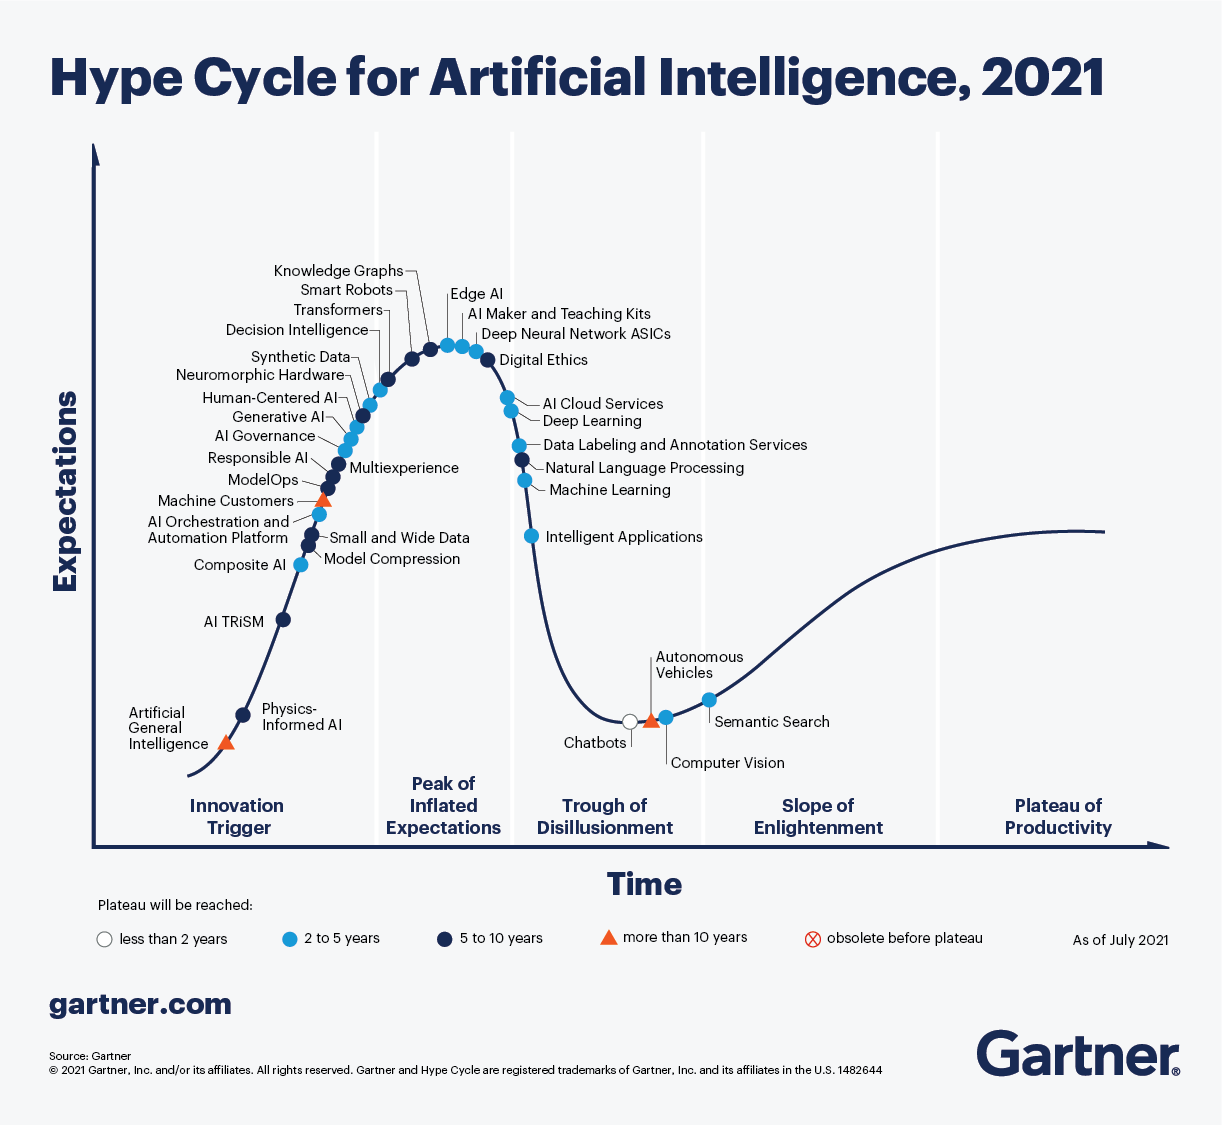
\includegraphics[width=\linewidth]{figures/Ch1/gartner-ai2021.png}
\caption{Hype Cycle for Artificial Intelligence 2021}
\label{f:gartner-ai2021}
\end{figure}

\section{Objectives}
\label{s:Objectives}
The research conducted in this dissertation aims to implement and experiment with different machine learning models to achieve a prediction of time series variables from an industrial field.


\textbf{General Objective:} Develop an intelligent system for industrial variables monitoring and forecasting.

\textbf{Specific Objectives:}

\begin{itemize}
\item Identify and characterize principal variables that carry out a proper forecasting.
\item Develop an intelligent system based on the key variables obtained and different forecasting models.
\item Evaluate each model performance to determine which model is suitable under different testing conditions.
\end{itemize}

\section{Thesis Question}
\label{s:Question}
The principal question addressed in this dissertation is:

¿How accurate can be predicted water quality parameters of an industrial wastewater treatment plant an intelligent system?

\section{Contributions}
\label{s:Contributions}

Our key contributions include:

\begin{enumerate}

  \item Machine Learning algorithms tested in industrial scenario. Specially when a ground-breaking (novel) wastewater treatment is implemented. 
  
  \item Evaluation of different ensemble methods to improve single predictive models for industrial field.

\end{enumerate}

\section{Thesis Outline}
\label{s:Outline}

The remainder of this thesis is organized as follows. 

\begin{description}

  \item[Chapter \ref{c:Background}] presents background information relevant to the field of research. Provide details regarding topics and concepts the reader should know about wastewater treatment and data analysis computational techniques that will be mentioned throughout the thesis.
  
  \item[Chapter \ref{c:Related-Works}] provides a detailed discussion of the major existing contributions to the field and how they relate to each other and the proposed intelligent system.
  
  \item[Chapter \ref{c:Contribution-1}] describe the properties and development process of the 3 machine learning approaches proposed. it details the considerations for all three model designs.
  
  \item[Chapter \ref{c:Contribution-2}] details the properties and development of the ensemble methods implemented to improve the performance of each individual model.
  
  \item[Chapter \ref{c:Experiments}] details testing of the proposed intelligent system and each of its parts. A data-amount sensibility experiment is presented.
  
  \item[Chapter \ref{c:Conclusions}] concludes this thesis. First, it summarizes the work. Then, it highlights interesting aspects of the research and provides a thorough discussion of potential topics and areas, with respect to Machine Learning and Wastewater treatment, that may be interesting for future research activities. 
  
\end{description}




  
  \chapter{Theoretical Framework}\label{c:Background}
  This chapter introduces and reviews general concepts of the wastewater treatment, machine learning techniques for regression.

\section{Wastewater Treatment}
\label{s:First-Background-Topic}

Provide background information that will help potential readers to understand your research. It is up to you to decide the volume and content of this chapter.



\section{Machine Learning}
\label{s:Second-Background-Topic}

\ac{ML} is an area of the \ac{AI} where a computer is programmed to learn form data \cite{Ray2019}. In 1959 Arthur Samuel defined the Machine Learning as \textbf{the field of study that gives the computers the ability to learn without being explicitly programmed}. Almost 40 years later, Tom Mitchell described Machine Learning as follows: \textbf{A computer program is said to learn from experience E with respect to some task T and some performance measure P, if its performance on T, as measured by P, improves with experience E.} \autoref{f:AI} shows the how the \ac{ML} fits in the \ac{AI} world and presents \ac{DL} as part of \ac{ML} which is presented in \autoref{s:Second-Background-Deep-Learning}.

\begin{figure}[h]
\centering
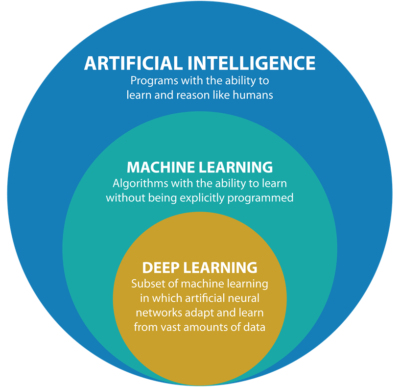
\includegraphics[width=8cm]{figures/Ch2/AI-ML-DL.png}
\caption{AI, ML, and DL \cite{raza_cinquergrana_2018}}
\label{f:AI}
\end{figure}

\begin{figure}[t]
\centering
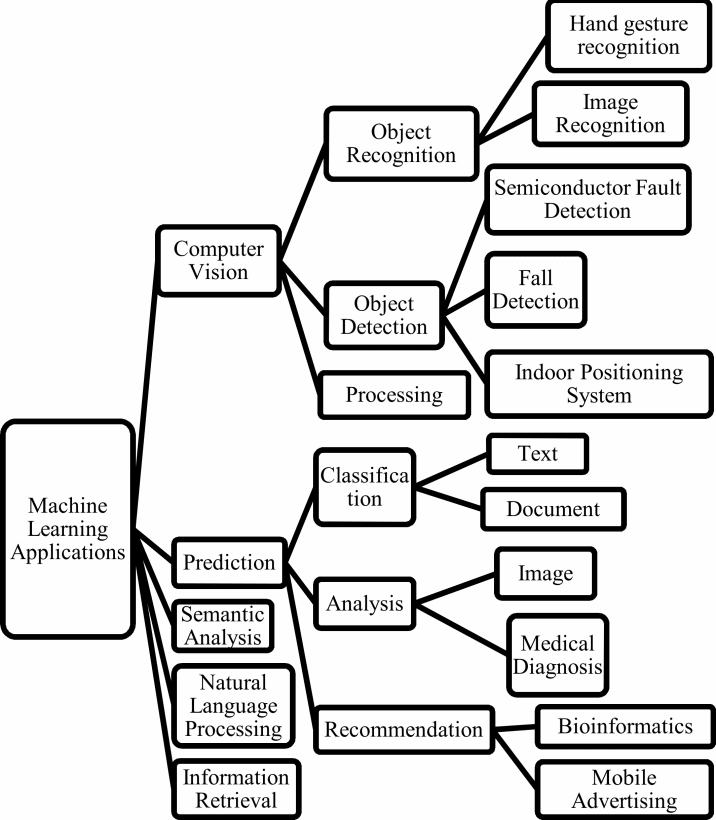
\includegraphics[width=8cm]{figures/Ch2/ML-Applications.png}
\caption{ML Applications \cite{Shinde_2018}}
\label{f:Ml-app}
\end{figure}

Now a days machine Learning is used in a variety of fields such as: robotics, biology, social science, virtual personal assistants, computer games, autonomous driving, pattern recognition, natural language processing, computer vision, product recommendation, market prediction, medical diagnosis, fraud detection, agriculture advisory, Bots, climatology, social media services, among others \cite{Srivastava_2019, Shinde_2018, Ray2019}, \autoref{f:Ml-app} shows some of the \ac{ML} application domains. 

\begin{figure}[h]
\centering
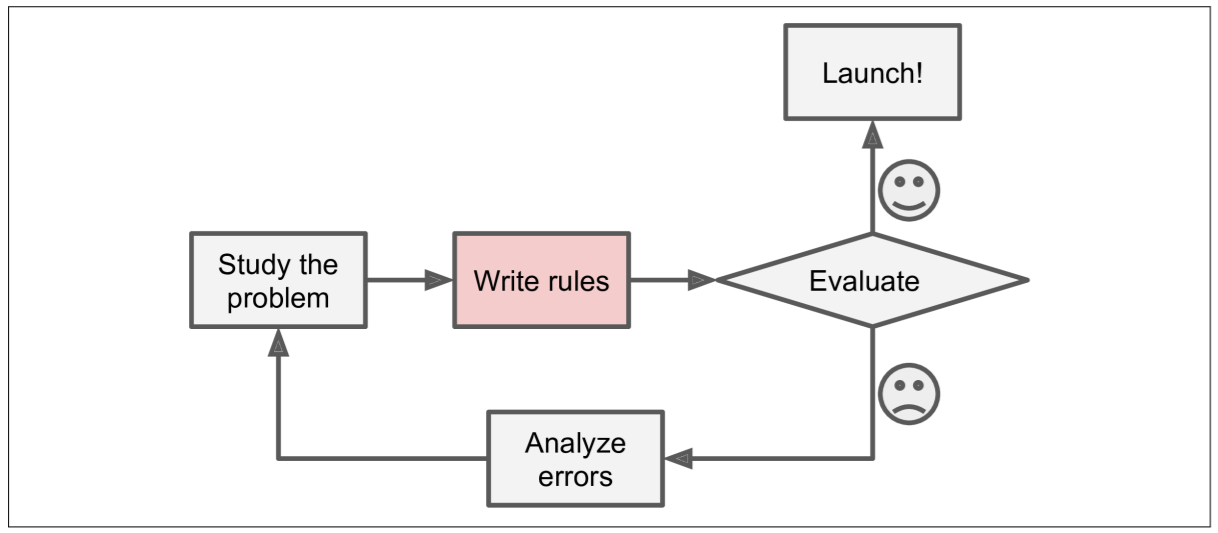
\includegraphics[width=\linewidth]{figures/Ch2/Tradicional-Approach.png}
\caption{Traditional rule based approach \cite{geron2017}}
\label{f:Traditional-approach}
\end{figure}

An important milestone was the transition from rule based programming to programs that learn automatically based on experience by the use of data. \autoref{f:Traditional-approach} shows how the rule based approach works, it starts by studying the problem, identifying some patterns and building a set of rules based on them. Subsequently, the system is evaluated and the rules are adjusted continuously in an iterative process until a good enough performance is achieved \cite{geron2017}. Should be noted that the bigger the problem the more complex the rules and more difficult the pattern identification task becomes. Meanwhile, \ac{ML} programs improve their performance during the training phase, usually presenting shorter programs, more maintainable, and more accurate. Some studies that compare the results of these data analysis methods evidence that the first tends to provide stronger scientifically sounder information, statistical assessment and uncertainty estimations, but the latter tends to bring forward better accuracy in the majority of works \cite{geron2017,Ye2020}. \autoref{f:ML-approach} illustrates the \ac{ML} approach to solve problems.

\begin{figure}[h]
\centering
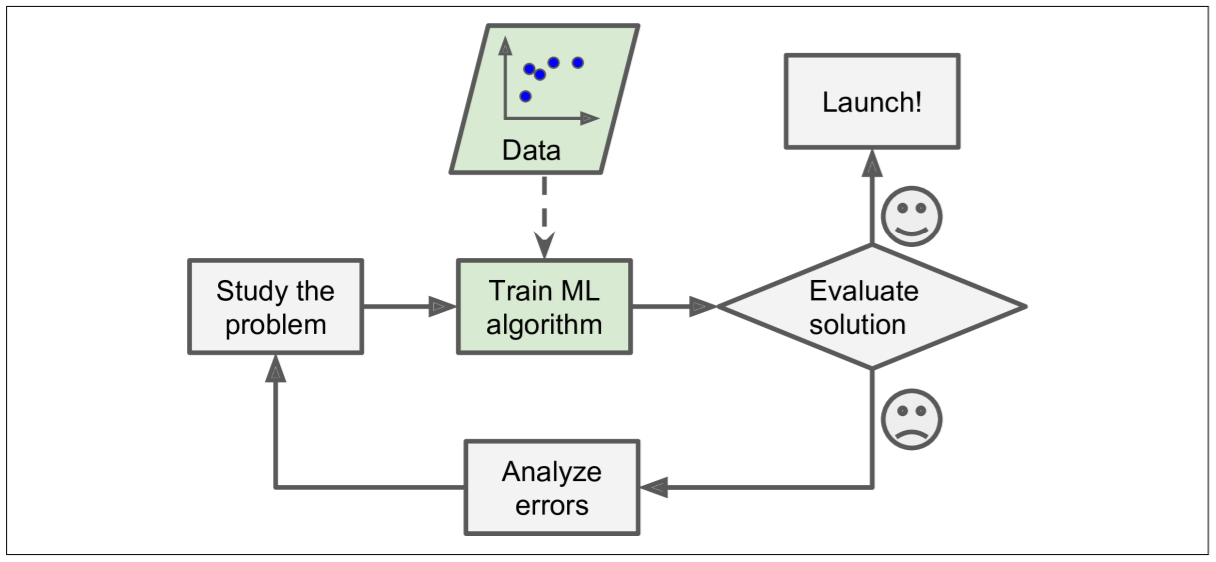
\includegraphics[width=\linewidth]{figures/Ch2/Ml-Approach.png}
\caption{ML approach \cite{geron2017}}
\label{f:ML-approach}
\end{figure}

There are different types of \ac{ML} systems, and they can be classified based on human supervision as supervised learning, unsupervised learning and reinforcement learning. 

\subsection{Supervised Learning}
This category of \ac{ML} algorithms aim to find a function capable of represent the relationship between the input and output variables from a given set of data. It is called supervised since it infers the function from labelled examples during the training stage, which means that for each input sample there is an associated and known output sample assigned by a human supervisor \cite{Batta2020}. 

\begin{figure}[h]
\centering
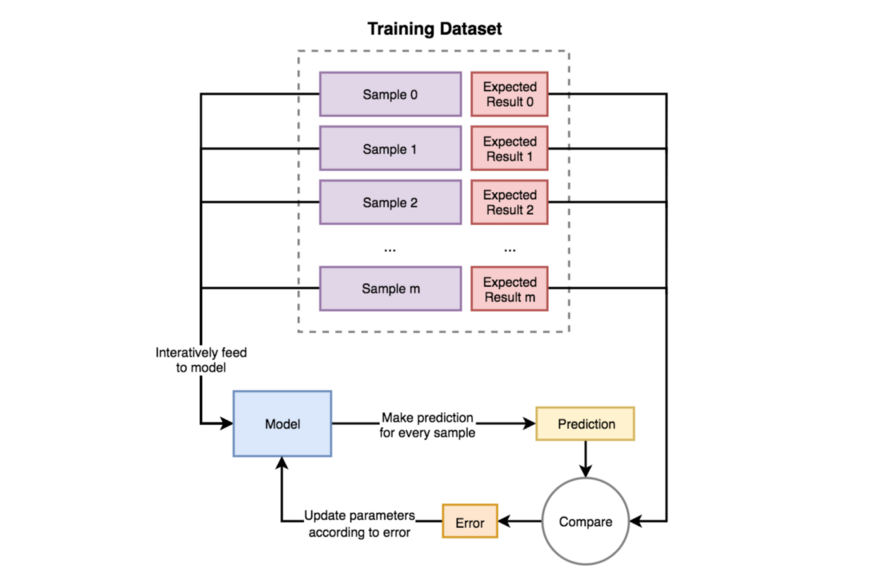
\includegraphics[width=\linewidth]{figures/Ch2/Supervised-Learning.png}
\caption{Supervised Learning}
\label{f:supervised-learning}
\end{figure}

This type of machine learning is used for both regression and classification tasks.

\begin{figure}[h]
\centering
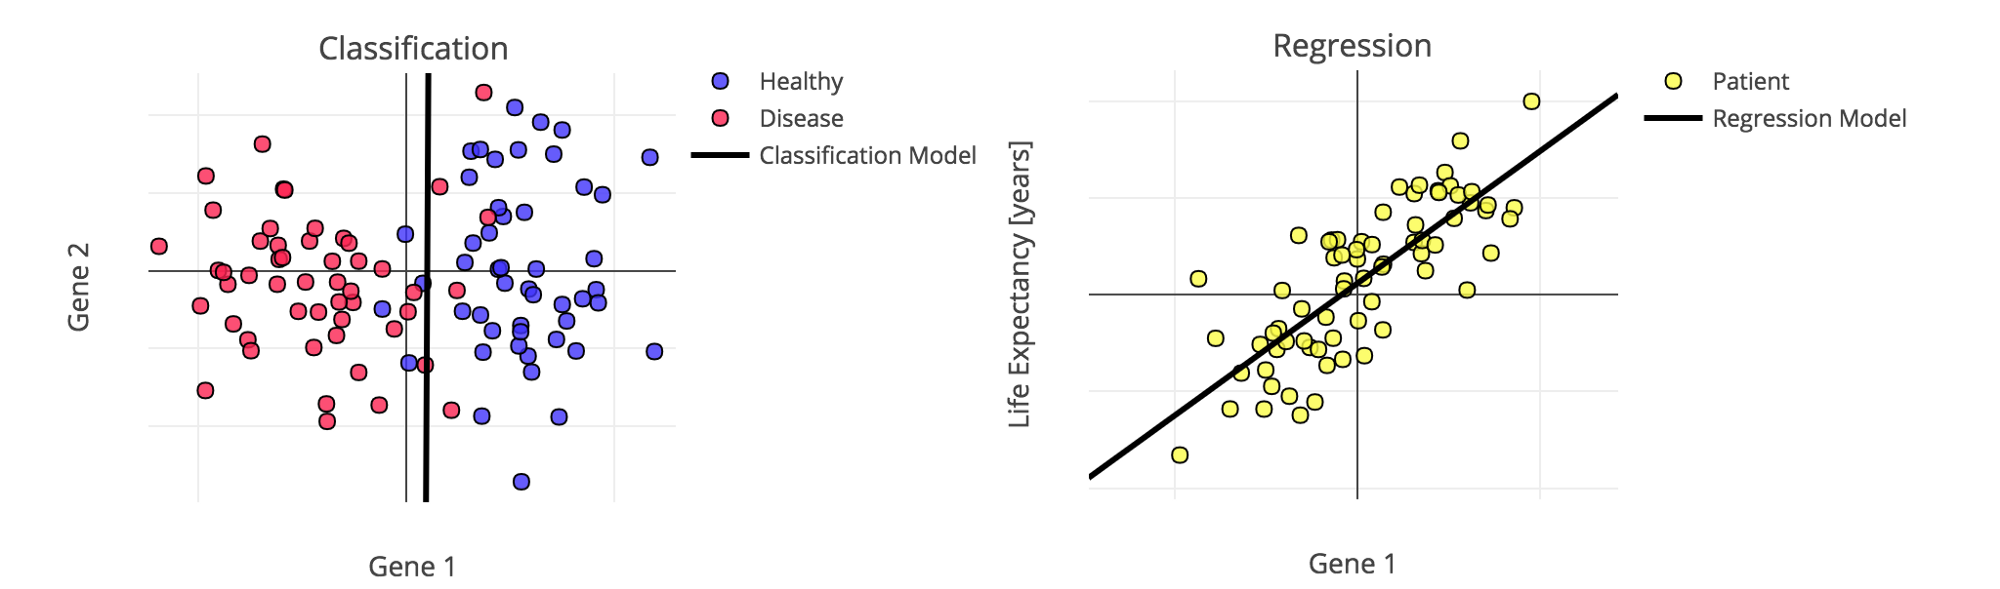
\includegraphics[width=\linewidth]{figures/Ch2/Regression-Classification.png}
\caption{Classification and Regression examples}
\label{f:classification-regression}
\end{figure}

\subsubsection{Linear Regression}
\subsubsection{Decision Tree}
\subsubsection{Support Vector Machines}

\subsection{Unsupervised Learning}
\subsubsection{PCA}
\subsubsection{Clustering}


\section{Deep Learning}
\label{s:Second-Background-Deep-Learning}

\begin{figure}[h]
\centering
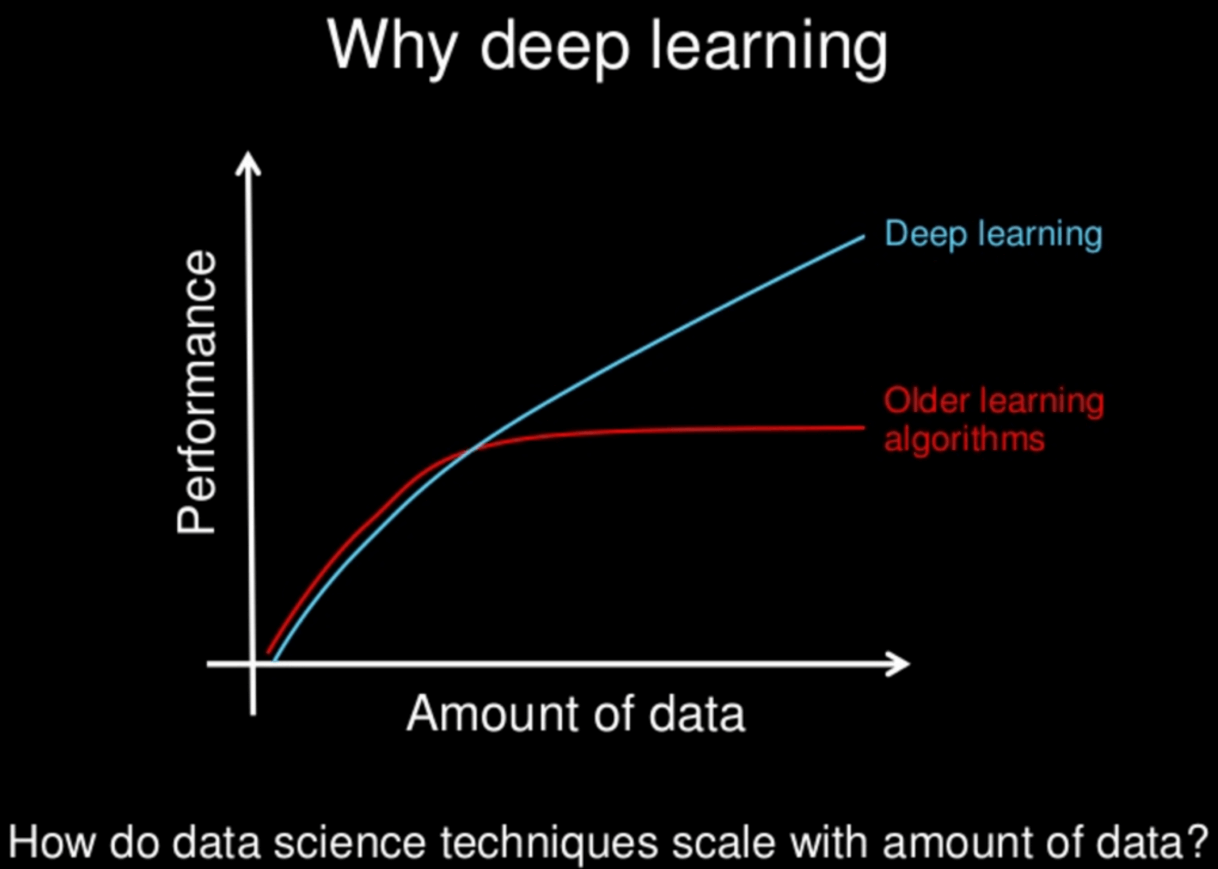
\includegraphics[width=8cm]{figures/Ch2/MlvsDL-data-amount.png}
\caption{ML vs DL}
\label{f:ML-vs-DL}
\end{figure}

\section{Evaluation Metrics}
\label{sec:section_Example}
\subsection{Mean Absolute Percentage Error}
\subsubsection{Determination Coefficient}

\section{Summary}
\label{s:Background-Summary}

The final section of each chapter should summarize the chapter. In comparison to the chapter.


  
  \chapter{Related Works}\label{c:Related-Works}
  This chapter presents an overview of the main works focused on the topics addressed in this dissertation.

\section{Related Works Description}
\label{s:RelatedWorks-Description}

The state-of-the-art presents different computational techniques for data analysis. Lots of works found in the \ac{WWT} field use a combination of them to achieve their goal and improve the operation of the \acs{WWTP}s. Most works aim to accomplish fault detection, control, soft-sensing, variable prediction, or process understanding, among others. Special attention will be given to the prediction task since it is the main focus of this investigation.
%either physical modelling, can have different purposes,

\ac{WWTP}s are systems that exhibit a complex dynamic and require high performance to accomplish the standards imposed by the environmental regulatory authorities \cite{Corominas2018}. Considering the complex process nature, which presents a nonlinear behaviour and involves the interaction of physical, chemical, and biological components, it becomes crucial to estimate and predict key process variables. These variable predictions enhance the control, process monitoring and simulation that increase the efficiency of the treatment and the quality of the effluent \cite{Aalami2019,Arismendy2020,Liu2020}. Artificial intelligence methods are commonly used for solving the estimation and prediction challenges in nonlinear engineering science problems \cite{Lotfi2019}. Literature introduces a wide landscape of strategies and techniques to achieve the prediction task. 
\autoref{f:Techniques-Distribution} \cite{Corominas2018} shows the distribution of computational techniques used in the field of wastewater treatment for fault detection, prediction, soft-sensing, process understanding, control and optimization, among others, it is made based on the number of papers published and cited in recent years. 

\begin{figure}[t]
\centering
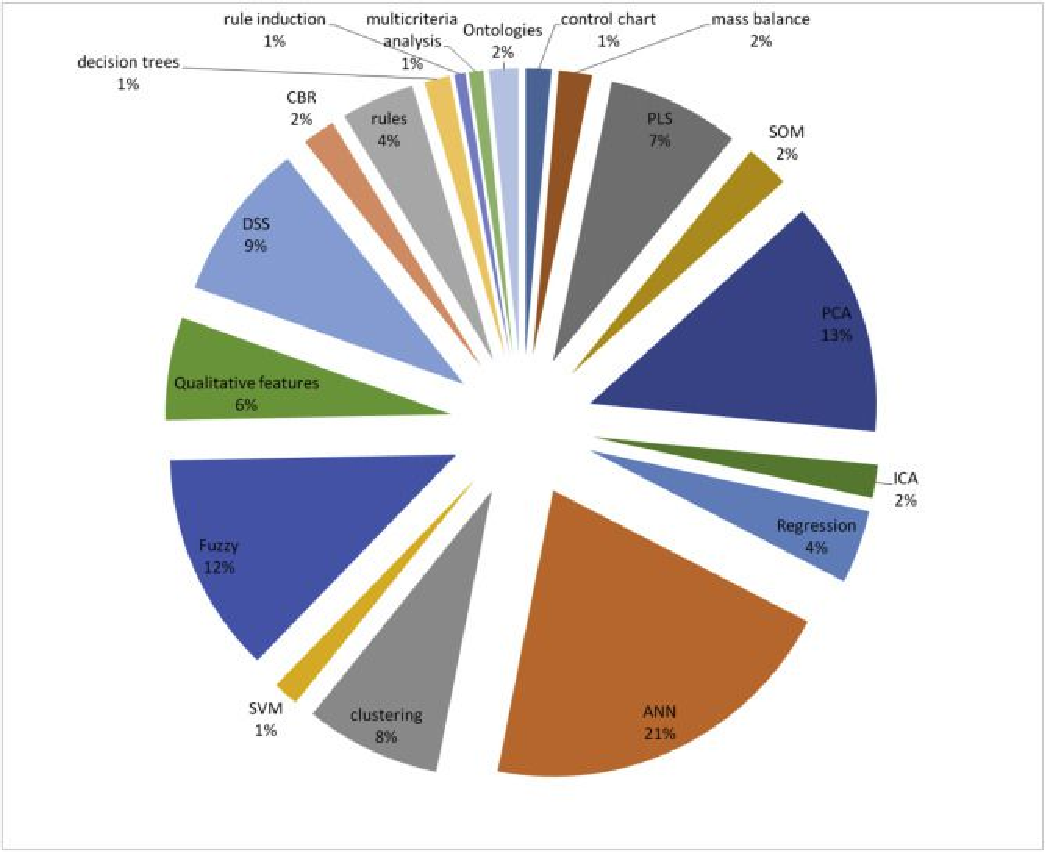
\includegraphics[width=15cm]{figures/Ch3/Computational-techniques-in-wwtp.pdf}
\caption{Techniques distribution \cite{Corominas2018}.}
\label{f:Techniques-Distribution}
\end{figure}

Research carried out by \cite{Corominas2018} shows that most of the papers published use \ac{ANN}, \ac{PCA} and \ac{FL} which are present in 46\% of the papers studied. Regarding the prediction tasks, which is the focus of this work, \ac{MLR} models, \ac{FL}, \ac{PLS}, \ac{ANN} and \ac{SVM} are the main methods used, where the last two stand out on nonlinear supervised learning. Other techniques involved in prediction are \ac{PCA}, Self-organizing Maps \ac{SOM}, clustering, and Qualitative features commonly used for dimensionality reduction, information extraction, problem understanding, and variable selection.

One of the early approximations to intelligent monitoring and the predicting system was presented in \cite{Sanguesa2000}, and \cite{Haggege2005}, where Bayesian networks and neuro-fuzzy logic were implemented to fulfil limitations of rule-based systems. Further works started to focus their attention on variable prediction using various methods and a combination of them, taking the major advantages offered by each one. Reference \cite{Qin2012} used iterative predictor weighting–partial least squares boosted by weighted predictions of a collection of regression models used as an ensemble prediction to estimate some water quality parameters. It was tested in the field, and its results showed a high correlation of the prediction. 

Several recent studies used fuzzy logic or neuro-fuzzy systems, such as \cite{Nourani2018,Nadiri2018,Han2018}, and some deep learning approaches, as in \cite{Guo2015,Alsina2018,Dairi2019}, which have provided high performance in prediction tasks. Studies like \cite{Bagheri2015} used a hybrid artificial neural network–genetic algorithm approach to optimize the \ac{ANN} estimation of the sludge bulking present in the sedimentation stage, which directly affects the effluent discharge water quality. Reference \cite{Dellana2009} made a performance comparison between the \ac{ARIMA} and time-delay neural network \ac{TDNN} with such times-series variables as \ac{BOD} and \ac{TSS} and achieved more accurate predictions for real-world wastewater data with \ac{TDNN}.

\section{Variable Prediction}
\label{s:RelatedWorks-variablePrediction}

\cite{Zhou2019} proposes a set of decision-tree regression models to predict daily wastewater influent in two \ac{WWTP}s located in Ontario. Results for training and testing exhibit a \begin{math}R^2\end{math} of 0.97 and 0.72 for one facility and the second one 0.96 and 0.58, respectively. \cite{Lu2020} evaluates the performance of two decision-tree-based ensemble learners and enhances their performance with a data denoising technique called \ac{CEEMDAN} to predict Temperature, Dissolved Oxygen, pH, Specific Conductance, and fluorescent dissolved organic matter. The enhanced Extreme Gradient Boosting and \ac{RF} show the best results among other techniques used in the experiments, obtaining \ac{MAPE}s from 0.27\% to 14.94\% in the best cases, depending on the variable selected to predict.

Study \cite{Alsulaili2021} implements a \ac{FFNN} to predict the effluent \ac{BOD}, \ac{COD} and \ac{TSS} in Kabd \ac{WWTP}, Kuwait. The authors train the model with 1032 samples and take as input different influent parameters. This work presents a \begin{math}R^2\end{math} score of 0.75, 0.61 and 0.63, respectively. Also, \cite{Abba2017} determines the efficiency of \ac{ANN} in predicting effluent \ac{COD} of Nicosia \ac{WWTP}, Chipre. Six different \ac{ANN} models are trained where diverse model structures, input variables and epochs of training are considered. The best results obtained present a \begin{math}R^2\end{math} of 0.70 which is an improvement compared with the baseline they established using \ac{MLR} and obtained \begin{math}R^2\end{math} of 0.34.

Work \cite{Niu2020} proposes a hybrid predictive model that uses \ac{DBN}, a  structure specialized in regression tasks. A \ac{GA} optimizes the hyperparameters of the network achieving a \ac{MAPE} of 4.34\% and \begin{math}R^2\end{math} of 0.6 for the effluent \ac{COD} prediction.

Reference \cite{Zhao2021} compares the impact of the optimization algorithm used during the training of a \ac{FFNN} implemented with the aim of predicting effluent \ac{TN}. The baseline model uses backpropagation optimization algorithm and achieves a \begin{math}R^2\end{math} value of 0.85 and 0.26 for training (104 data points) and testing dataset (20 data points), respectively. The implementation of \ac{L-M}, \ac{BR}, and Scaled Conjugate Gradient optimization algorithms shows an improvement in the overfitting of the baseline model, obtaining \begin{math}R^2\end{math} of 0.88, 0.84, and 0.84 during training and 0.87, 0.78, and 0.86 over the whole set respectively.

Another example \cite{Manu2017} compares the performance of  \ac{SVM}s and \ac{ANFIS} in the prediction of discharge \ac{TN} concentration for the Kavoor \ac{WWTP} located at Mangalore. \ac{ANFIS} are fuzzy logic systems where the structure is replaced by a neural network. Experiments show that \ac{SVM}s overcome the results obtained by the \ac{ANFIS}, achieving a \begin{math}R^2\end{math} of 0.82 versus 0.62 with Trapezoid Membership Functions and 0.72 with Gaussian Membership Functions. 

Work \cite{Guo2015} aims to predict one-day interval \ac{TN} concentration of effluent stream from Yong-yeon \ac{WWTP} in Ulsan, Korea. Measurements of some parameters from different points of the treatment serve as inputs for two \ac{ML} models: \ac{ANN} and \ac{SVM}. Results show a \begin{math}R^2\end{math} for training and validation of 0.55 and 0.47 for the \ac{ANN} and 1.00 and 0.46 for the \ac{SVM} approach. Both models use 200 and 90 samples for training and validation process, respectively.

Recurrent neural networks are also used in wastewater data-driven modelling. \cite{Yaqub2020} uses \ac{LSTM} Neural Networks to predict removal efficiency of NH4-N, \ac{TN}, and \ac{TP} from a \ac{WWTP} at Okcheon, Republic of Korea. A year of data with hourly frequency measurements constitutes the dataset used for this work. A set of 5000 data points build the sequences of 10 previous observations used to train the  \ac{LSTM} model. The testing step shows the \ac{MSE} values of 0.0047, 0.015, and 0.018, respectively, by using 1876 new data points. Study \cite{Kang2020} proposes a \ac{LSTM} and compares the results with \ac{SVM}, \ac{GRU} Neural Network, and standard  \ac{Bi-LSTM}. Experiments show that \ac{Bi-LSTM} performs at least as well as other models and obtain better results in some scenarios.

A \ac{GRNN} is implemented in \cite{Heddam2016}, a network architecture made of four layers: the input layer, the pattern layer, the summation layer, and the output one. This architecture offers high performance in non-linear regression analysis, the reason why it is used to estimate the effluent \ac{BOD} based on other effluent parameters. Results are compared with a \ac{MLR} showing that the \ac{GRNN} performs better for the \ac{BOD} estimation, achieving \begin{math}R^2\end{math} of 0.75 and 0.80 for training and testing, where 553 and 138 samples are respectively used. 

\cite{Baki2019} test the predictive capabilities of diverse regression models used to estimate the \ac{BOD} in the Antalya Hurma \ac{WWTP}. The study implements four different methods; classical regression analysis, Multivariate Adaptive Regression Splines, Artificial Bee Colony, and teaching learning-based optimization. \cite{Baki2019} uses 186 samples corresponding to 80\% of the available data to train all four proposed techniques, which yield \begin{math}R^2\end{math} values of 0.74, 0.79, 0.78, and 0.74 over the test dataset.

\cite{Guo2020} innovates in the use of \ac{CNN} together with \ac{RNN}s. The system proposed uses a convolution layer, a pooling layer, and a fully connected layer as feature extractor, followed by an \ac{LSTM} to achieve the \ac{COD} and Ammonia Nitrogen prediction in the outlet of a sewage treatment plant located in Nan'an District, Chongqing, China.

Work \cite{Nourani2018} compares the performance of \ac{FFNN}, \ac{ANFIS}, \ac{SVR}, and \ac{MLR} models to predict \ac{COD}, \ac{BOD}, and \ac{TN} at the Nicosia \ac{WWTP} effluent stream. An averaging unit combines the output of the four models improving the final prediction up to 24\%. Three different ensemble techniques are implemented, all of them present R2 higher than 0.8 in validation. Another example of ensemble learner \cite{Nourani2021} utilizes \ac{FFNN}, \ac{SVR}, \ac{ANFIS}, and \ac{ARIMA} to predict \ac{COD} and \ac{BOD} effluent in Tabriz \ac{WWTP}. Additional to the ensemble jittered data is used to enhance the model learning capabilities. Results show that both ensemble techniques and jittered data improved the system predictive performance where the ensemble jittering model exhibits \begin{math}R^2\end{math} of 0.85/0.86 (\ac{COD}/\ac{BOD}) in comparison with \begin{math}R^2\end{math} of 0.82/0.81 with the standard ensemble model.

\section{Intelligent Control}
\label{s:RelatedWorks-Control}

Less common but also present in the state-of-the-art, some hybrid models combine mechanistic, heuristic and data-driven models. As an example, \cite{Hvala2020} improves the predictive performance of a mechanistic model based on the ASM2d model (\ac{ASM} version 2d) using a Gaussian process technique increasing the \begin{math}R^2\end{math} value from 0.61 to 0.8 for effluent \ac{TN} and from 0.54 to 0.65 for effluent \ac{TP}.

In \cite{Pang2019}, a \ac{QL} algorithm with an activated sludge model (\ac{ASM}2d-guided) reward setting was proposed. The integrated \ac{ASM}2d-QL algorithms equipped with a self-learning mechanism were derived for optimizing the control strategies \ac{HRT} and \ac{IRR}) of the \ac{WWTP} system. In \cite{Li2013}, a Bayesian network-based approach was proposed for real-time prediction of a wastewater treatment system based on \ac{MSBR}. Based on the framework of the modified sequencing batch reactor prediction analysis, a Bayesian network model was constructed to analyze an \ac{MSBR} using training data and information provided by domain experts.

Work \cite{Haggege2005} is a synthesis of a new neuro-fuzzy controller with an online learning procedure and a simple algebraic formulation, making it easy to interpret by a human being to control a bioreactor without requiring any analytical representation. The authors in \cite{Nadiri2018} focused on the Tabriz \ac{WWTP}, proposing an ensemble of \ac{FL}, \ac{CFL}  and supervised \ac{CFL} to predict water quality parameters. In \cite{Nourani2018}, three nonlinear models (\ac{FFNN}, \ac{ANFIS} and \ac{SVM}s) and a classical \ac{MLR} were applied to predict the performance of the Nicosia wastewater treatment plant in terms of \ac{BOD}, \ac{COD} and \ac{TN}. 

In work \cite{Bagheri2015}, multilayer perceptron \ac{ANN}–genetic algorithm and radial basis function \ac{ANN}–genetic algorithm models were successfully implemented for \ac{SVI} prediction, taking into account that when sludge bulking appears, it causes poor settleability of sludge that results in poor effluent quality, loss of active biomass and increased costs and poses several environmental hazards. \ac{BOD}, \ac{COD}, nitrate, ammonia, \ac{TN}, \ac{TP}, \ac{TSS}, total dissolved solids, \ac{MLVSS}, \ac{MLSS}, \ac{SVI}, \ac{DO}, pH and temperature were measured and used for the estimation. The study \cite{Raduly2007} performed a simulation of plant behaviour over a wide range of influent disturbances. An \ac{ANN} was trained on the available \ac{WWTP}, comparing \ac{ANN} and a mechanistic \ac{WWTP} model’s performances.

The study \cite{Liukkonen2013} proposed the Kohonen \ac{SOM}, a helpful tool for illustrating the prevailing states of a process and their evolution, monitoring the alteration of wastewater quality and alerting in case of unusual behaviour, such as increasing concentrations of harmful discharge components. The method provided an advanced and efficient way of monitoring and visualizing many measurements conducted in wastewater treatment. Article \cite{Jimenez2015} emphasized the high potential of some promising techniques, such as spectral analysis, and discussed issues that could appear soon concerning control of anaerobic digestion processes. The authors in work \cite{Reis2017} provided a critical outlook of the evolution of \ac{IPM} since its introduction almost 100 years ago. Several evolution trends that have been structuring \ac{IPM} developments over this extended period were briefly referred to, with more focus on data-driven approaches.

Reference \cite{Ye2020} is a review of developments in artificial intelligence technologies for environmental pollution controls, including prediction of removal efficiency, evaluation of fuzzy logic to the control of the \ac{WWTP} aerobic stage and \ac{AI}-aided soft sensors for estimation of hard-to-measure variables. 

\section{Fault Detection}
\label{s:RelatedWorks-faultDetection}

There is a research branch whose aim is opportune fault detection in very stringent processes, especially when it is part of the critical operational path where any unexpected event leads to stagnation. Depending on the type of fault detection, the prediction of the problem can be focused on:

\begin{itemize}
 \item	The system’s ability to operate under some given circumstances.
 \item	The time range in which equipment needs no maintenance and logistic support \cite{Alsina2018}.
\end{itemize}

Regarding system operability, analyzing some patterns in \ac{WWTP} data allows detecting faults and their potential causes even before they occur. The data visualization can show patterns that are products of a possible anomaly, known as abnormal patterns. These are classified as isolated, sustained, transient and drift \cite{Newhart2019}. Each one provides a hint about a future fault. Thus, it is possible to get fault information by looking at data behaviour. Reference \cite{Dairi2019} implemented data-driven unsupervised anomaly detection approaches based on deep learning methods and clustering algorithms. The aim was to monitor and detect anomaly conditions in \ac{WWTP} operations. The results showed its ability to spot the vast majority of abnormal events reported by the operator \cite{Dairi2019}. 

 Reference \cite{Alsina2018} showed how machine learning models obtained better prediction results concerning traditional methods when increasing the size of the time-to-failure datasets. It implements four diverse machine learning approaches: \ac{ANN}, \ac{SVM}, \ac{RF} and soft computing methods. Work \cite{Dairi2019} presented a data-driven anomaly detection approach based on deep learning methods and clustering algorithms to monitor influent conditions of \ac{WWTP}, which affect treatment unit states, ongoing process mechanisms and product qualities. These techniques were \ac{RNN} and the function to delineate complex distributions from \ac{RBM}, with various classifiers.
 
 On the other hand, basic reliability analysis focuses on predicting the period in which equipment needs no support. This technique allows for finding a probability function R(t) to forecast the performance time of a component without failing until a given period t \cite{Alsina2018}. The work of \cite{Alsina2016} used an \ac{ANN} to find the best cumulative failure distribution of mechanical components, which had a performance to fit a set of failure data and estimate its parameters, especially under poor data conditions. As a result, the networks with a momentum equal to 0.75 produced the best approximation 83.46\% of the time \cite{Alsina2016}.

\section{Soft-Sensing}
\label{s:Related-Works-SoftSensing}

Work \cite{Zounemat-Kermani2019} is a survey of the feasibility of utilizing soft computing models in predicting emission factors based on five input parameters, namely, the total dissolved sulfides, biochemical oxygen demand (\ac{BOD}\textsubscript{5}), temperature, flow rate and pH. Multivariate \ac{NARX} neural networks were developed and applied to predict weekly H2S in four \ac{WWTP}s. The paper \cite{Yu2019} described an optimized extreme learning machine based on an improved cuckoo search algorithm for the design of the soft \ac{BOD} measurement model.

The study \cite{Hernandez-del-Olmo2019} performed different machine learning techniques to model a soft sensor to predict weather conditions such as \ac{SVM}s, \ac{KNN}, \ac{DT}, \ac{RF}s and Gaussian \ac{NB}. An advanced control system can fit the parameters for better performance with accurate weather prediction.

For paper \cite{Han2018}, a data-driven intelligent monitoring system was implemented (using the soft sensor technique and data distribution service). A fuzzy neural network was applied for designing the soft sensor model.

\cite{Shen2018} compares the performance of four models; a multi-layer perceptron Neural Network trained with \ac{L-M} algorithm, a backpropagation trained Neural Network, a \ac{RBNN}, and a \ac{GRNN}. All four models are trained with 410 samples representing the 75\% of the whole data, and the results show that \ac{RBNN} outperform the others obtaining a \ac{MAPE} of 13.7\%/14.4\% and \begin{math}R^2\end{math} of 0.92/0.91 for training and validation, respectively.

Other research introduces the use of \ac{FL} especially combined with another computational technique to enhance its performance. \cite{Huang2015} uses a \ac{NFS} combined with a \ac{GA} to estimate real-time nutrient concentrations in a biological stage of a wastewater treatment process. The GA-NFS soft-sensor estimates nitrogen and phosphorus concentration, and \ac{COD} obtaining \ac{MAPE}s of 16.18\%, 24.56\% and 7.8\% respectively. They encourage the addition of the GA component comparing this \ac{GA}-\ac{NFS} with a simple \ac{NFS}, which obtained \ac{MAPE}s of 31.86\%, 26.19\% and 22.79\% for each variable, demonstrating the impact of the optimization.

\section{Data Tools}
\label{s:Related-Works-Data-Tools}

Nowadays, since the world creates new data every second, it has had to look for technologies to treat this data properly. In the market, some of them are Apache Hadoop and SciDB (open source) and others owned by super companies like Google, IBM, Amazon and Microsoft (frameworks) \cite{Siddiqui2015}. Each framework is specialized to do a particular task. A review \cite{Valentin-Vargas2012} synthesized these frameworks as shown in \autoref{t:data_tools_table} (adapted from \cite{Valentin-Vargas2012}). Besides, the main languages for analytics, data mining and data science are Python, R, and SAS. Each language has weaknesses and strengths. However, according to a Burtch Works poll (2019), computer scientists and engineers preferred using Python, as shown in \autoref{f:soft-preferences}

%\begin{longtable}{@{}l *{2}{rr}}
\begin{longtable}[h]{@{}l *{2}{rr}}
\caption[Data analytic Tools]{Data analytic Tools}
\label{t:data_tools_table}
\\
%   
\toprule%


 {\bfseries Area} & {\bfseries Amazon} & {\bfseries Microsoft} & {\bfseries Google}
\\

\cmidrule[0.4pt](r{0.125em}){1-1}%
\cmidrule[0.4pt](lr{0.125em}){2-4}%
%\cmidrule[0.4pt](lr{0.125em}){4-5}%
%\cmidrule[0.4pt](lr{0.125em}){5-6}%


  \endfirsthead

\endhead

    Big data storage & S3 & Azure & Google Cloud services  \\ 
    Big data analytics & Elastic MapReduce & Hadoop on Azure & BigQuery  \\
     &  (Hadoop) &  &   \\ 
    Relational database  & MySQL or Oracle & SQL Azure & Cloud SQL  \\ 
    NoSQL database & DynamoDB & Table storage & App Engine Datastore  \\ 
    MapReduce & Elastic MapReduce & Hadoop on Azure & App Engine  \\ 
     &  (Hadoop) &  &  \\ 
    Streaming  & Nothing prepackaged & StreamInsight & Search API  \\ 
    processing &  &  &   \\ 
    Machine learning & Hadoop + Mahout & Hadoop + Mahout & Prediction API  \\ 
    Data sources & Public datasets & Windows Azure  & A few sample datasets  \\ 
     &   & marketplace &   \\ 
    Availability & Public production & Some services  & Some services \\
     &  & in private beta & in private beta  \\


\bottomrule

\end{longtable}

\begin{figure}[h]
\centering
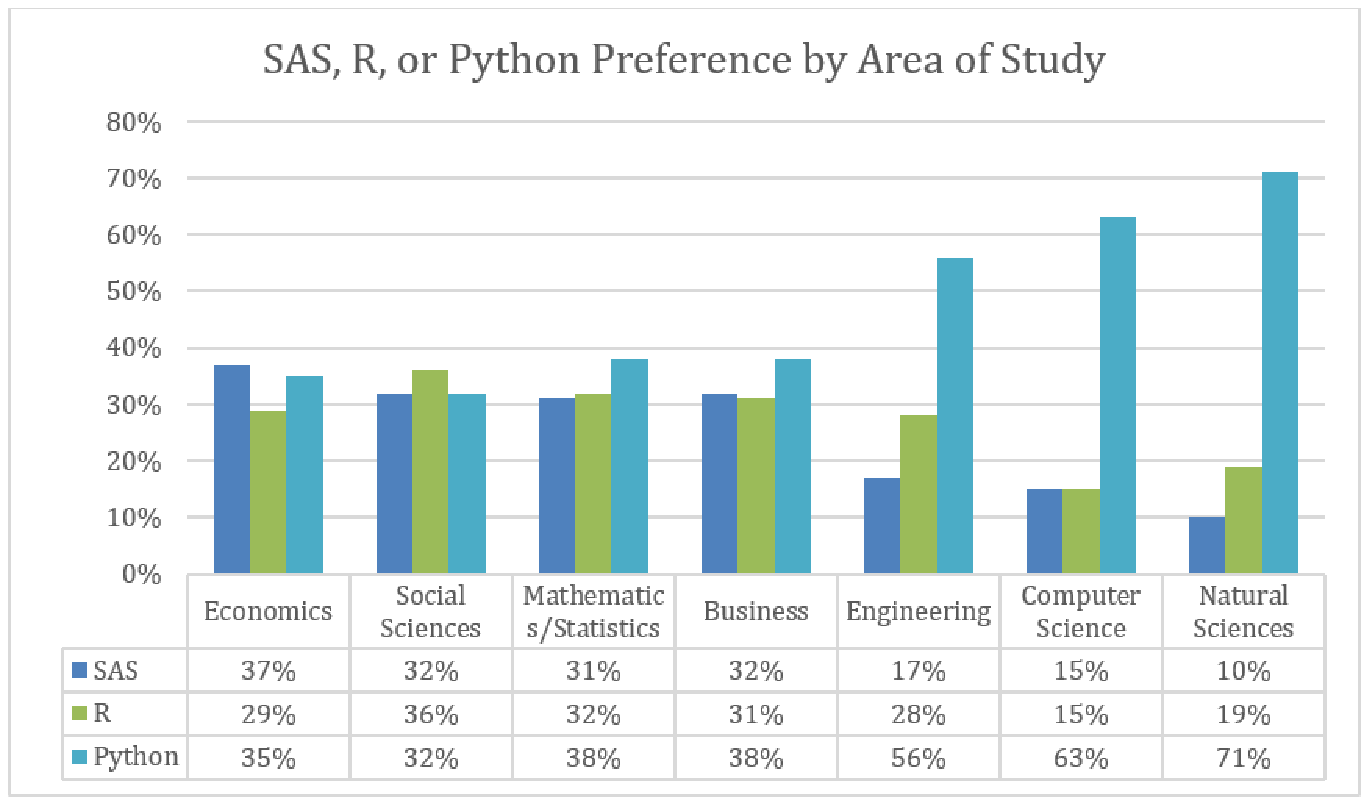
\includegraphics[width=\linewidth]{figures/Ch3/BigDataTools.pdf}
\caption{SAS, R or Python preferences \cite{Siddiqui2015}}
\label{f:soft-preferences}
\end{figure}

\begin{figure}[h]
\centering
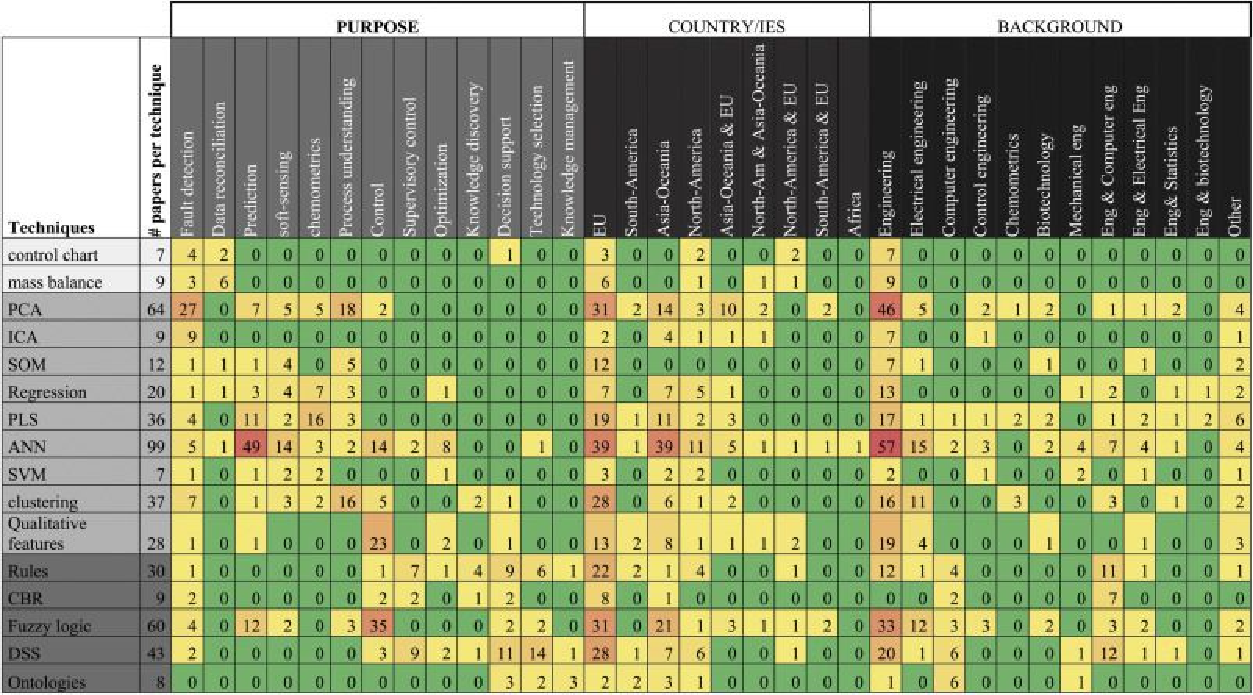
\includegraphics[width=0.9\linewidth]{figures/Ch3/PaperTable.pdf}
\caption{Techniques in WWT  \cite{Corominas2018}.}
\label{f:Papers Table}
\end{figure}

\begin{figure}[h]
\centering
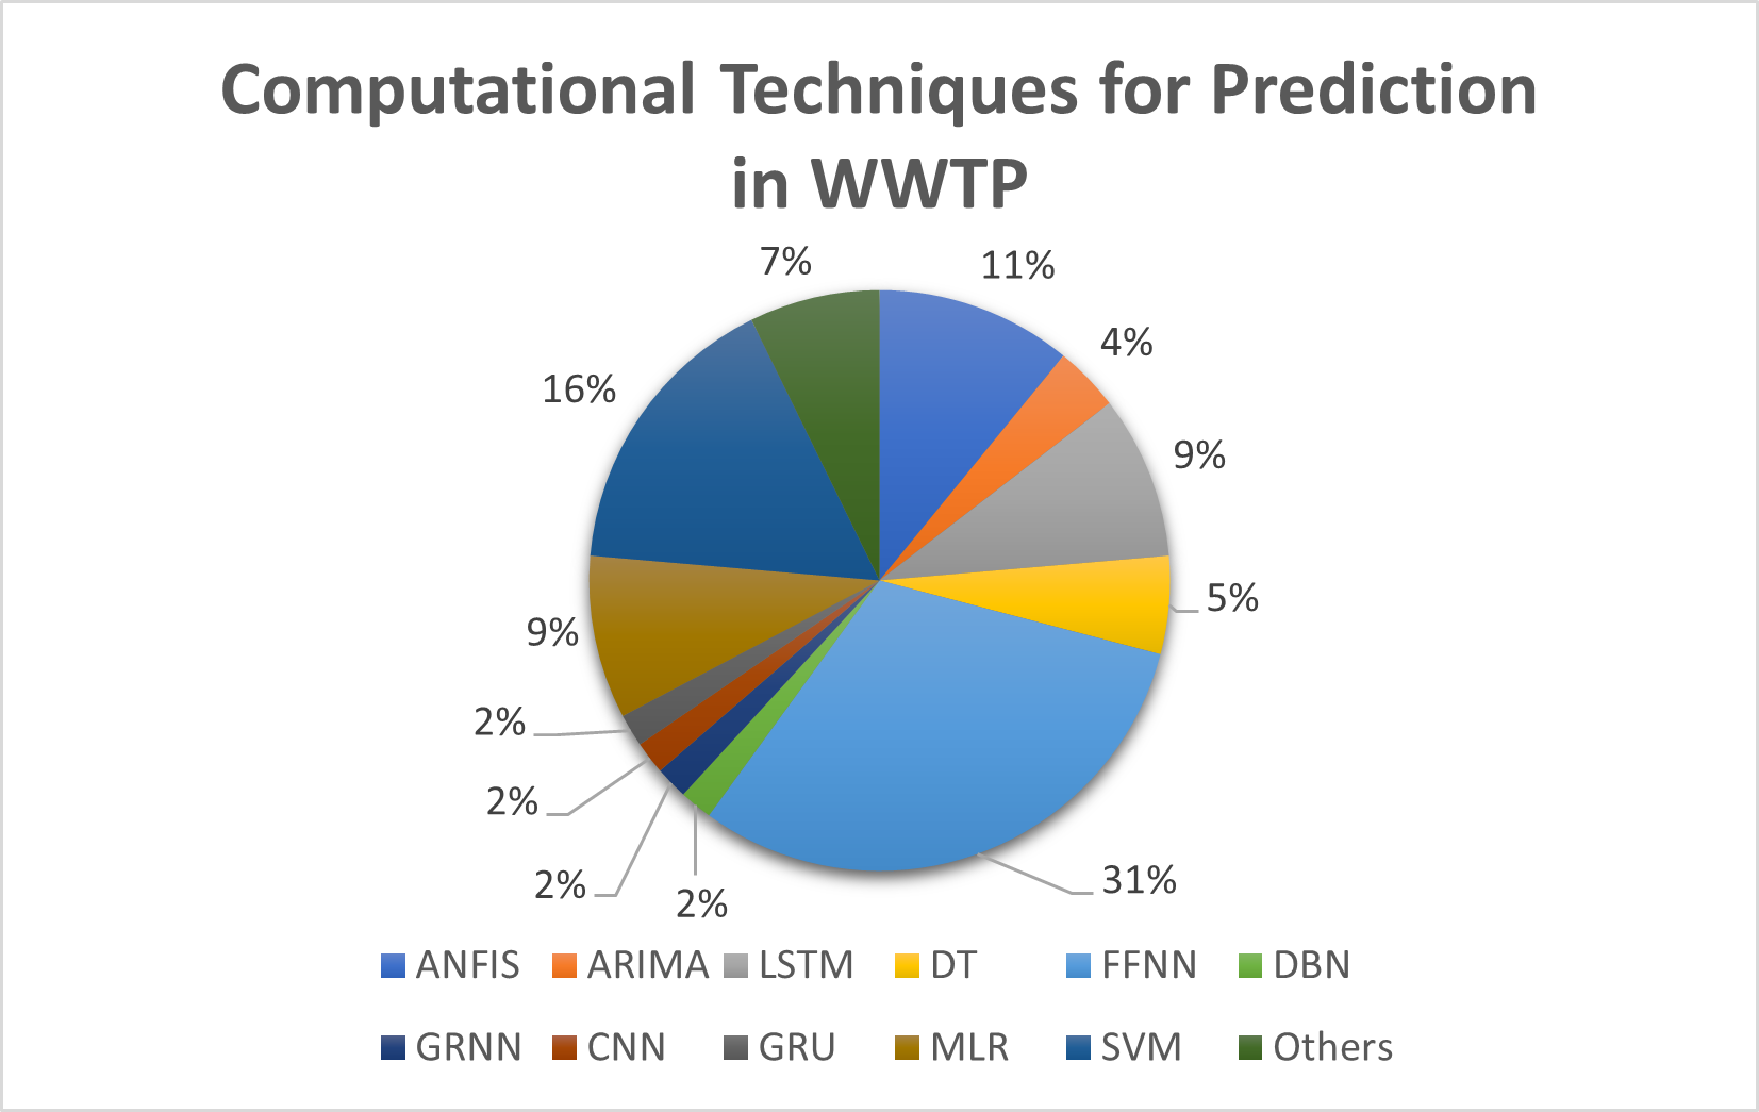
\includegraphics[width=0.8\linewidth]{figures/Ch3/Prediction_model_dist.pdf}
\caption{Techniques used for Prediction in WWT field}
\label{f:techniques-prediction}
\end{figure}

\autoref{f:Papers Table} presented by \cite{Corominas2018} shows the number of papers per technique used in \ac{WWT}, categorized based on purposes, countries and the authors' background. The search was done in SCOPUS, and the results include papers until 2015, papers published before 2010 and with less than five citations were not included. \autoref{f:techniques-prediction} summarizes the \ac{ML} techniques distribution used for prediction and presented in \autoref{s:RelatedWorks-variablePrediction}. \ac{FFNN}, \ac{ANFIS}, \ac{SVM} are place in the top three being the most used ones.
%\section{Summary}
%\label{s:Related-Works-Summary}
  
  \chapter{Major Contribution 1}\label{c:Contribution-1}
  \ac{COD} is one of the most important variables in the process of a biological treatment since experts can make decisions based on the measurements of this variable. The objective of biological wastewater treatment is to perform a removal of the pollutants present in water. Thus, this treatment is used overall because it is compelling and more efficient than numerous mechanical or compound procedures. In the bioreactor at this stage, a variety of microorganisms are used to break down organic matter in the water. However, the microorganisms are susceptible to change, depending on several the bioreactor conditions. Likewise, it results relevant monitoring the concentration of biomass available in the bioreactor which indicates the state of the microorganisms population.

This study proposes to predict one-day time-window \ac{COD}\textsubscript{D}, \ac{COD}\textsubscript{EQ}, and \ac{MLVSS}, essential parameters in decision-making, knowing how contaminated the water will be at the effluent stream (discharge point), the organic matter concentration at the input of the bioreactor, and how the microorganism population in charge of the biological stage is going to behave. 

\begin{figure}[h]
\centering
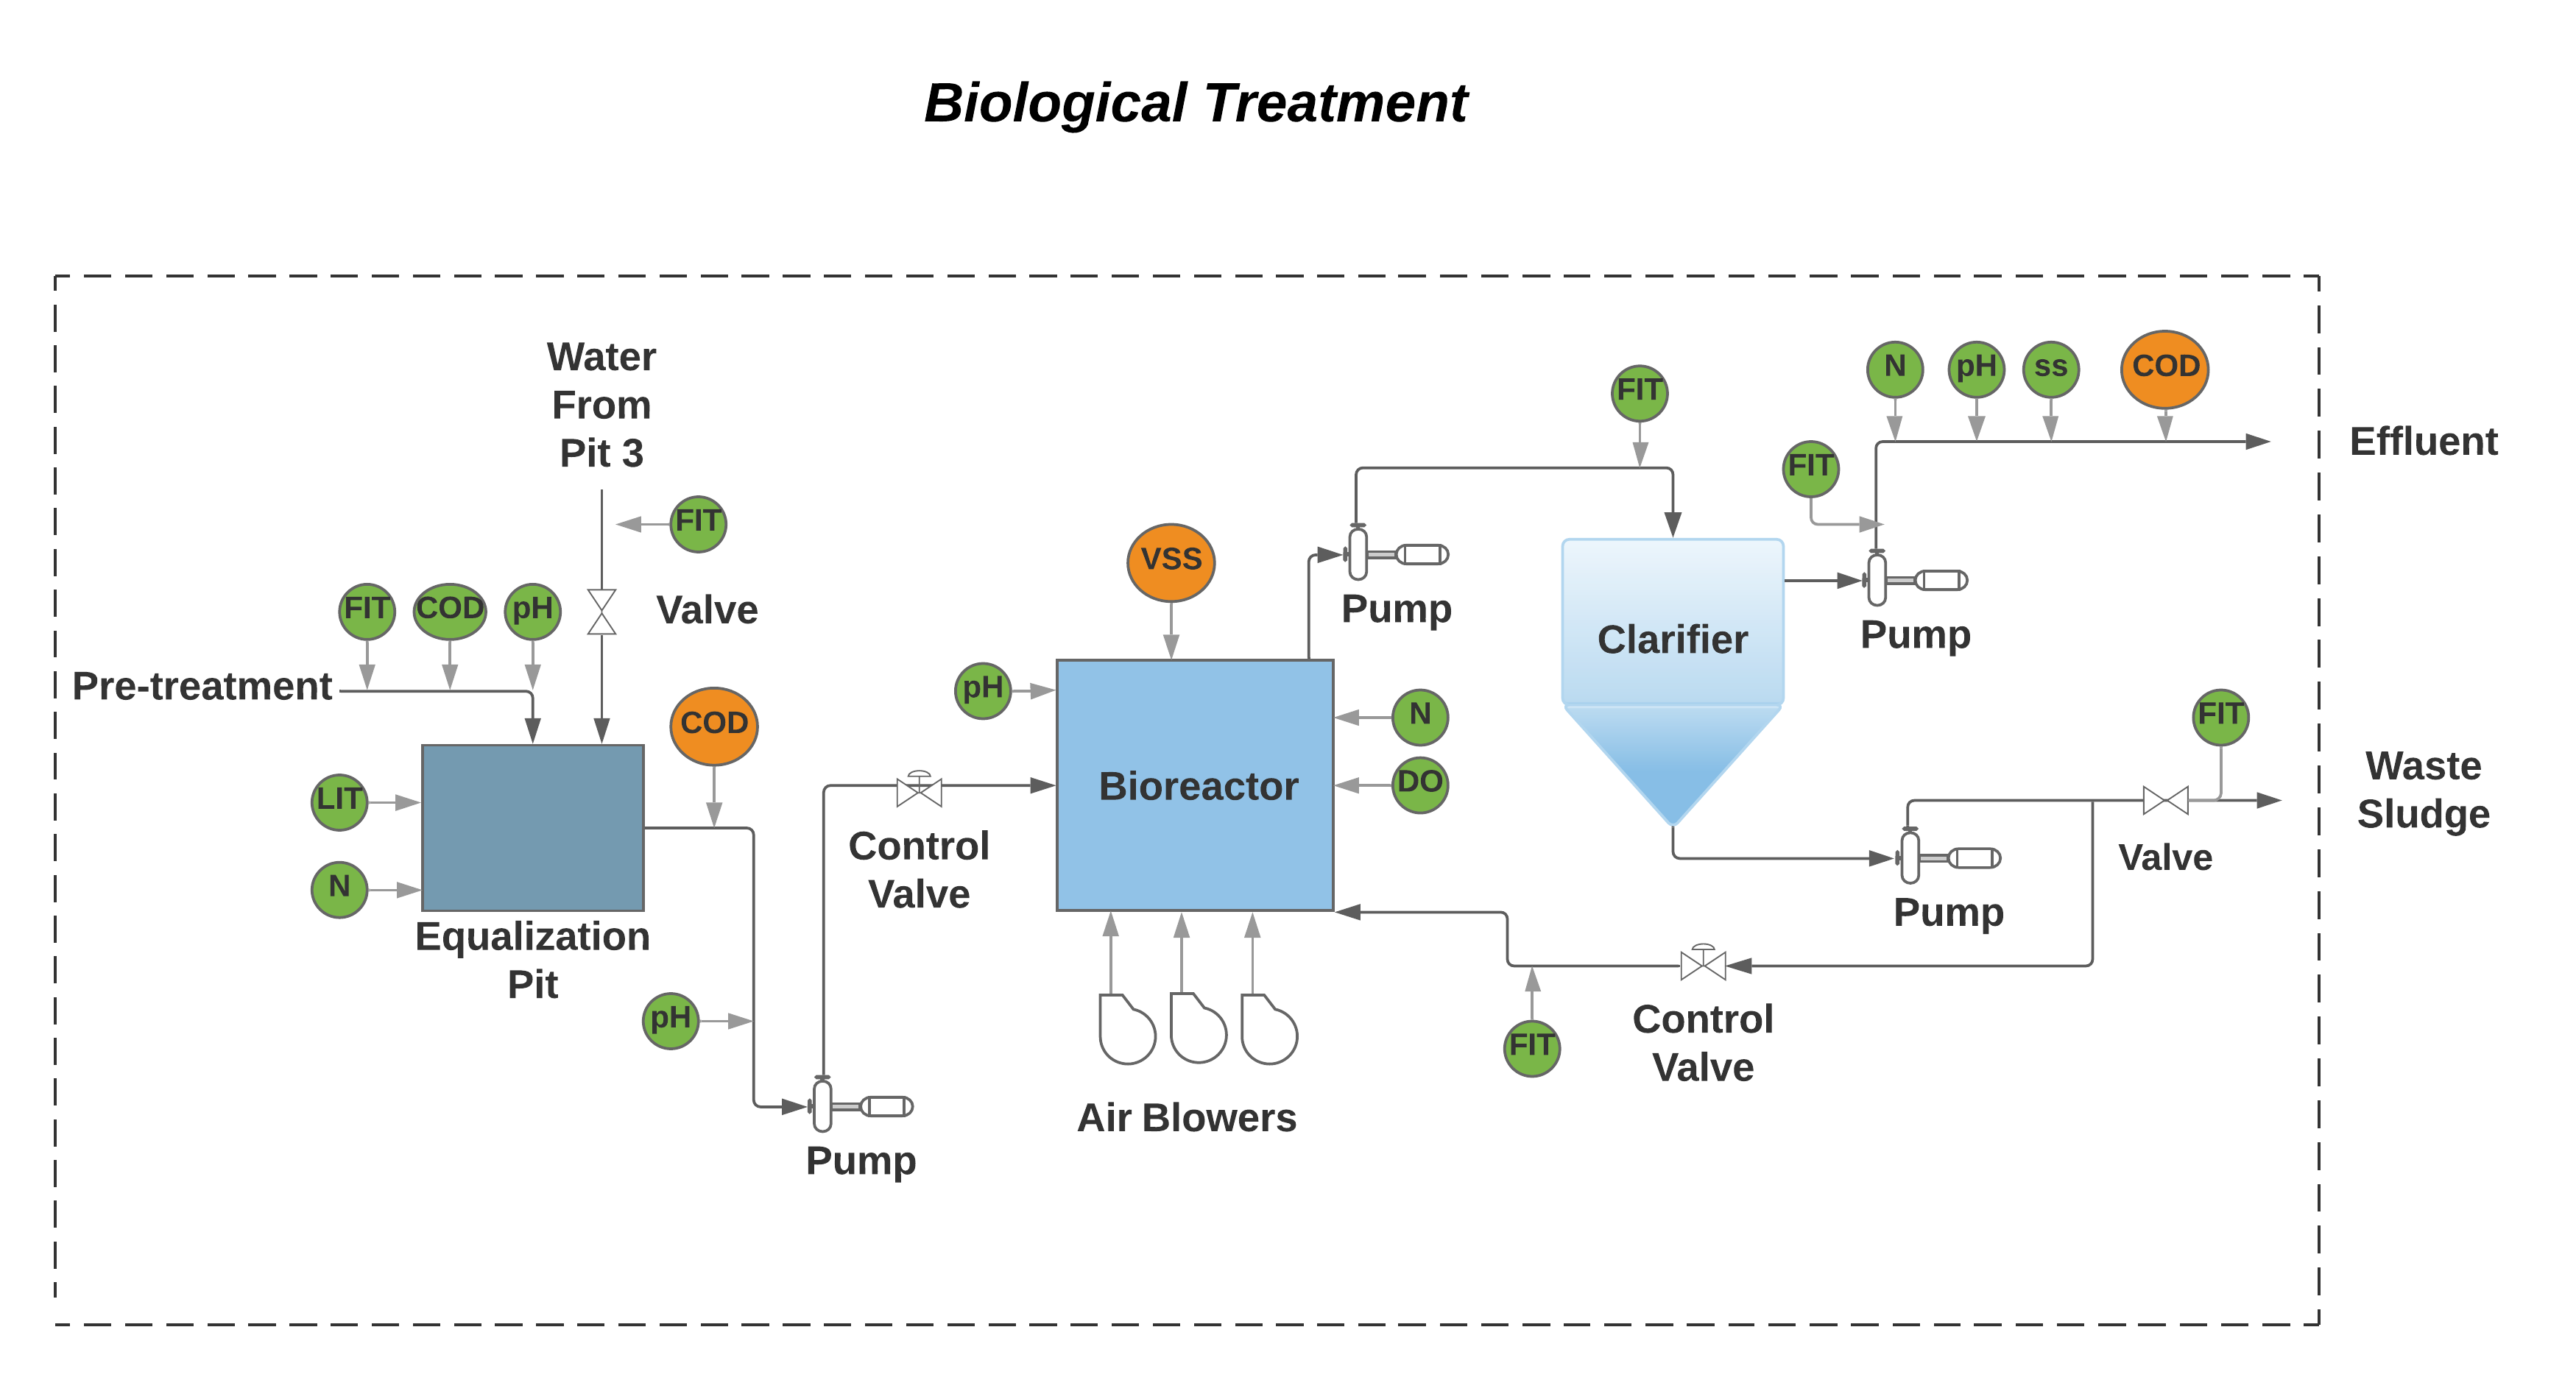
\includegraphics[width=\linewidth]{figures/Ch4/Biological-treatment-stage.png}
\caption{Biological Treatment Stage}
\label{f:Biological-treatment}
\end{figure}

\autoref{f:Biological-treatment} illustrates the composition of the biological treatment stage which is the case of study in this research. The stage has three main components and each one plays an important role in the organic load removal, an equalization pit, a bioreactor, and a clarifier. Green circles represent measured variables of interest and potential input variables for the system. Orange circles are the target variables of this work, which are also available.

This work uses python programming language to implement the intelligent system, supported by several libraries such as Numpy, Pandas, Tensor Flow, Sci-kit Learn, Matplotlib, among others. A GitHub repository contains the files corresponding to code, models, and some of the results presented in this document \footnote{\url{https://github.com/carloscp3009/Machine-Learning-Approaches-for-Industrial-data-forecasting}}. 

The study utilizes 343 data samples from a wastewater treatment facility located in Nantong, China. Measurements correspond to most of the year 2018 and present a daily frequency, which experts consider accurate to capture the process dynamics. The measured variables of the process available for this work are:

\begin{itemize}
 \item	Flow
 \item	COD of influent water
 \item	Suspended solids in influent water (SS)
 \item	Mixed liquor suspended solids (MLSS)
 \item	Mixed liquor volatile suspended solids (MLVSS)
 \item	Nitrogen (N)
 \item	pH
 \item	Mixed liquor dissolved oxygen (DO)
 \item	Food to microorganism (F/M)
\end{itemize}

The following nomenclature determines the unit process or component within the biological stage that the variable is measured.

\begin{itemize}
 \item	EQ = Equalizer
 \item	BIO = Bioreactor
 \item	BT\textsubscript{N}= Bioreactor Pit N
 \item	BT\textsubscript{C}= Bioreactor Pit C
 \item	Clari = Clarifier
 \item	OxT = Oxidation Tank
 \item	D = Discharge Pit
\end{itemize}

%\begin{longtable}{@{}l *{2}{rr}}
\begin{longtable}[h!]{@{}l *{2}{rr}}
\caption[Portrait Table, short caption]{Variables Correlation}
\label{t:correlation_table}
\\
%   
\toprule%


 {\bfseries Variable} & {\bfseries COD\textsubscript{D} } & {\bfseries COD\textsubscript{EQ}} & {\bfseries MLVSS}
\\

\cmidrule[0.4pt](r{0.125em}){1-1}%
\cmidrule[0.4pt](lr{0.125em}){2-4}%
%\cmidrule[0.4pt](lr{0.125em}){4-5}%
%\cmidrule[0.4pt](lr{0.125em}){5-6}%


  \endfirsthead

\endhead

        Flow\_to\_EQ & 0.14 & -0.14 & -0.025  \\ 
        BT\_C\_MLSS & 0.11 & -0.43 & 0.88  \\ 
        BT\_C\_MLVSS & 0.10 & -0.45 & 0.9  \\ 
        BT\_N\_MLSS & 0.10 & -0.44 & 0.88  \\ 
        BT\_N\_MLVSS & 0.10 & -0.44 & 0.88  \\ 
        D\_SS & 0.3 & 0.59 & -0.46  \\ 
        EQ\_N & 0.25 & 0.74 & -0.54  \\ 
        BT\_C\_N & 0.25 & 0.49 & -0.54  \\ 
        BT\_N\_N & 0.11 & 0.26 & -0.47  \\ 
        D\_N & 0.11 & 0.23 & -0.46  \\ 
        OxT\_pH & -0.12 & -0.33 & 0.27  \\ 
        EQ\_pH & -0.069 & 0.18 & -0.17  \\ 
        BT\_N\_pH & 0.057 & -0.045 & 0.083  \\ 
        D\_pH & 0.059 & -0.13 & 0.078  \\ 
        BT\_N\_DO & -0.1 & -0.37 & 0.14  \\ 
        BT\_C\_DO & -0.28 & -0.33 & 0.34  \\ 
        Clari\_DO & -0.17 & -0.43 & 0.27  \\ 
        ST\_COD & 0.22 & 0.63 & -0.44  \\ 
        D\_COD\_ON & 0.72 & 0.22 & 0.11  \\


\bottomrule

\end{longtable}
\autoref{t:correlation_table} presents the Person correlation of the three target variables this study cover. The correlation coefficient allows to select the exogenous variables used as inputs for the system. This enhances the model learning capability by reducing the noise of not correlated variables and decreasing the number of trainable parameters which implies a model complexity reduction. 

After variable selection, the dataset is split into training (0.8), validation (0.1) and test (0.1) sets. The first 80\% of the dataset serves as examples for the model to learn, the following 10\% allows to validate the model performance for early stopping, and hyper-parameters tuning, and the last 10\% is used to evaluate the performance of the model using new data, this way obtaining a certainty of its behaviour in production mode. 

It is important to note that a computational technique must be selected. As mentioned before in related works in \autoref{t:state-of-art}, about 64.71\% of the work of authors used an algorithm from the ANN group to develop forecast models. It has been verified that neural networks have suitable results in the area since the water treatment process is characterized by being nonlinear, so if they are used properly, they can represent the dynamics of this process very well. 

Once a technique is selected, the training of the model begins. An error measure is necessary to support the performance of the model. Therefore, defined as shown in \autoref{eq:MAPE} is used as the evaluation metric.

\begin{figure}[h]
\centering
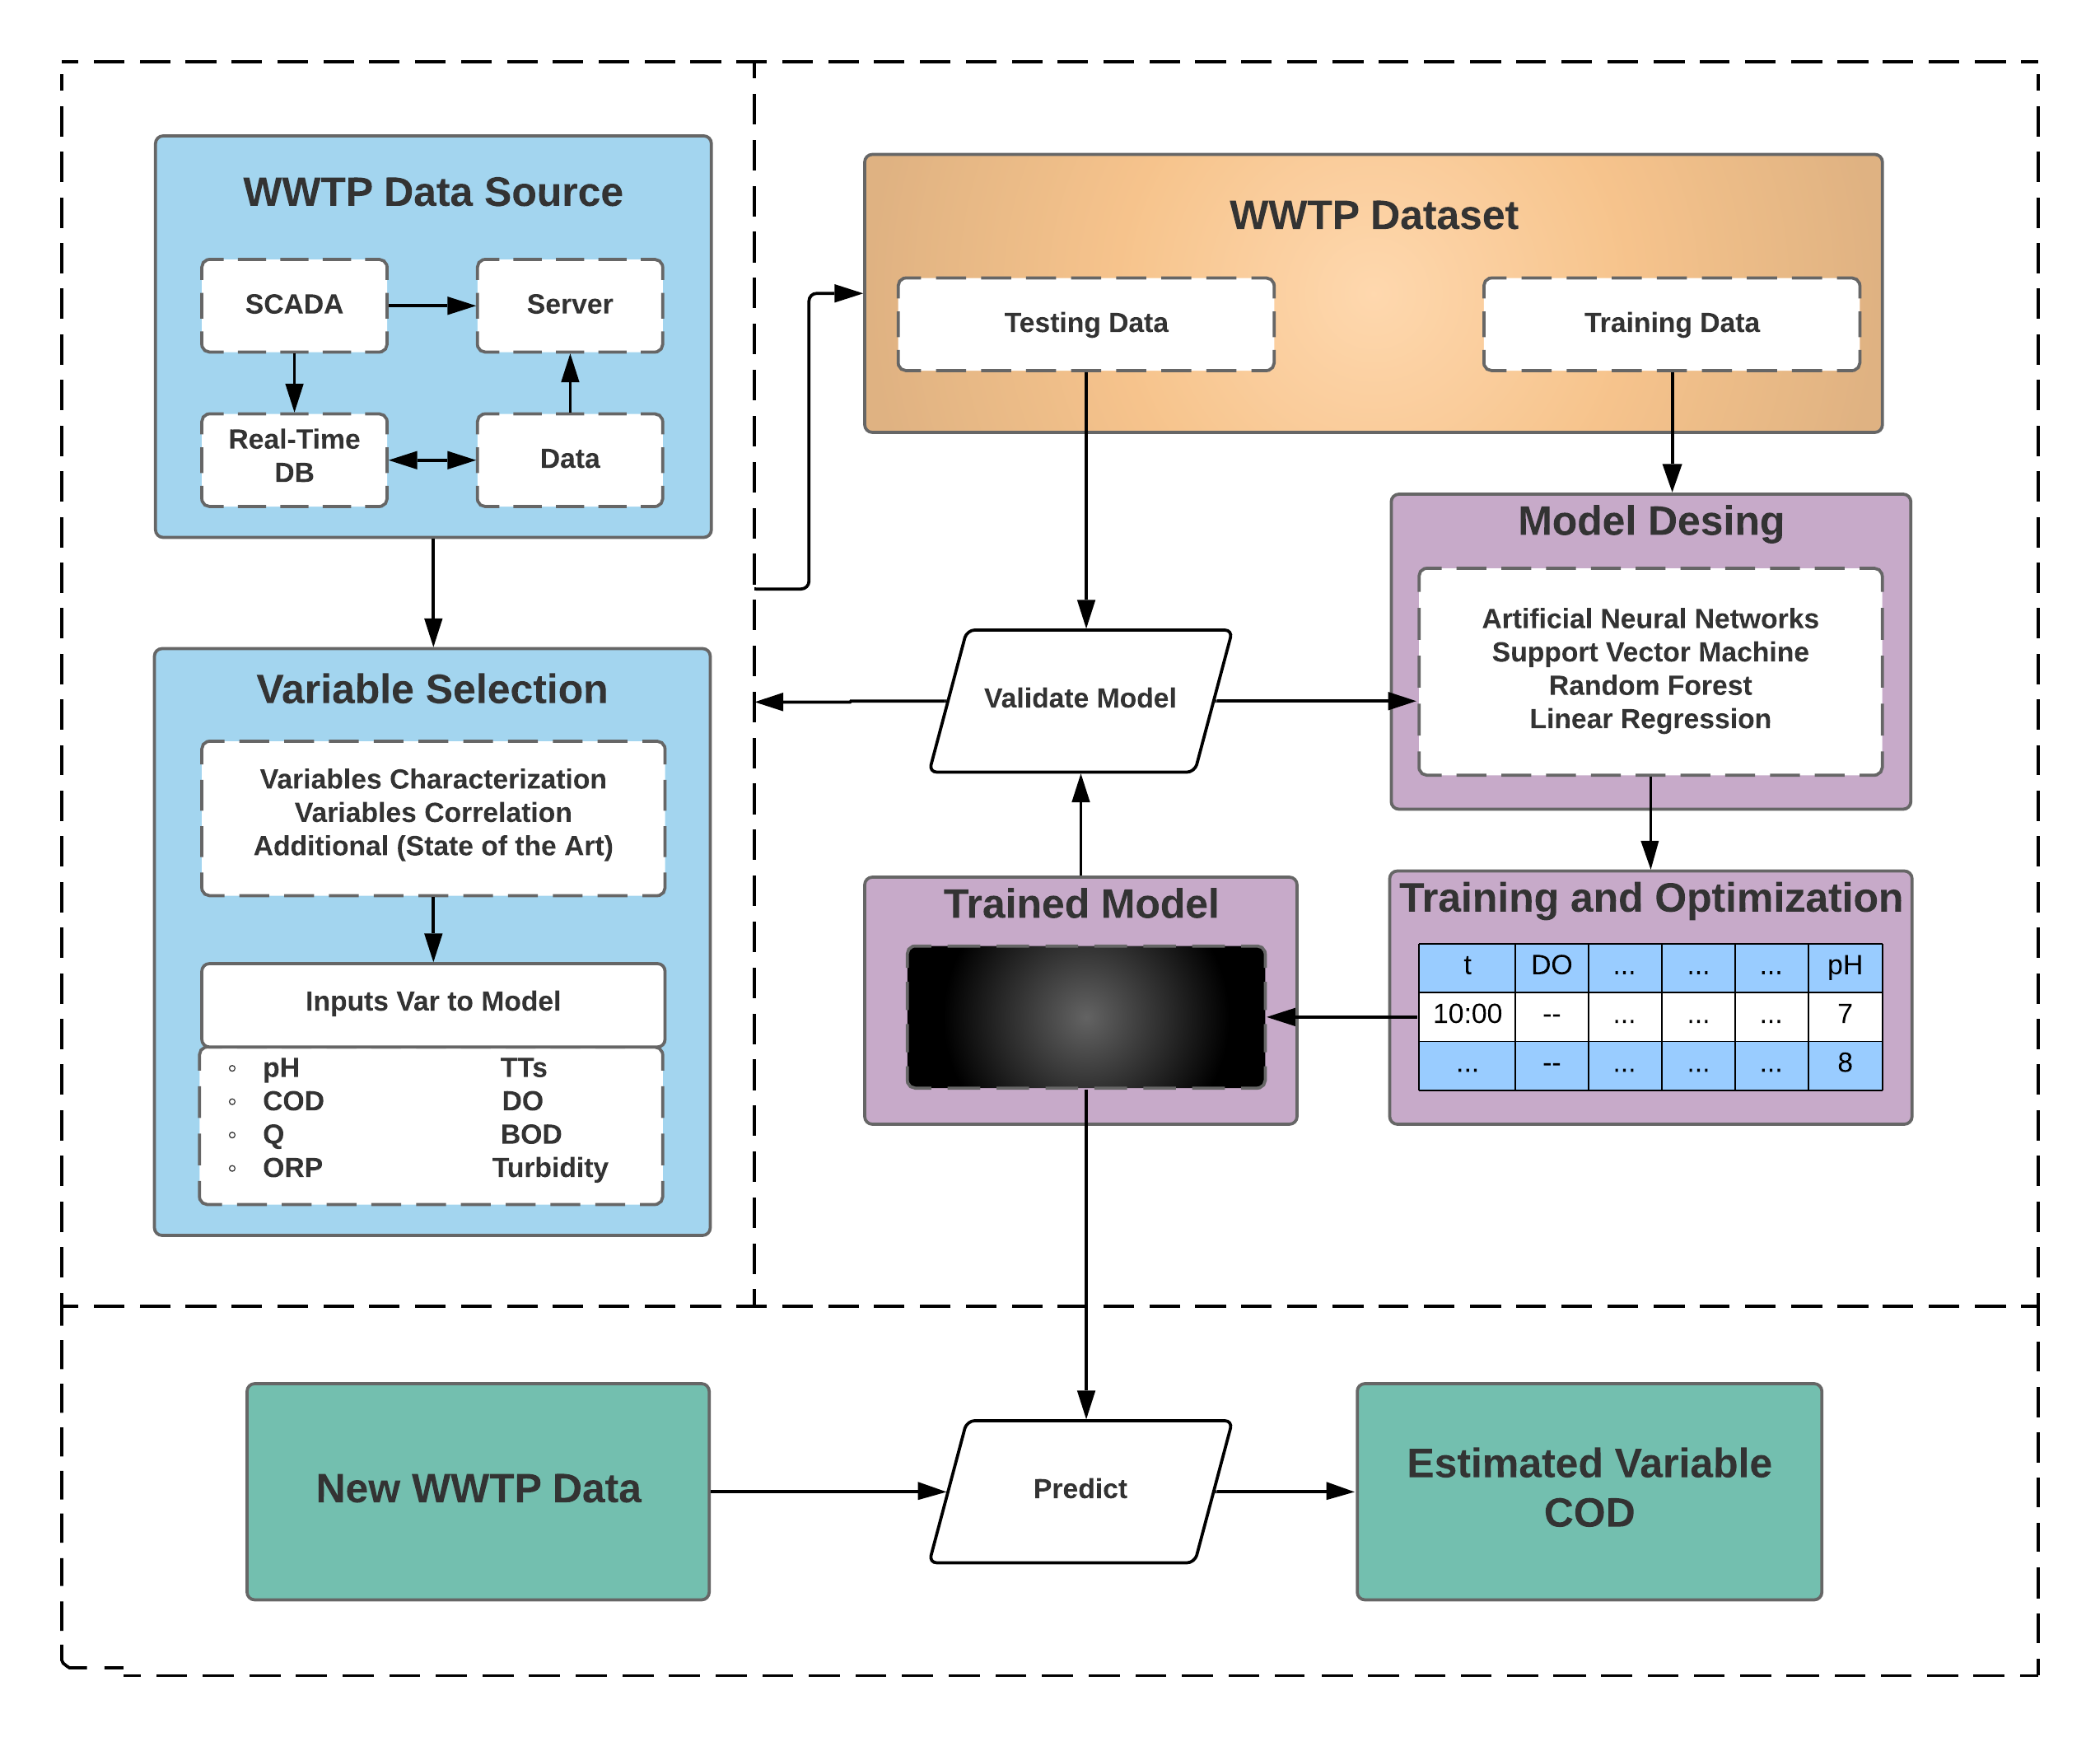
\includegraphics[width=\linewidth]{figures/Ch4/training-FlowChart.png}
\caption{Traininf flow chart}
\label{f:training-flowchart}
\end{figure}

\section{Approach 1}
\label{s:Approach1}

\autoref{f:Approach 1} shows in more detail how the model is conceived and how the COD forecasting is achieved. First, the objective variable taken from the dataset is studied using a time-series decomposition technique that transforms the variable into three additive components: trend, seasonality and residual. Leveraging an auto correlation study over the components, the first two are estimated using their past values. On the other hand, the residual component is estimated using an ANN, which received exogenous variables selected from a correlation study and a past value of the same component. Finally, the addition of the three components provides the COD prediction. 

\begin{figure}[h]
\centering
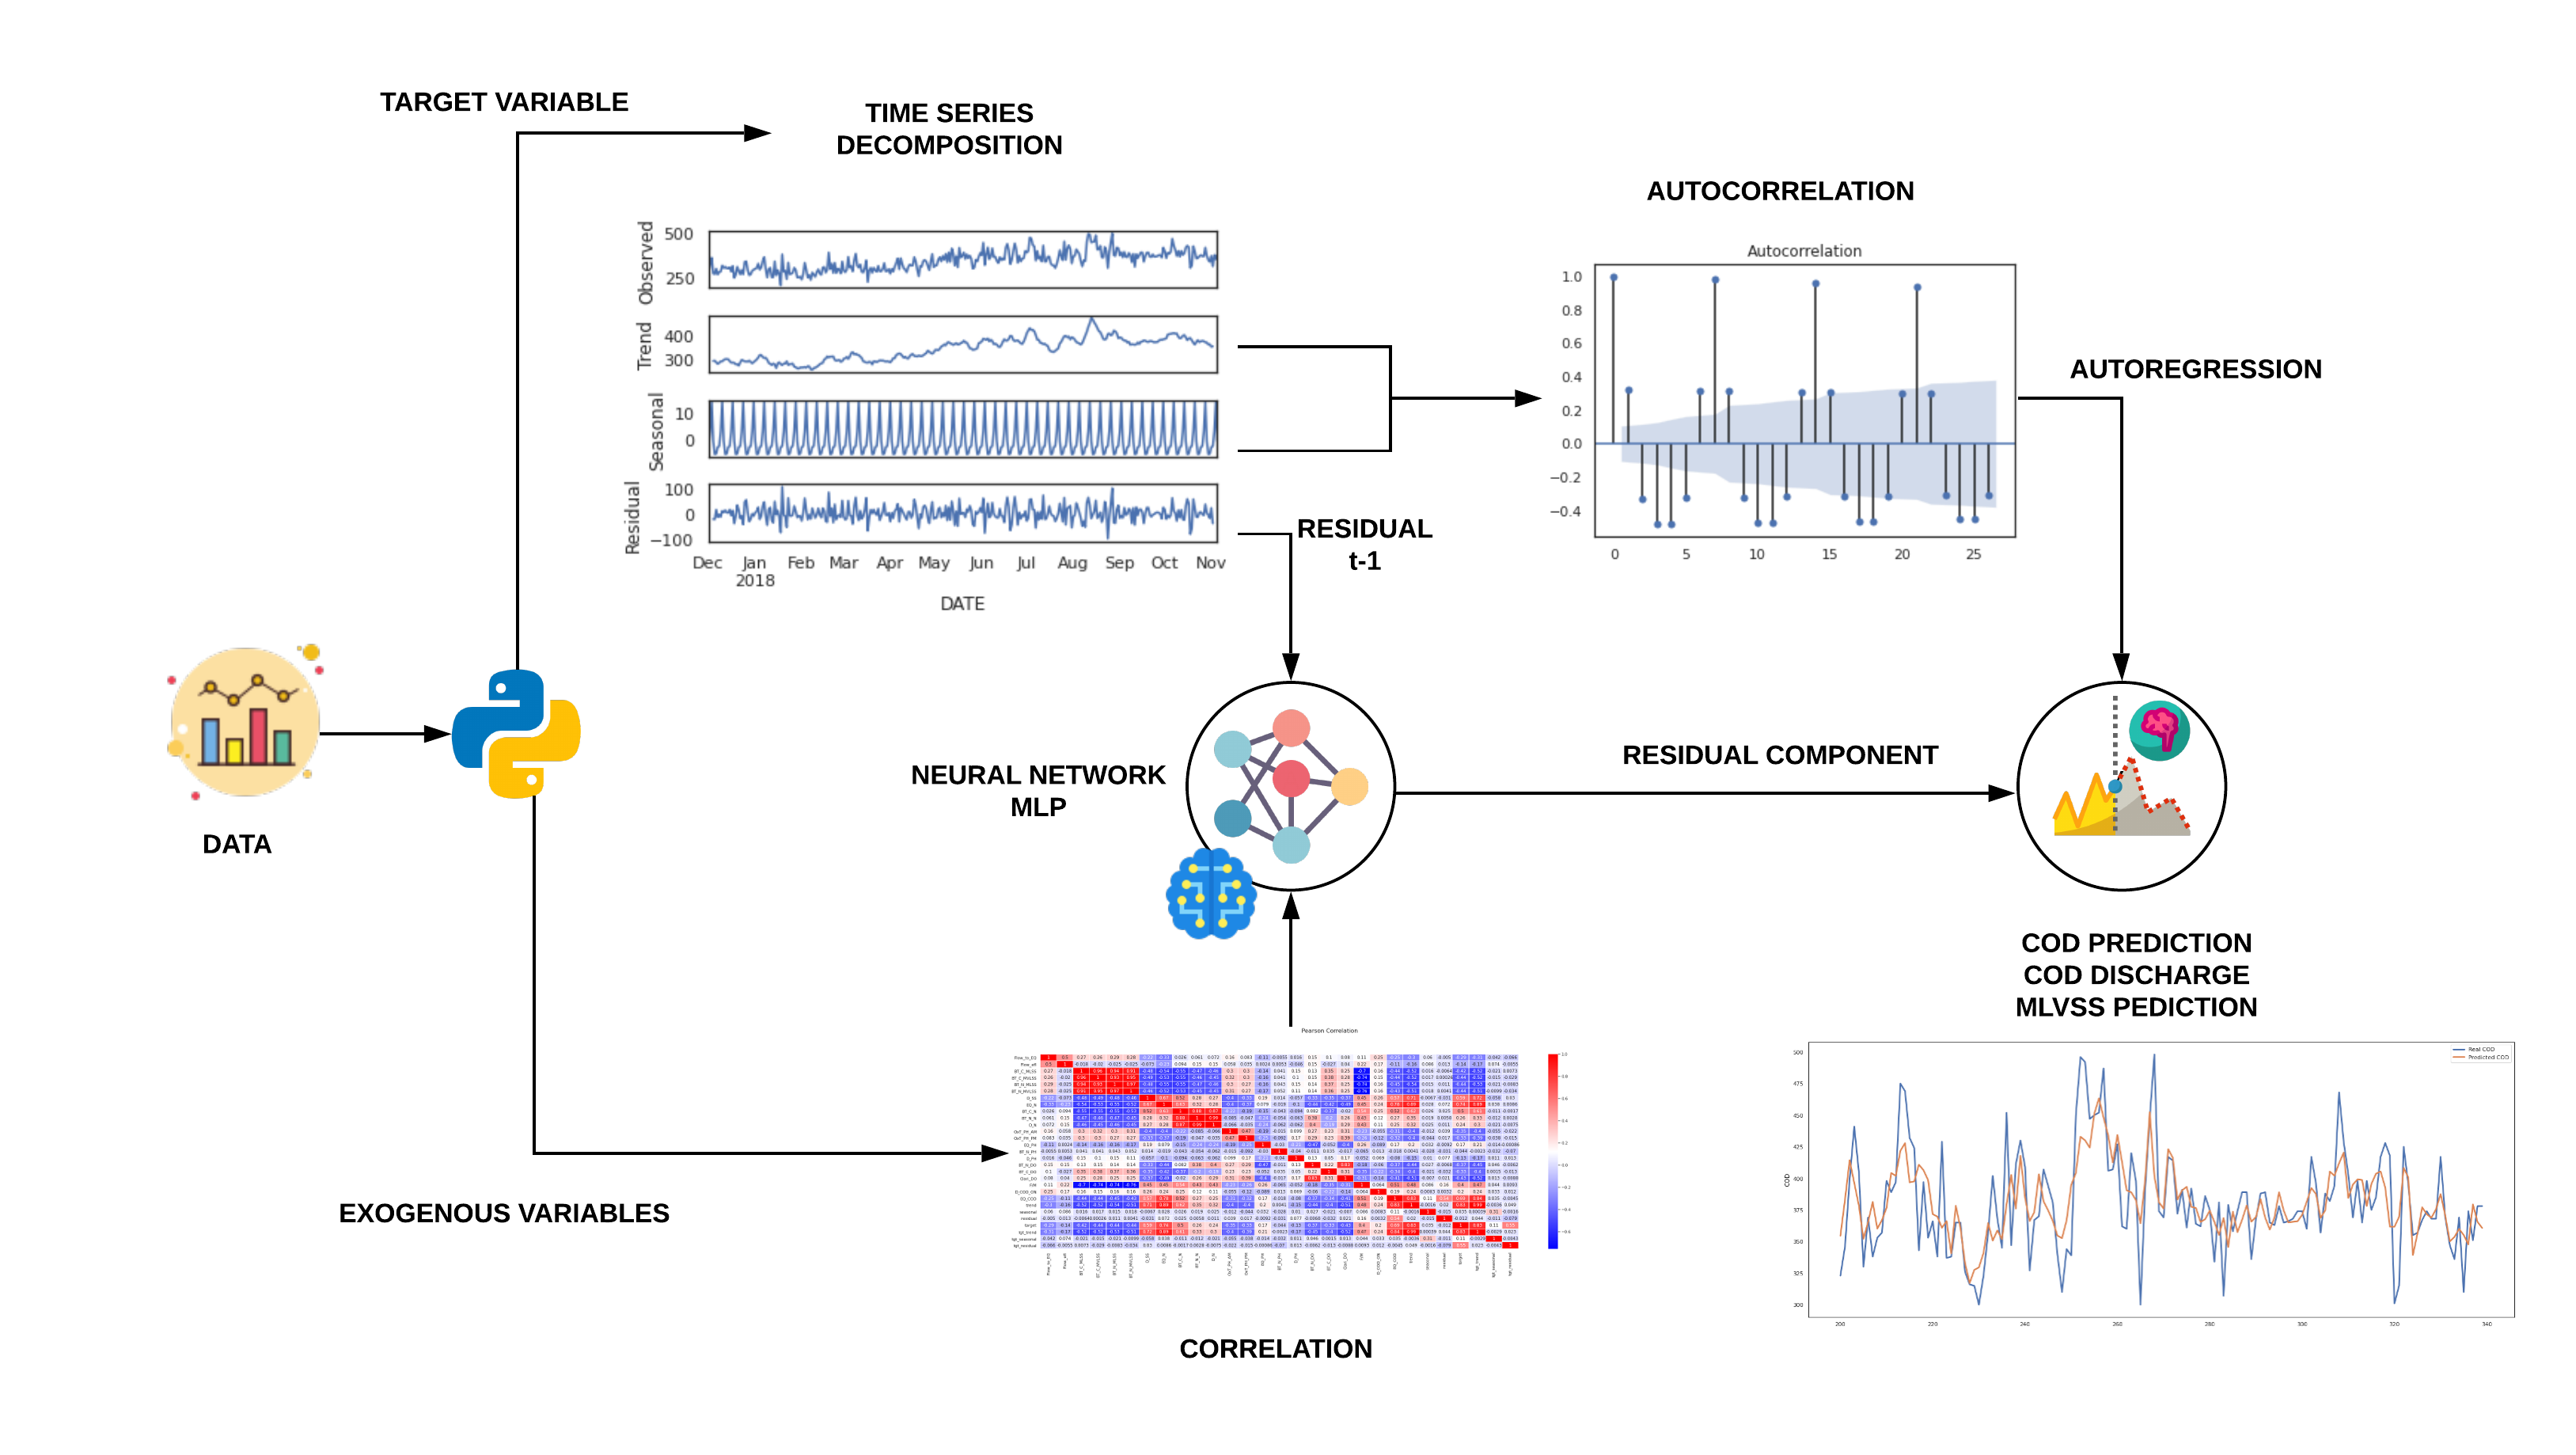
\includegraphics[width=\linewidth]{figures/Ch4/Approach1.png}
\caption{Approach 1}
\label{f:Approach 1}
\end{figure}

\subsection{Time Series Decomposition}
For the time-series analysis of the target, the variable was made a component decomposition where the time series could be represented as a combination of trend, seasonality and residual components [35]. From this point, it was intended to forecast each component of the time series to obtain the objective series using the additive model stated by Pearson and presented in Equation (2) [36], where Tt refers to tendency or trend, St to seasonal movements, Rt to residuals or irregulars and Xt to the series observed.

Figure 7 shows an example of how the equalizer’s COD decomposition looks for the year 2019, where (a) shows the original COD variable, (b) the trend component, (c) the seasonal component and (d) the residual component.

\begin{figure}[h]
\centering
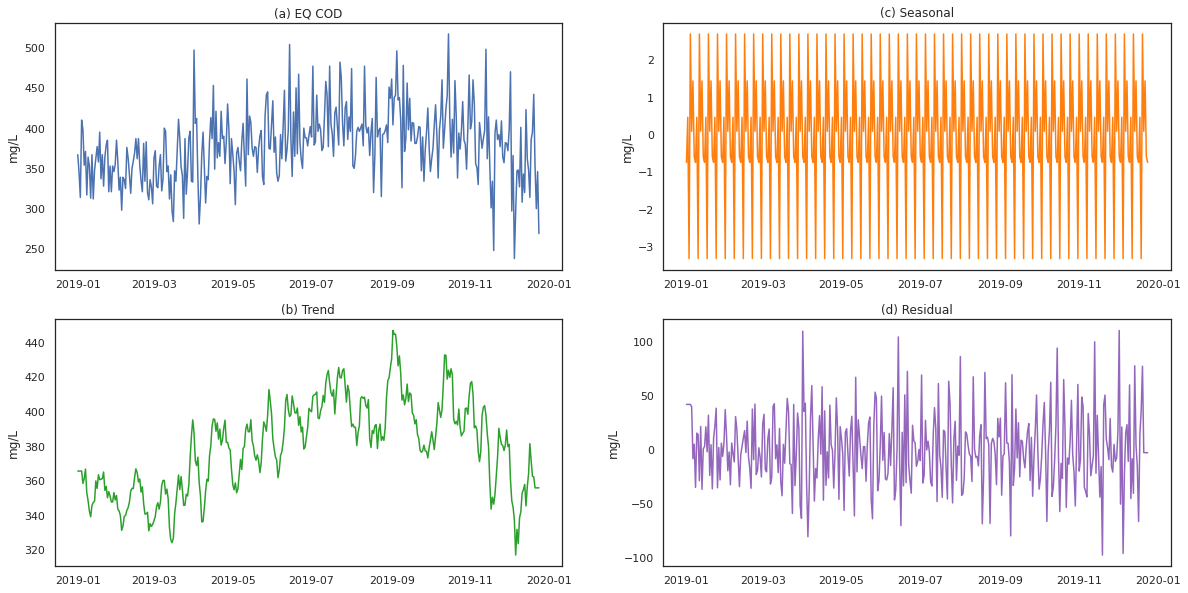
\includegraphics[width=\linewidth]{figures/Ch4/time_series_descompose.png}
\caption{Time Series Decomposition}
\label{f:Time-series-decomposition}
\end{figure}

\subsection{Autocorrelation Study}
Analyzing the time-series decomposition, both autocorrelation and partial autocorrelation studies were made on residual, seasonal and trend COD to extract the important characteristics. From this analysis, it was possible to conduct an autoregressive estimation of the trend and seasonal component of the series. Figures 8, 9, and 10 show the total and partial autocorrelation, respectively. 
\subsection{Model Design}

\newpage
\begin{figure}[h]
\centering
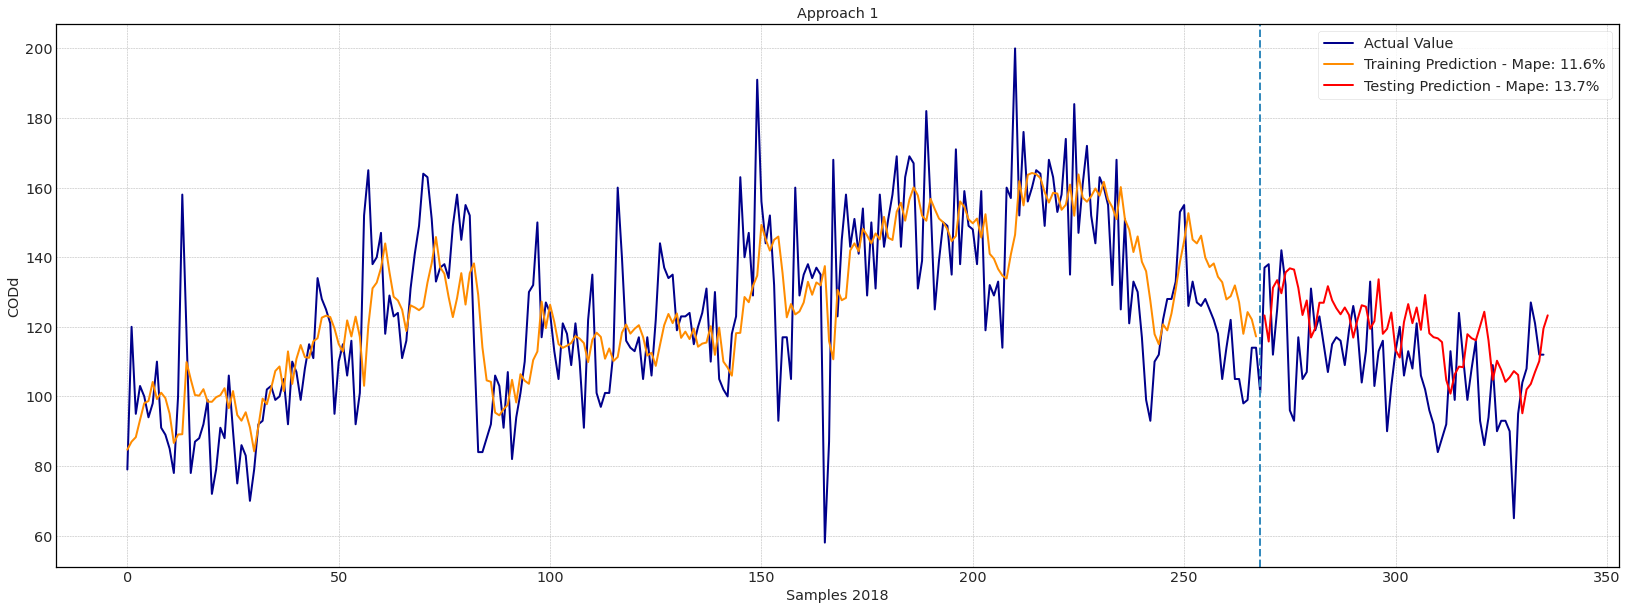
\includegraphics[width=\linewidth]{figures/Ch4/CODd-1.png}
\caption{Approach 1 - CODD}
\label{f:App1-codd}
\end{figure}

\begin{figure}[h]
\centering
\includegraphics[width=\linewidth]{figures/Ch6/CODeq-1.png}
\caption{Approach 1 - CODEQ}
\label{f:App1-codeq}
\end{figure}

\begin{figure}[h]
\centering
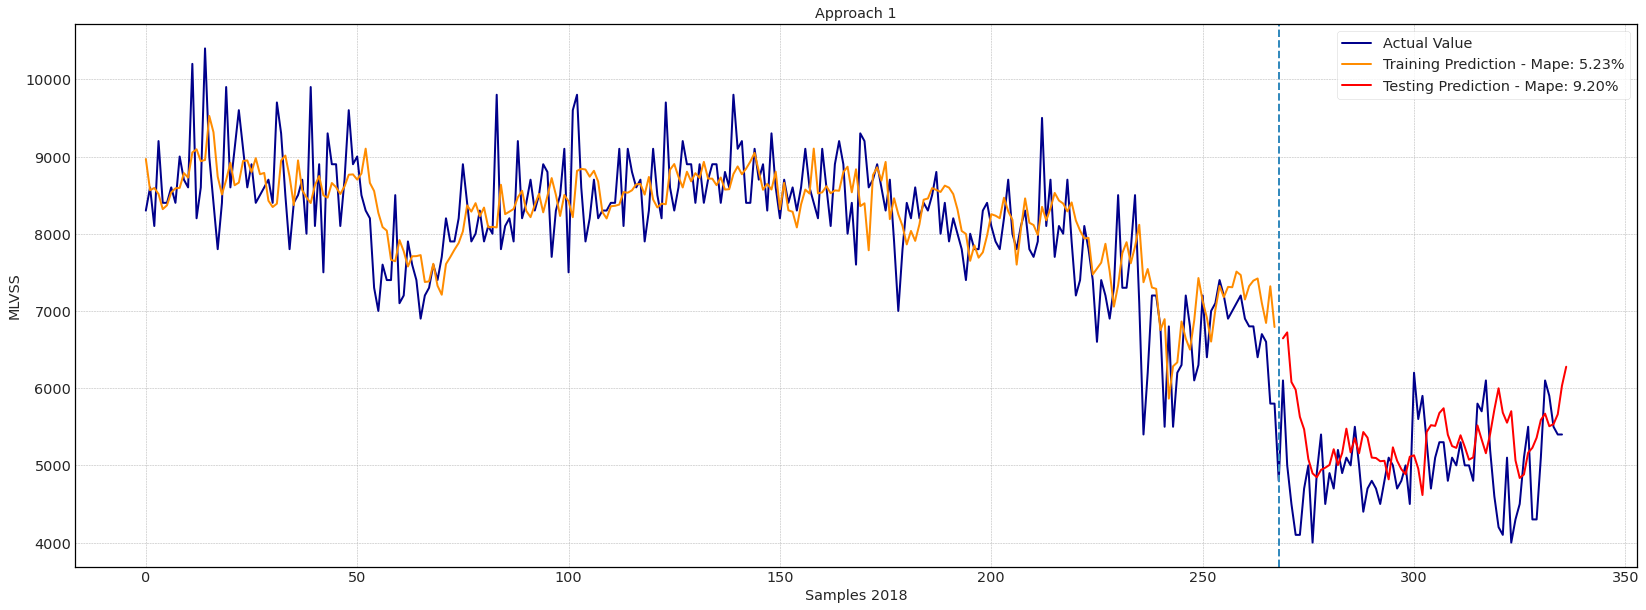
\includegraphics[width=\linewidth]{figures/Ch4/MLVSS-1.png}
\caption{Approach 1 - MLVSS}
\label{f:App1-MLVSS}
\end{figure}

\section{Approach 2}
\label{s:Approach2}

The second approach uses a recurrent neural network, specifically a Long Short-Term Memory (LSTM), a powerful network architecture for sequential data which considers the effect of past values of both endogenous and exogenous variables by itself and learns possible time patterns during the training. Fig. 5 shows a general overview of the second approach. This network requires some data pre-processing to structure the data in sequences format (seven past steps are considered for this study), but nothing more than standardization is applied. 

\begin{figure}[h]
\centering
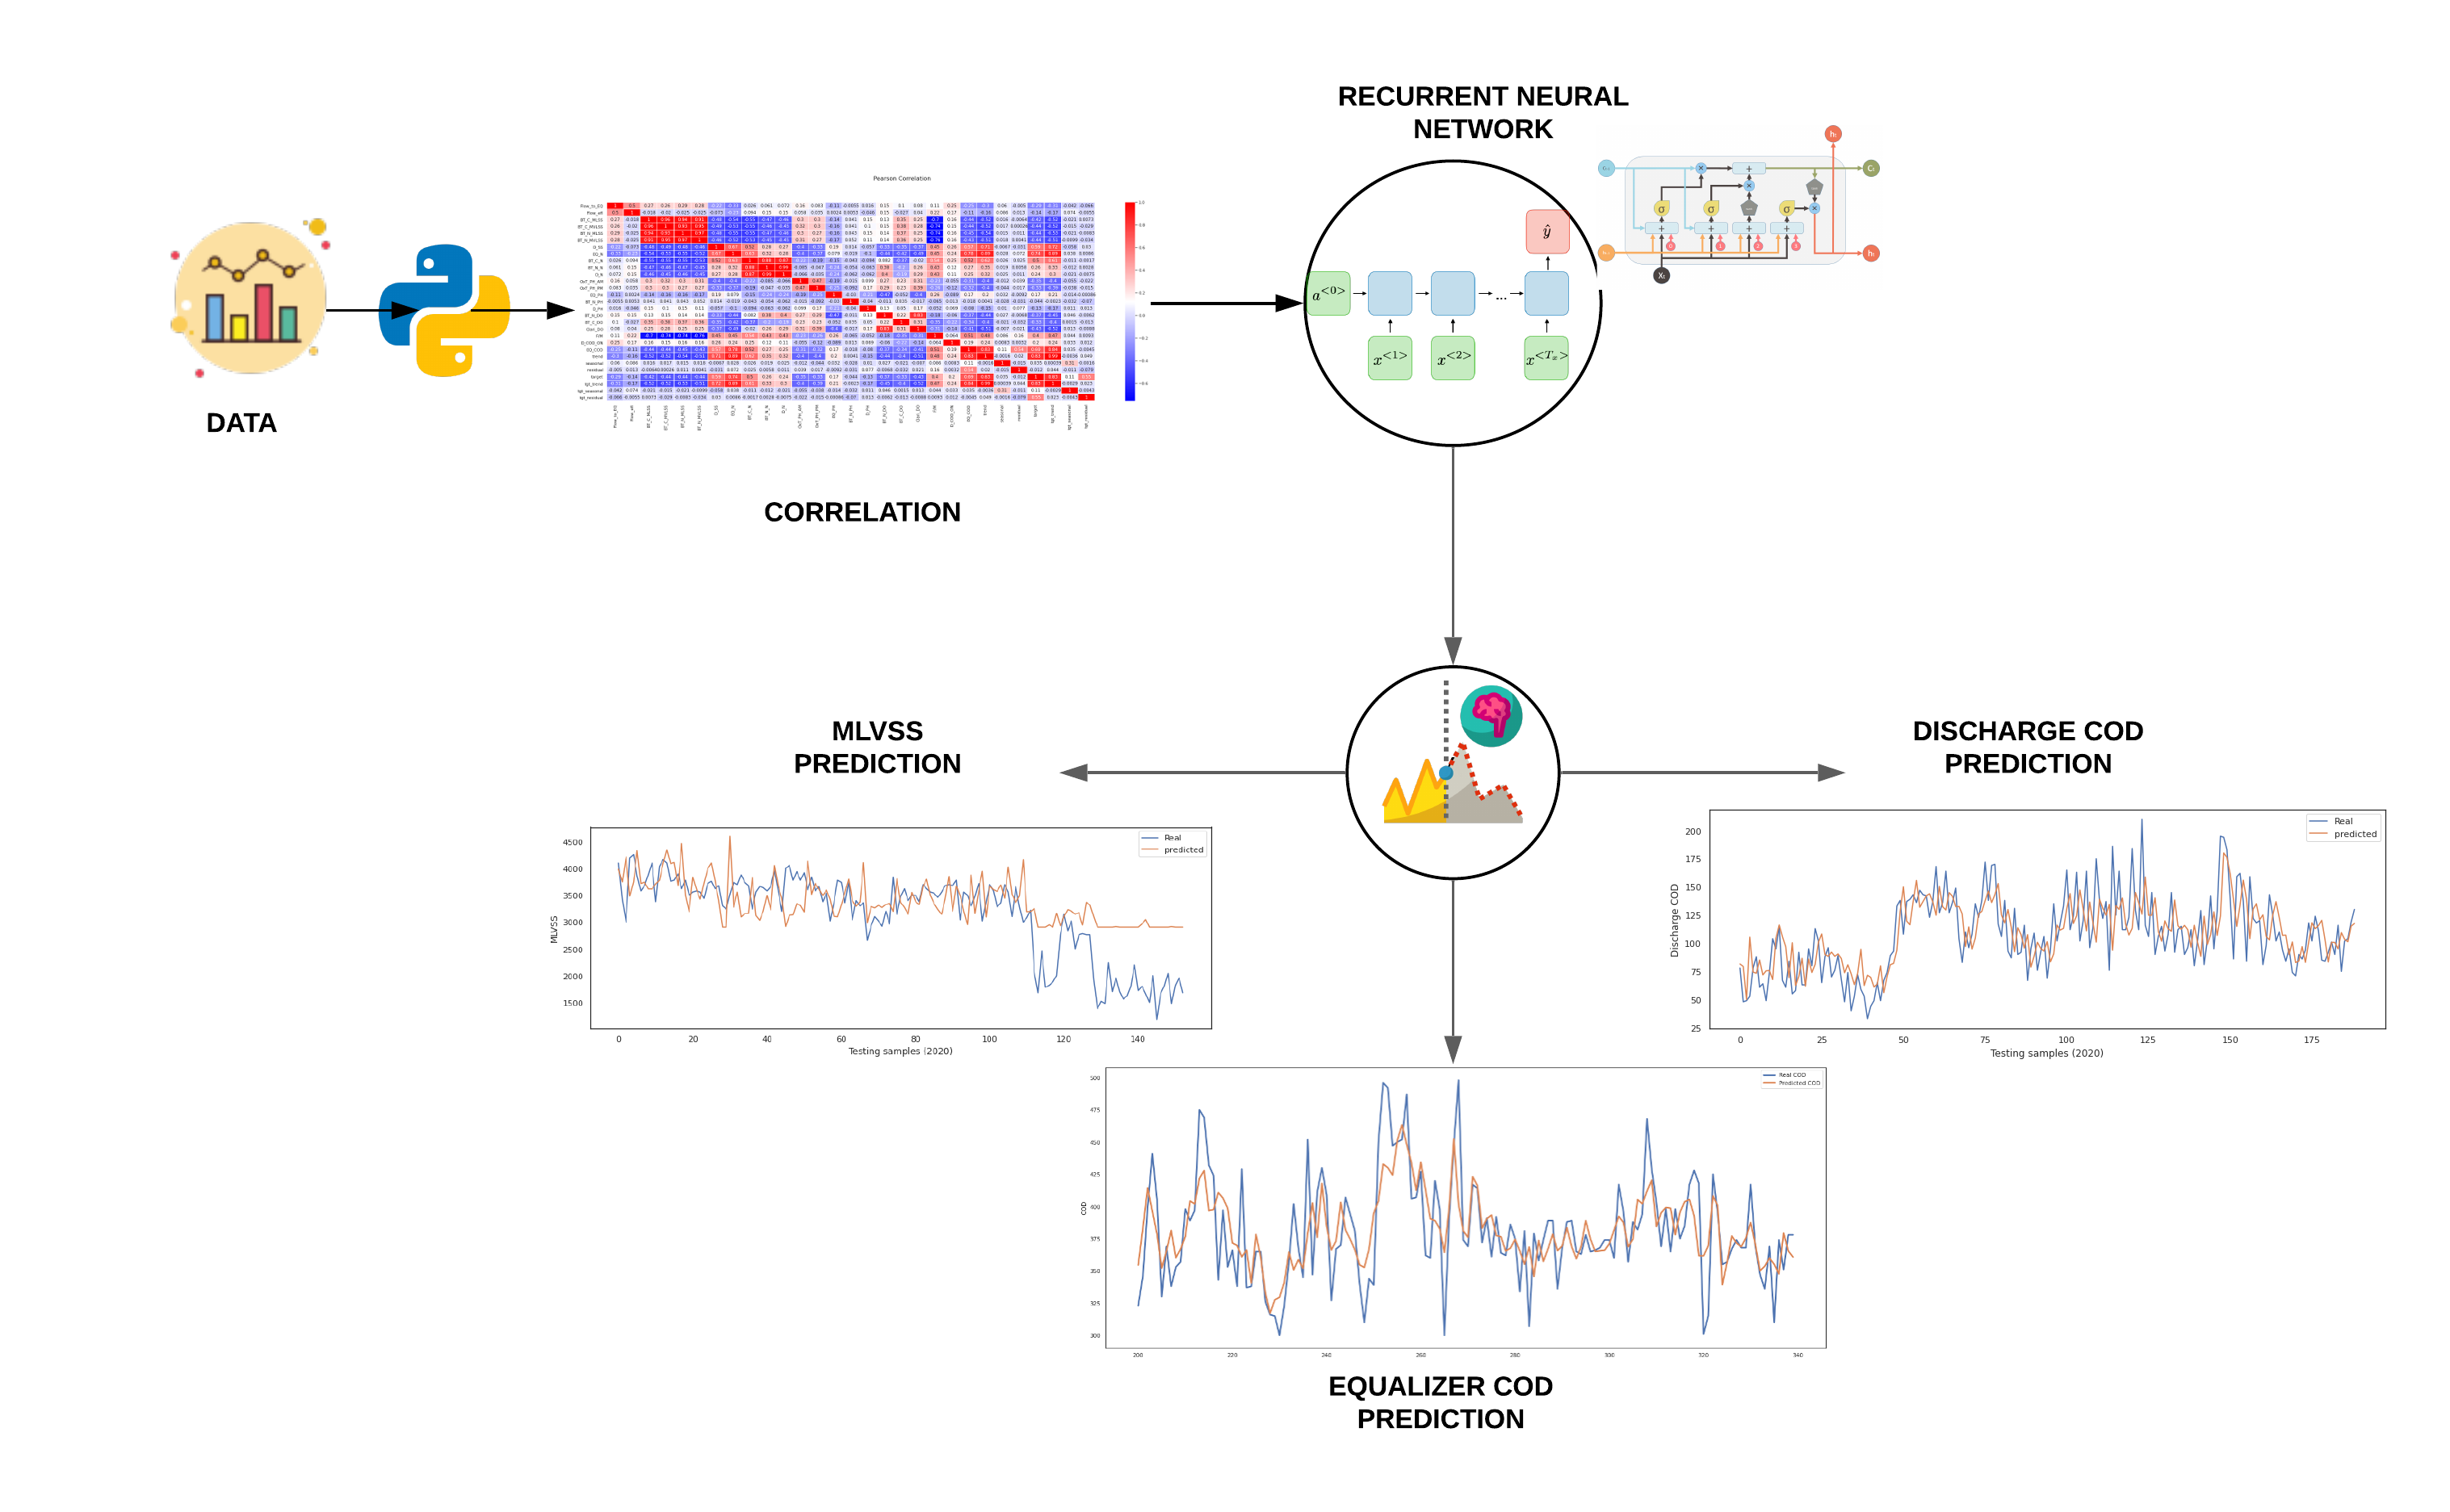
\includegraphics[width=\linewidth]{figures/Ch4/Approach2.png}
\caption{Approach 2}
\label{f:Approach 2}
\end{figure}

\begin{figure}[h]
\centering
\includegraphics[width=\linewidth]{figures/Ch6/CODd-2.png}
\caption{Approach 2 - CODD}
\label{f:App2-codd}
\end{figure}

\begin{figure}[h]
\centering
\includegraphics[width=\linewidth]{figures/Ch6/CODeq-2.png}
\caption{Approach 2 - CODEQ}
\label{f:App2-codeq}
\end{figure}

\begin{figure}[h]
\centering
\includegraphics[width=\linewidth]{figures/Ch6/MVLSS-approach2.png}
\caption{Approach 2 - MLVSS}
\label{f:App2-MLVSS}
\end{figure}

\section{Approach 3}
\label{s:Approach3}

The third approach proposed uses a machine learning technique based on Support Vector Machines. The Support Vector Regression (SVR) algorithm offers an accurate prediction of the time series. This model receives as inputs the exogenous variables selected from the correlation analysis. The implemented model uses Radial Base Function (RBF) kernel, gamma of 0.001, epsilon equal to 0.2 and c value of 10.

\begin{figure}[h]
\centering
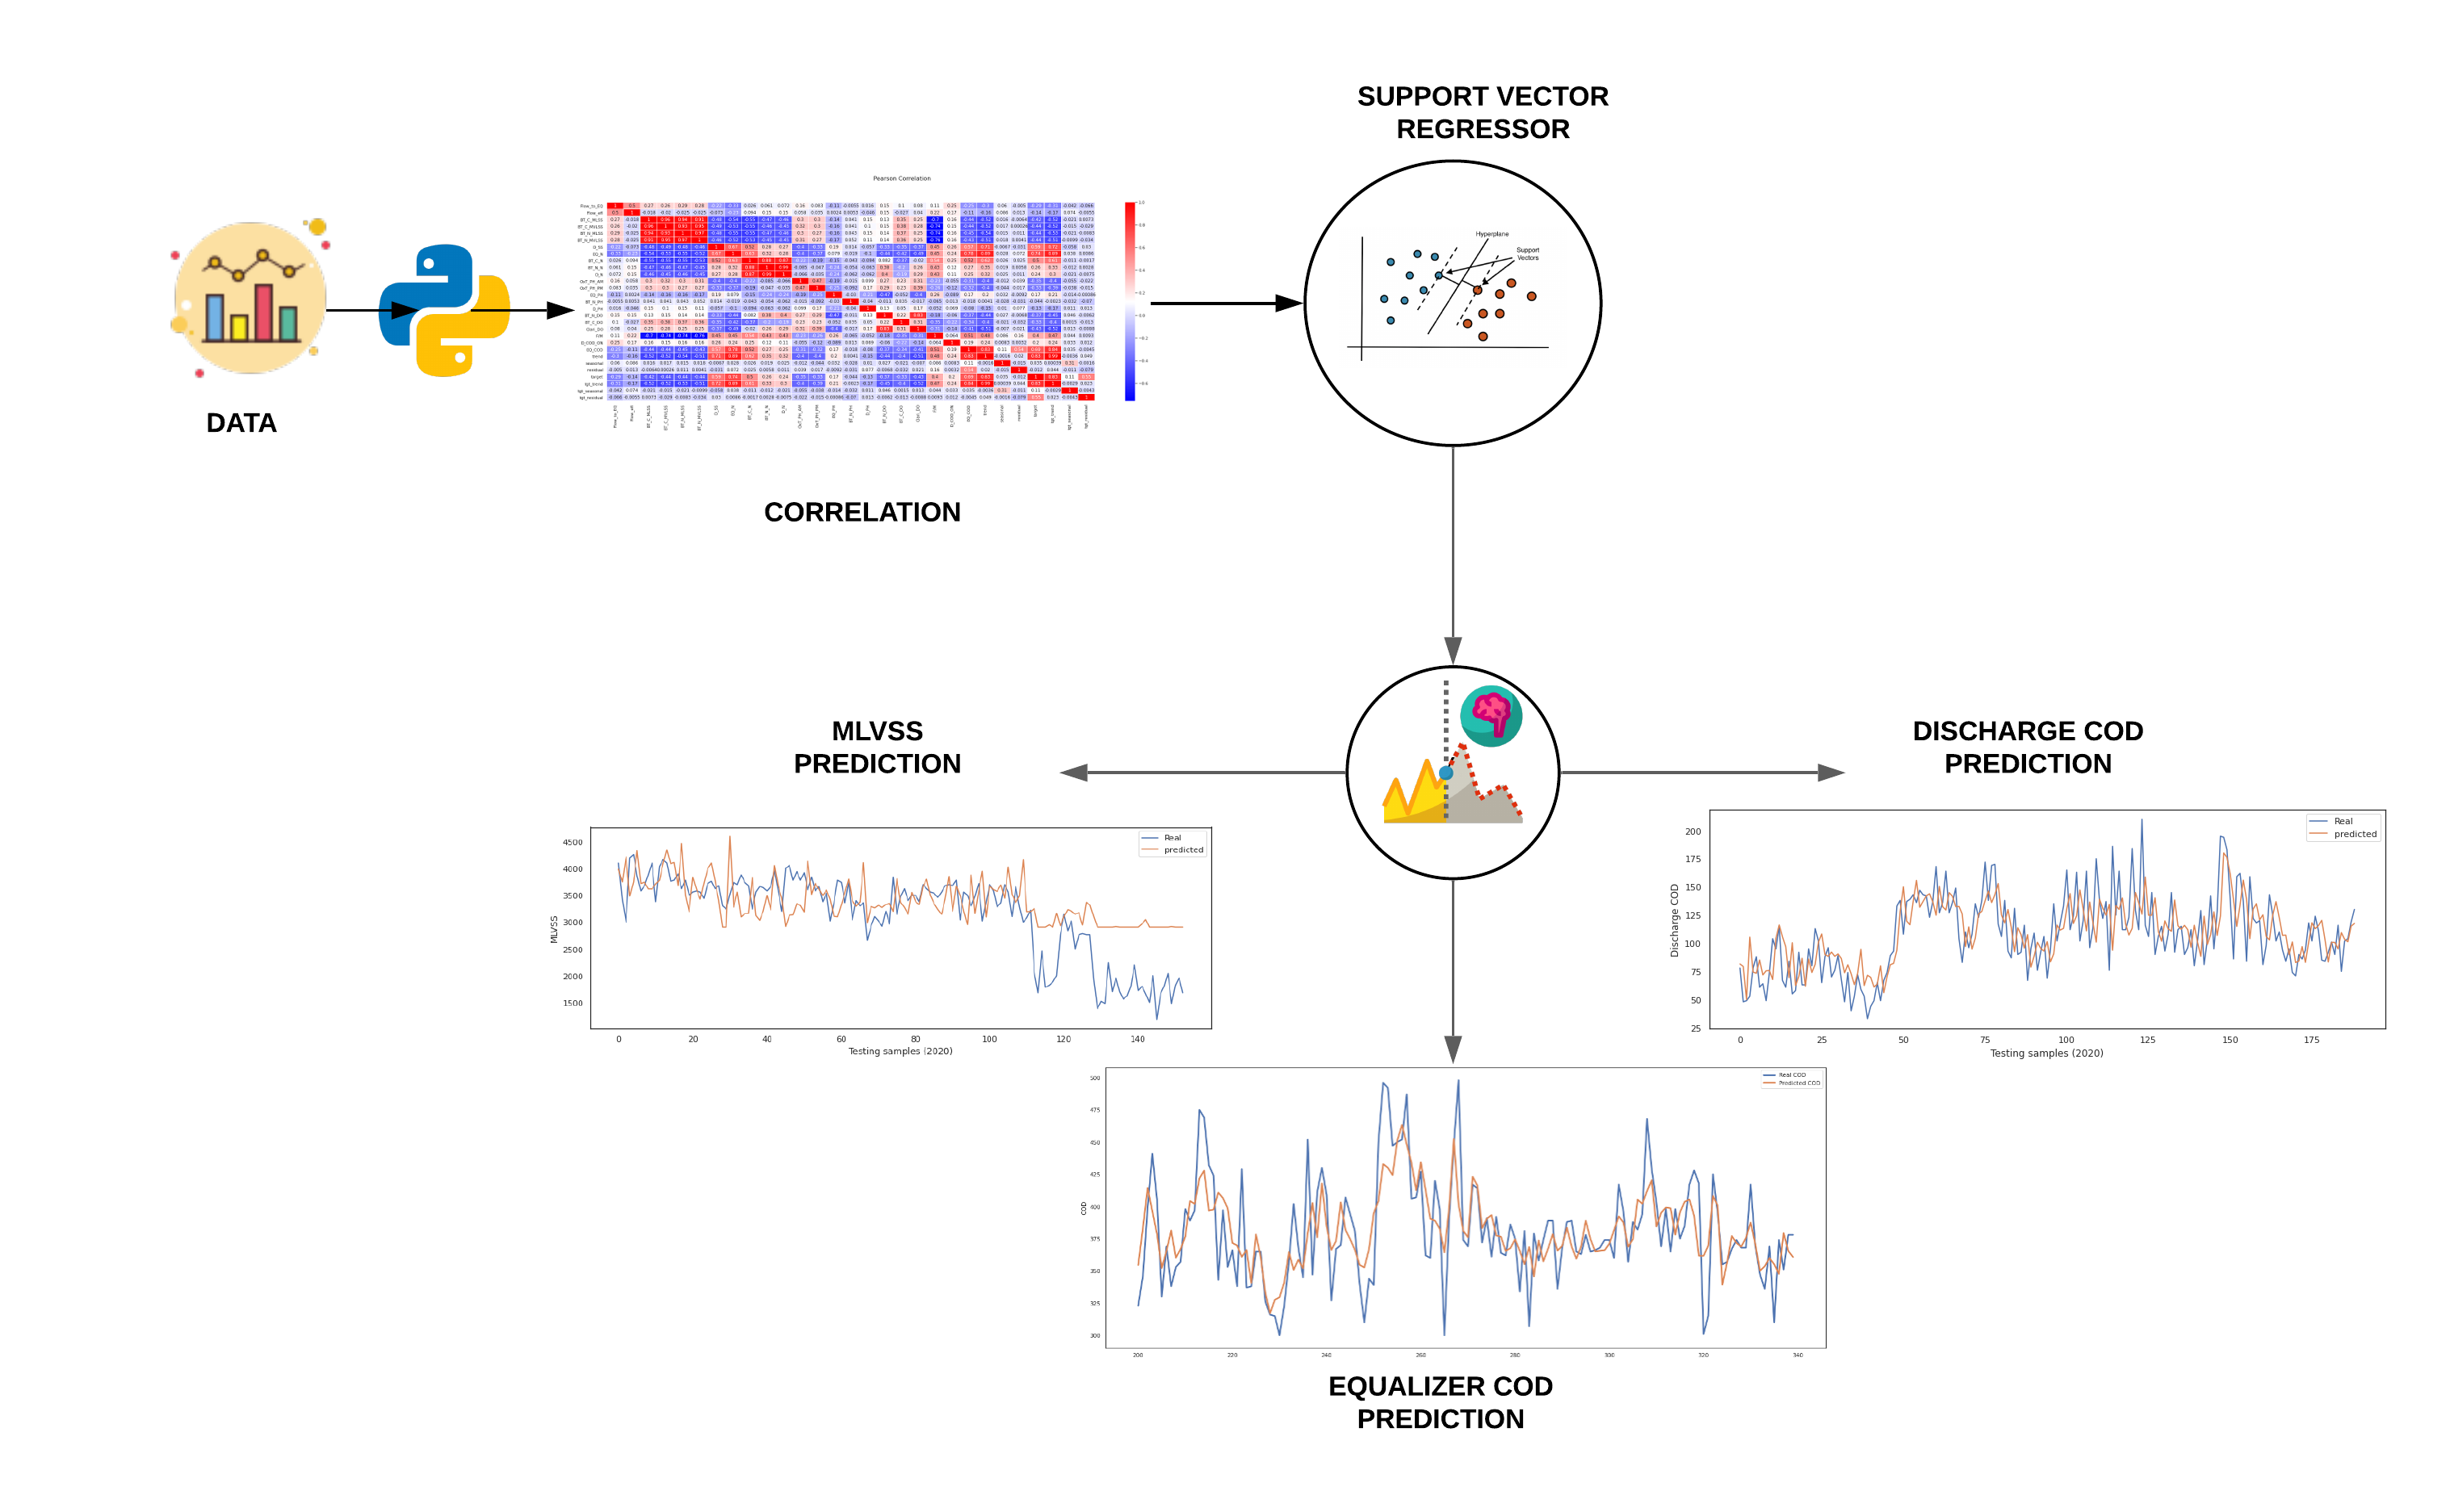
\includegraphics[width=\linewidth]{figures/Ch4/Approach3.png}
\caption{Approach 3}
\label{f:Approach 3}
\end{figure}

\begin{figure}[h]
\centering
\includegraphics[width=\linewidth]{figures/Ch6/CODd-3.png}
\caption{Approach 3 - CODD}
\label{f:App3-codd}
\end{figure}

\begin{figure}[h]
\centering
\includegraphics[width=\linewidth]{figures/Ch6/CODeq-3.png}
\caption{Approach 3 - CODEQ}
\label{f:App3-codeq}
\end{figure}

\begin{figure}[h]
\centering
\includegraphics[width=\linewidth]{figures/Ch6/MVLSS-approach3.png}
\caption{Approach 3 - MLVSS}
\label{f:App3-MLVSS}
\end{figure}


\section{Summary}
\label{s:Contribution-1-Summary}

The final section of each major chapter should summarize the chapter. In comparison to the chapter, the summary should be short ($\frac{1}{2}$ to $2$ pages is normal).
  
  \chapter{Major Contribution 2}\label{c:Contribution-2}
  This chapter presents the results of the proposed approaches implementation. Additional details of the models are presented and their performance over training and testing data. 

\section{Variables Selection}
\label{s:results_data_selection}

The Pearson correlation is calculated to select the optimal input variables for the system. \autoref{t:correlation_table} summarizes the correlation values for the three target variables where \ac{COD}\textsubscript{D}, \ac{COD}\textsubscript{EQ}, and \ac{MLVSS} are one-day a head shifted variables.

%\begin{longtable}{@{}l *{2}{rr}}
\begin{longtable}[h!]{@{}l *{2}{rr}}
\caption[Portrait Table, short caption]{Variables Correlation}
\label{t:correlation_table}
\\
%   
\toprule%


 {\bfseries Variable} & {\bfseries COD\textsubscript{D} } & {\bfseries COD\textsubscript{EQ}} & {\bfseries MLVSS}
\\

\cmidrule[0.4pt](r{0.125em}){1-1}%
\cmidrule[0.4pt](lr{0.125em}){2-4}%
%\cmidrule[0.4pt](lr{0.125em}){4-5}%
%\cmidrule[0.4pt](lr{0.125em}){5-6}%


  \endfirsthead

\endhead

        Flow\_to\_EQ & 0.14 & -0.14 & -0.025  \\ 
        BT\_C\_MLSS & 0.11 & -0.43 & 0.88  \\ 
        BT\_C\_MLVSS & 0.10 & -0.45 & 0.9  \\ 
        BT\_N\_MLSS & 0.10 & -0.44 & 0.88  \\ 
        BT\_N\_MLVSS & 0.10 & -0.44 & 0.88  \\ 
        D\_SS & 0.3 & 0.59 & -0.46  \\ 
        EQ\_N & 0.25 & 0.74 & -0.54  \\ 
        BT\_C\_N & 0.25 & 0.49 & -0.54  \\ 
        BT\_N\_N & 0.11 & 0.26 & -0.47  \\ 
        D\_N & 0.11 & 0.23 & -0.46  \\ 
        OxT\_pH & -0.12 & -0.33 & 0.27  \\ 
        EQ\_pH & -0.069 & 0.18 & -0.17  \\ 
        BT\_N\_pH & 0.057 & -0.045 & 0.083  \\ 
        D\_pH & 0.059 & -0.13 & 0.078  \\ 
        BT\_N\_DO & -0.1 & -0.37 & 0.14  \\ 
        BT\_C\_DO & -0.28 & -0.33 & 0.34  \\ 
        Clari\_DO & -0.17 & -0.43 & 0.27  \\ 
        ST\_COD & 0.22 & 0.63 & -0.44  \\ 
        D\_COD\_ON & 0.72 & 0.22 & 0.11  \\


\bottomrule

\end{longtable}

Variables that present a correlation higher than 0.2 are selected as inputs for the system. As a result the input variables for each target variable are presented below:

\begin{itemize}
    \item \textbf{COD\textsubscript{D} :} D\_SS, BT\_C\_N, EQ\_N, BT\_C\_DO, ST\_COD, EQ\_COD, D\_COD\_ON.
    \item \textbf{COD\textsubscript{EQ} :} BT\_C\_MVLSS, D\_SS, EQ\_N, BT\_C\_N, OxT\_PH\_PM, BT\_N\_DO, Clari\_DO, ST\_COD, EQ\_COD.
    \item \textbf{MLVSS :} BT\_C\_MVLSS, D\_SS, EQ\_N, BT\_C\_N, OxT\_PH\_PM, BT\_C\_DO, Clari\_DO, ST\_COD, EQ\_COD.
\end{itemize}

It results necessary standardize this variables in order to take them to similar level values. This step helps the model to give the same level of relevance to each input variable no matter what its magnitude value is.

\begin{equation}
    X'_i = \frac{x_i - x_{mean}}{x_{std}}
\end{equation}

\begin{itemize}
    \item \begin{math}X'_i\end{math} is each standardized value.
    \item \begin{math}X_i\end{math} is each raw value.
    \item \begin{math}X_{mean}\end{math} is the mean value of the variable in the training dataset.
    \item \begin{math}X_{std}\end{math} is the standard deviation value of the variable in the training dataset.
\end{itemize}


\section{Approach 1}
\label{s:resutls-approach1}
The first approach conducts the time series decomposition just as described in \autoref{ss:time-series-decomposition} for each target variable. It estimates the trend and seasonal components by applying auto-regression of its past values, process supported in the auto-correlation study just as mentioned in \autoref{ss:autocorrelation}. The residual component is predicted by a \ac{FFNN} that receives the inputs presented in \label{s:results_data_selection} and includes the actual residual value as an additional input feature. The \ac{FFNN} architecture and the approach prediction results are presented bellow.
All model hyper-parameters were tuned by a grid search between following options:

\begin{itemize}
    \item Loss = [mse, mae]
    \item Optimizer = [SGD, adam]
    \item Activation = [linear, tanh]
    \item Number of Layers = [1, 2]
    \item Number of Neurons per layer = [2, 4, 6, 8, 10, 12, 14, 16, 18, 20, 22, 24, 26, 28, 30, 32]
    \item Batch Normalization = [0, 1]
\end{itemize}

\subsection{COD Discharge}
\autoref{f:App1-codd-nn} shows the structure of the \ac{FFNN} used for \ac{COD}\textsubscript{D} residual prediction which hyper-parameters are presented below. \autoref{f:App1-codd} shows the prediction results of this approach where the orange line corresponds to model prediction over the training data, the red line to the model prediction over the testing samples and finally the blue one indicates the actual value the target variable takes.

\begin{figure}[h]
\centering
 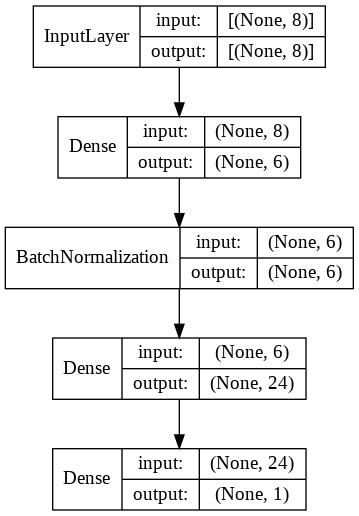
\includegraphics[width=0.4\linewidth]{figures/Ch5/App1_CODeq.png}
\caption{Approach 1 - COD\textsubscript{D} Network}
\label{f:App1-codd-nn}
\end{figure}

\begin{figure}[hb!]
\centering
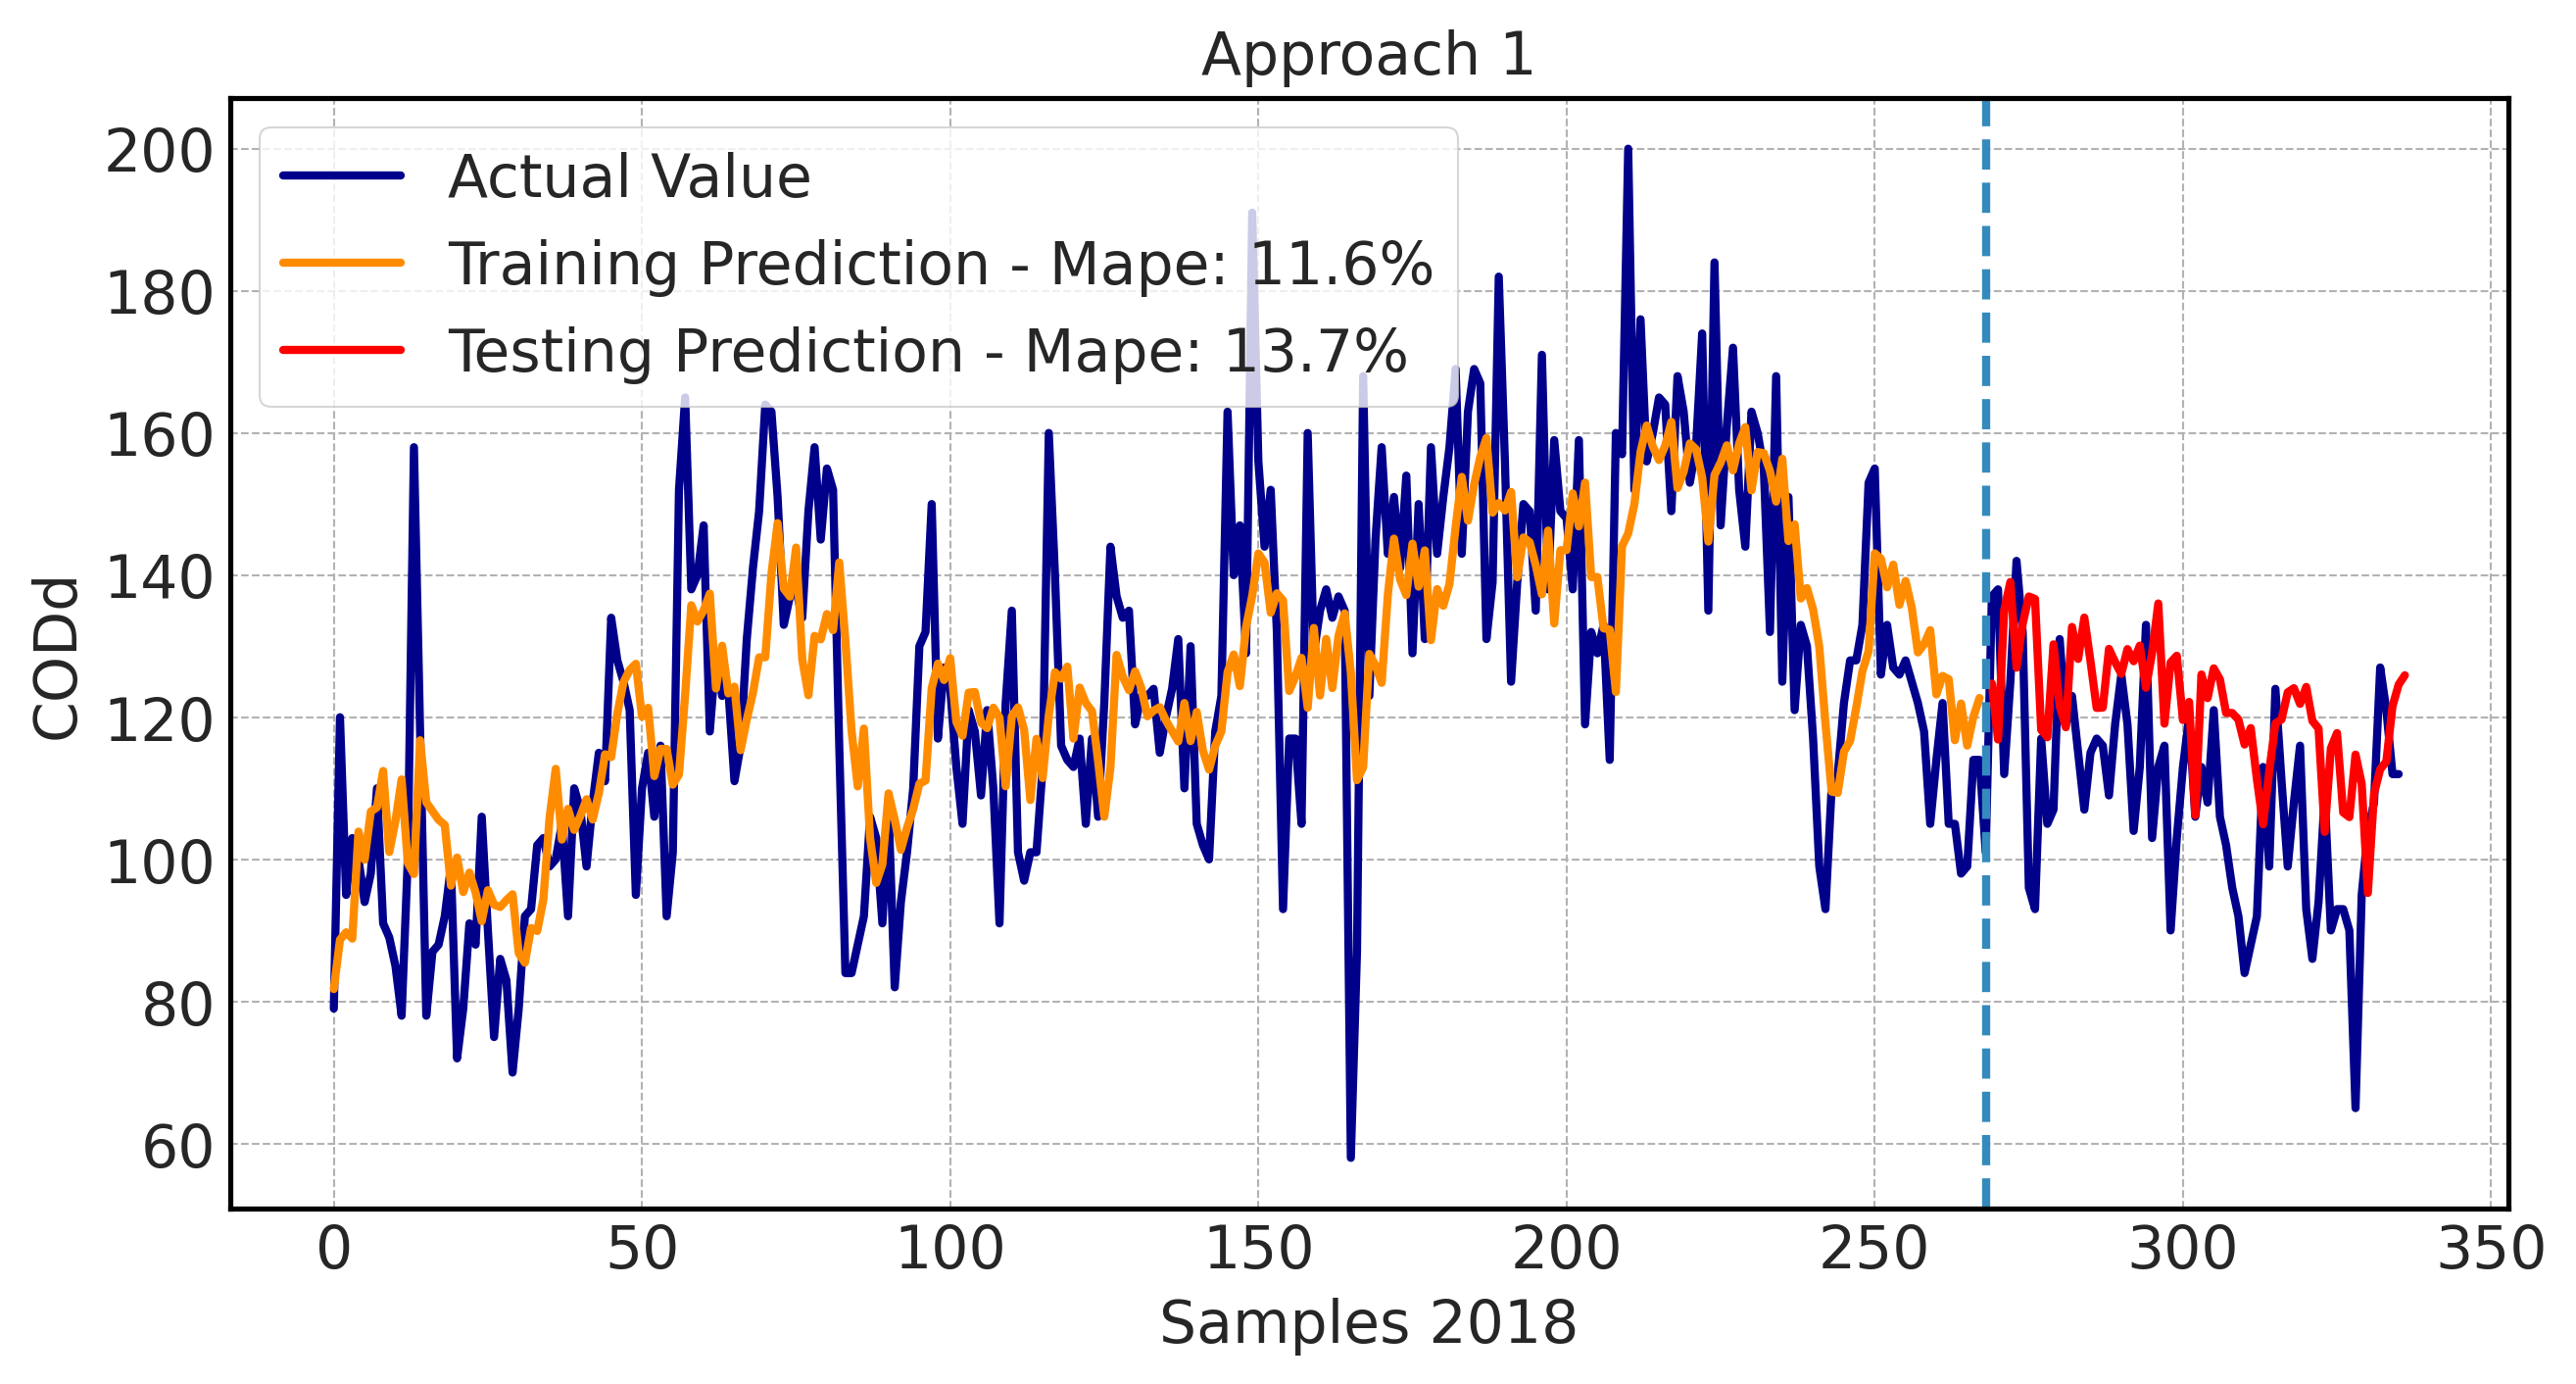
\includegraphics[width=\linewidth]{figures/Ch5/CODd-1.png}
\caption{Approach 1 - COD\textsubscript{D}}
\label{f:App1-codd}
\end{figure}

\begin{itemize}
    \item Loss = mse
    \item Optimizer = SGD
    \item Activation =  tanh
    \item Number of Layers = 2
    \item Number of Neurons per layer = [6, 24]
    \item Batch Normalization = 1
\end{itemize}

\subsection{COD Equalizer}
\autoref{f:App1-codeq-nn} shows the structure of the \ac{FFNN} used for \ac{COD}\textsubscript{EQ} residual prediction which hyper-parameters are presented below. \autoref{f:App1-codd} shows the prediction results of this approach.

\begin{itemize}
    \item Loss = mse
    \item Optimizer = SGD
    \item Activation =  Linear
    \item Number of Layers = 2
    \item Number of Neurons per layer = [10, 18]
    \item Batch Normalization = 1
\end{itemize}

\begin{figure}[h]
\centering
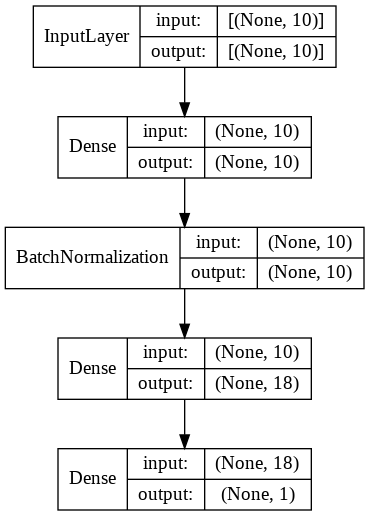
\includegraphics[width=0.4\linewidth]{figures/Ch5/App1_CODd.png}
\caption{Approach 1 - COD\textsubscript{EQ} Network}
\label{f:App1-codeq-nn}
\end{figure}

\begin{figure}[h]
\centering
\includegraphics[width=\linewidth]{figures/Ch5/CODeq-1.png}
\caption{Approach 1 - COD\textsubscript{EQ}}
\label{f:App1-codeq}
\end{figure}

\subsection{MLVSS}

\autoref{f:App1-MLVSS-nn} shows the structure of the \ac{FFNN} used for \ac{MLVSS} residual prediction which hyper-parameters are presented below. \autoref{f:App1-MLVSS} shows the prediction results of this approach.

\begin{figure}[h!]
\centering
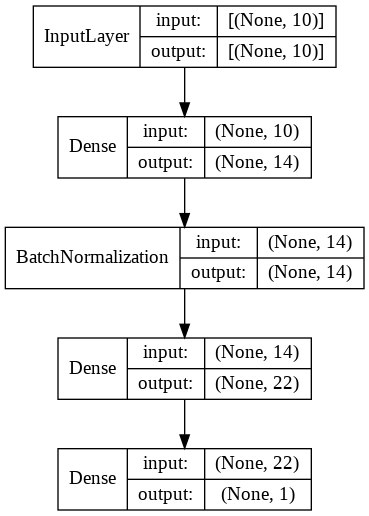
\includegraphics[width=0.4\linewidth]{figures/Ch5/App1_MLVSS.png}
\caption{Approach 1 - MLVSS Network}
\label{f:App1-MLVSS-nn}
\end{figure}

\begin{itemize}
    \item Loss = mse
    \item Optimizer = SGD
    \item Activation =  Relu
    \item Number of Layers = 2
    \item Number of Neurons per layer = [14, 22]
    \item Batch Normalization = 1
\end{itemize}
%------------------------------------------------
\begin{figure}[h]
\centering
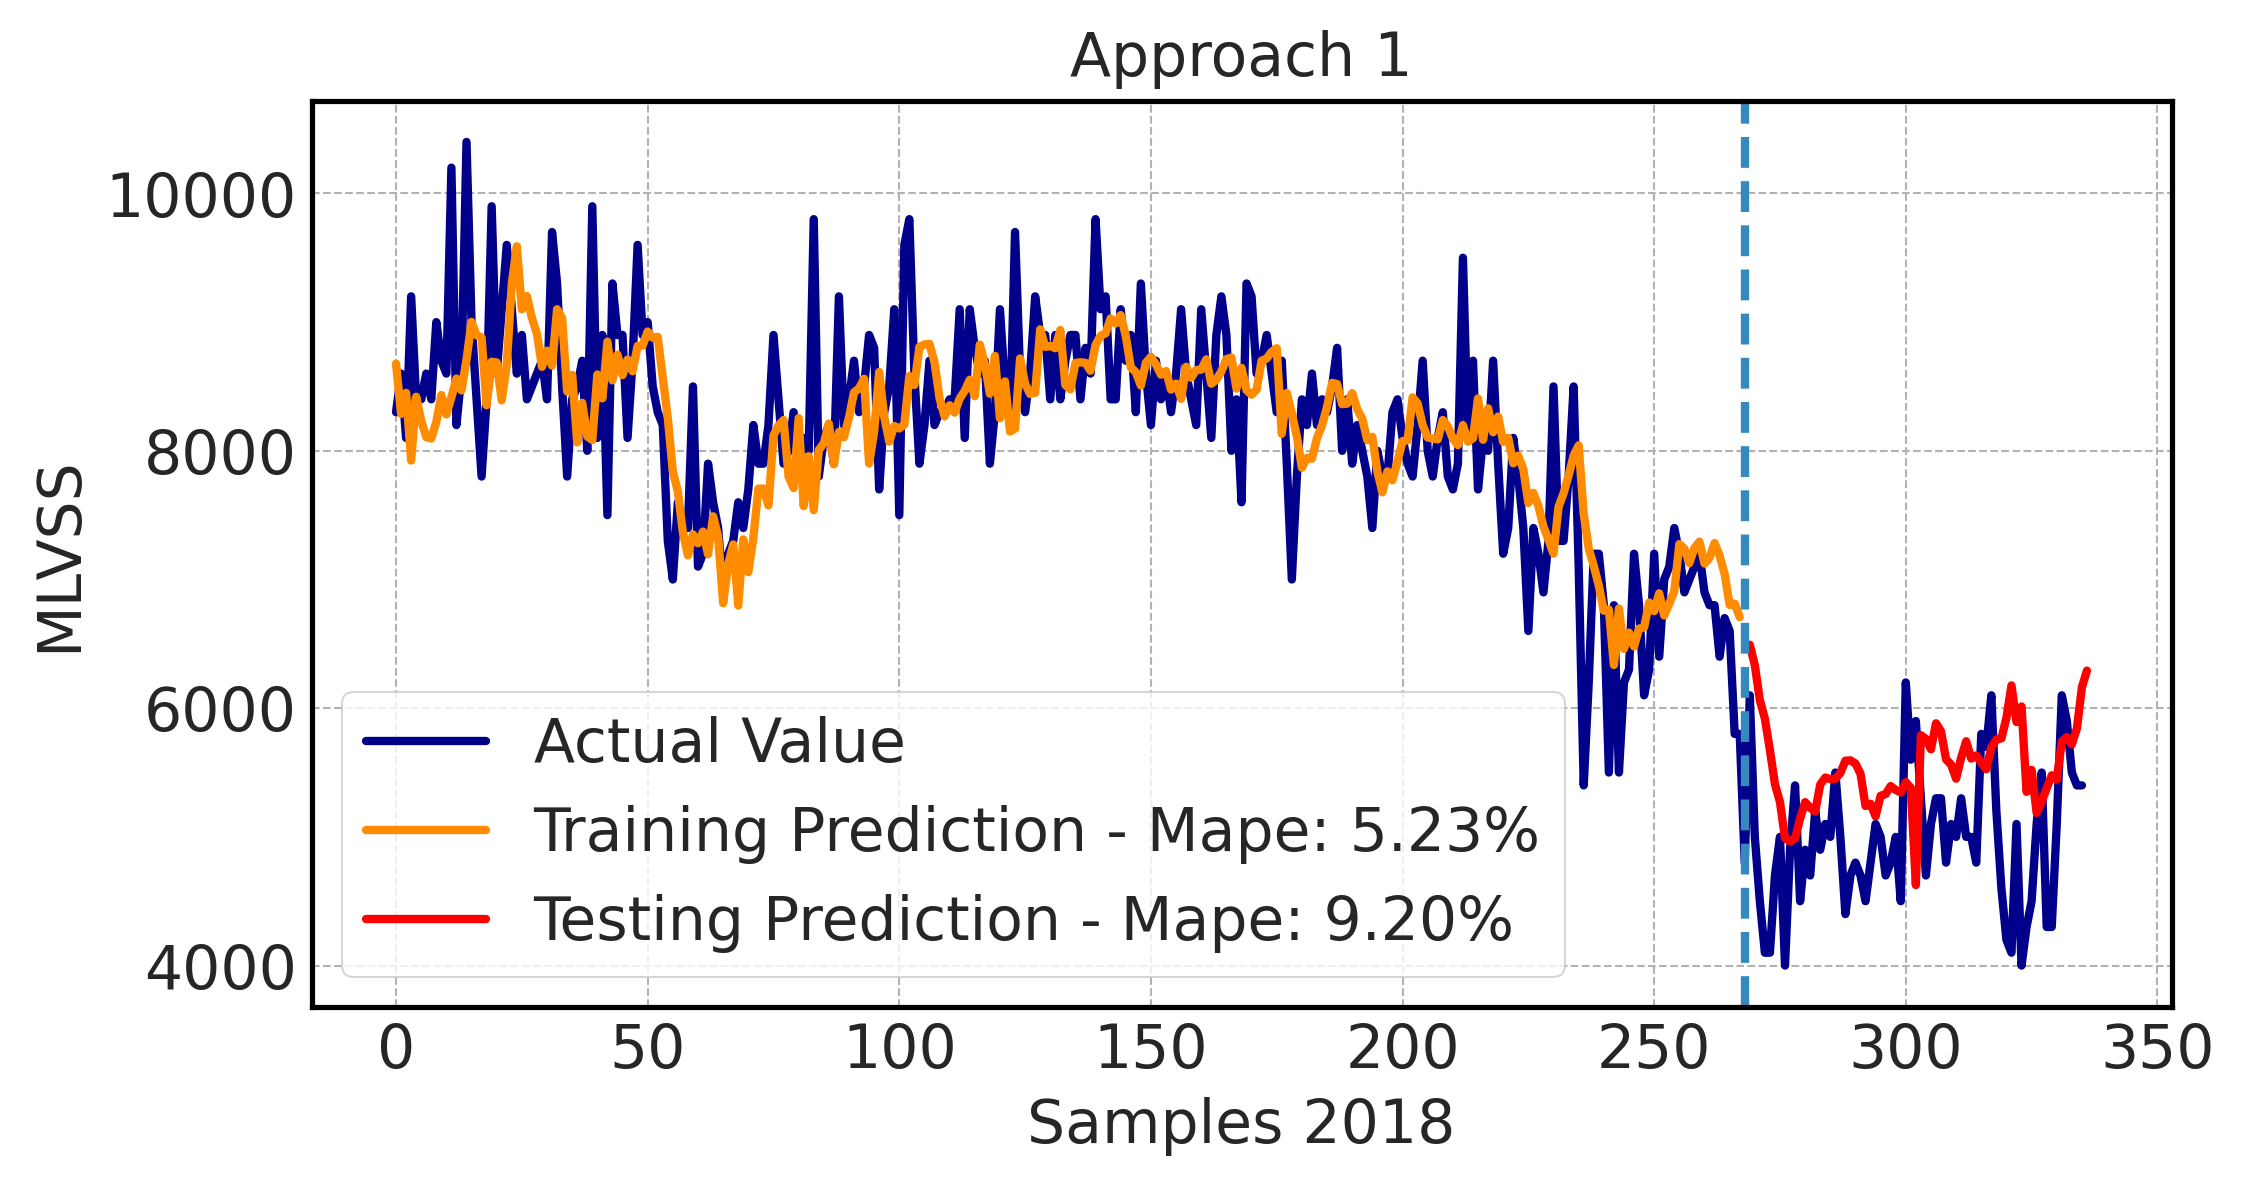
\includegraphics[width=\linewidth]{figures/Ch5/MVLSS-approach1.png}
\caption{Approach 1 - MLVSS}
\label{f:App1-MLVSS}
\end{figure}





\section{Approach 2}
The \ac{LSTM} architecture for each target variable and the approach prediction results are presented bellow. The \ac{LSTM} network implemented takes until 7 past days to predict one day a head.
All model hyper-parameters were tuned by a grid search within the following options:

\begin{itemize}
    \item Loss = [mse, mae]
    \item Optimizer = [SGD, adam]
    \item Activation = [Relu, linear, tanh]
    \item Number of Layers = [1, 2]
    \item Number of Neurons per layer = [2, 4, 6, 8, 10, 12, 14, 16, 18, 20, 22, 24, 26, 28, 30, 32]
    \item Batch Normalization = [0, 1]
    \item Dropout = [0, 1]
\end{itemize}

For Batch normalization and Dropout 0 means they are not included in the network.

\subsection{COD Discharge}
\autoref{f:App2-codd-nn} shows the structure of the \ac{LSTM} used for \ac{COD}\textsubscript{D} prediction which hyper-parameters are presented below. \autoref{f:App2-codd} shows the prediction results of this approach.

\begin{figure}[h]
\centering
 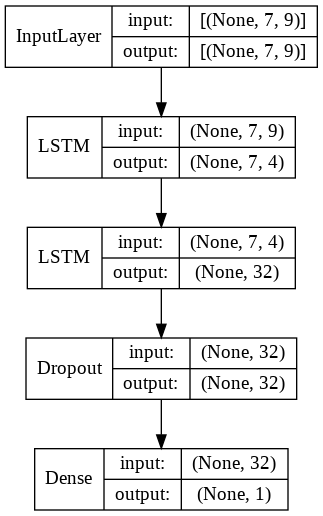
\includegraphics[width=0.4\linewidth]{figures/Ch5/App2_CODd.png}
\caption{Approach 2 - COD\textsubscript{D} LSTM Network}
\label{f:App2-codd-nn}
\end{figure}

\begin{figure}[h!]
\centering
\includegraphics[width=\linewidth]{figures/Ch5/CODd-2.png}
\caption{Approach 2 - COD\textsubscript{D}}
\label{f:App2-codd}
\end{figure}

\begin{itemize}
    \item Loss = mse
    \item Optimizer = SGD
    \item Activation =  Tanh
    \item Number of Layers = 2
    \item Number of Neurons per layer = [4, 32]
    \item Batch Normalization = 0
    \item Dropout = 1
\end{itemize}

\subsection{COD Equalizer}
\autoref{f:App2-codeq-nn} shows the structure of the \ac{LSTM} used for \ac{COD}\textsubscript{EQ} prediction which hyper-parameters are presented below. \autoref{f:App2-codeq} shows the prediction results of this approach.

\begin{itemize}
    \item Loss = mse
    \item Optimizer = Adam
    \item Activation =  Tanh
    \item Number of Layers = 2
    \item Number of Neurons per layer = [2, 18]
    \item Batch Normalization = 1
    \item Dropout = 0
\end{itemize}

\begin{figure}[h]
\centering
 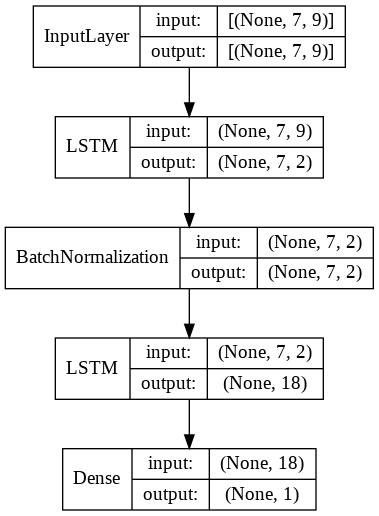
\includegraphics[width=0.4\linewidth]{figures/Ch5/App2_CODeq.png}
\caption{Approach 2 - COD\textsubscript{EQ} LSTM Network}
\label{f:App2-codeq-nn}
\end{figure}

\begin{figure}[h]
\centering
\includegraphics[width=\linewidth]{figures/Ch5/CODeq-2.png}
\caption{Approach 2 - COD\textsubscript{EQ}}
\label{f:App2-codeq}
\end{figure}

\subsection{MLVSS}
\autoref{f:App2-MLVSS-nn} shows the structure of the \ac{LSTM} used for \ac{MLVSS} prediction which hyper-parameters are presented below. \autoref{f:App2-MLVSS} shows the prediction results of this approach.

\begin{figure}[h]
\centering
 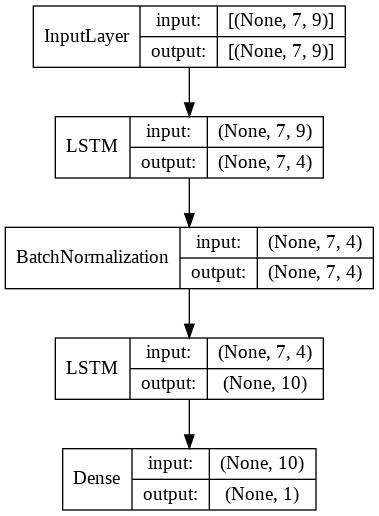
\includegraphics[width=0.4\linewidth]{figures/Ch5/App2_MLVSS.png}
\caption{Approach 2 - MLVSS LSTM Network}
\label{f:App2-MLVSS-nn}
\end{figure}

\begin{figure}[h]
\centering
\includegraphics[width=\linewidth]{figures/Ch5/MVLSS-approach2.png}
\caption{Approach 2 - MLVSS}
\label{f:App2-MLVSS}
\end{figure}

\begin{itemize}
    \item Loss = mse
    \item Optimizer = Adam
    \item Activation =  Linear
    \item Number of Layers = 2
    \item Number of Neurons per layer = [4, 10]
    \item Batch Normalization = 1
    \item Dropout = 0
\end{itemize}

%-----------------------------------------------
\section{Approach 3}

\begin{figure}[h!]
\centering
\includegraphics[width=\linewidth]{figures/Ch5/CODd-3.png}
\caption{Approach 3 - COD\textsubscript{D}}
\label{f:App3-codd}
\end{figure}

The last approach predicts using \ac{SVR} algorithm.

\begin{figure}[h!]
\centering
\includegraphics[width=\linewidth]{figures/Ch5/CODeq-3.png}
\caption{Approach 3 - COD\textsubscript{EQ}}
\label{f:App3-codeq}
\end{figure}

\begin{figure}[h!]
\centering
\includegraphics[width=\linewidth]{figures/Ch5/MVLSS-approach3.png}
\caption{Approach 3 - MLVSS}
\label{f:App3-MLVSS}
\end{figure}

This third model sometimes presents a shift prediction respect the expected value, nonetheless it achieves a good prediction. \autoref{f:App3-codd}, \autoref{f:App3-codeq}, and \autoref{f:App3-MLVSS} show the prediction results of this approach. 
\clearpage

%-----------------------------------------------
\section{Ensemble Approach 1 - Average}
The first ensemble approach makes an average of all three models presented before. \autoref{f:avg-codd}, \autoref{f:avg-codeq} and \autoref{f:avg-MLVSS} show the results of the average ensemble prediction for COD\textsubscript{D}, COD\textsubscript{EQ}, and MLVSS, respectively. 

\begin{figure}[h]
\centering
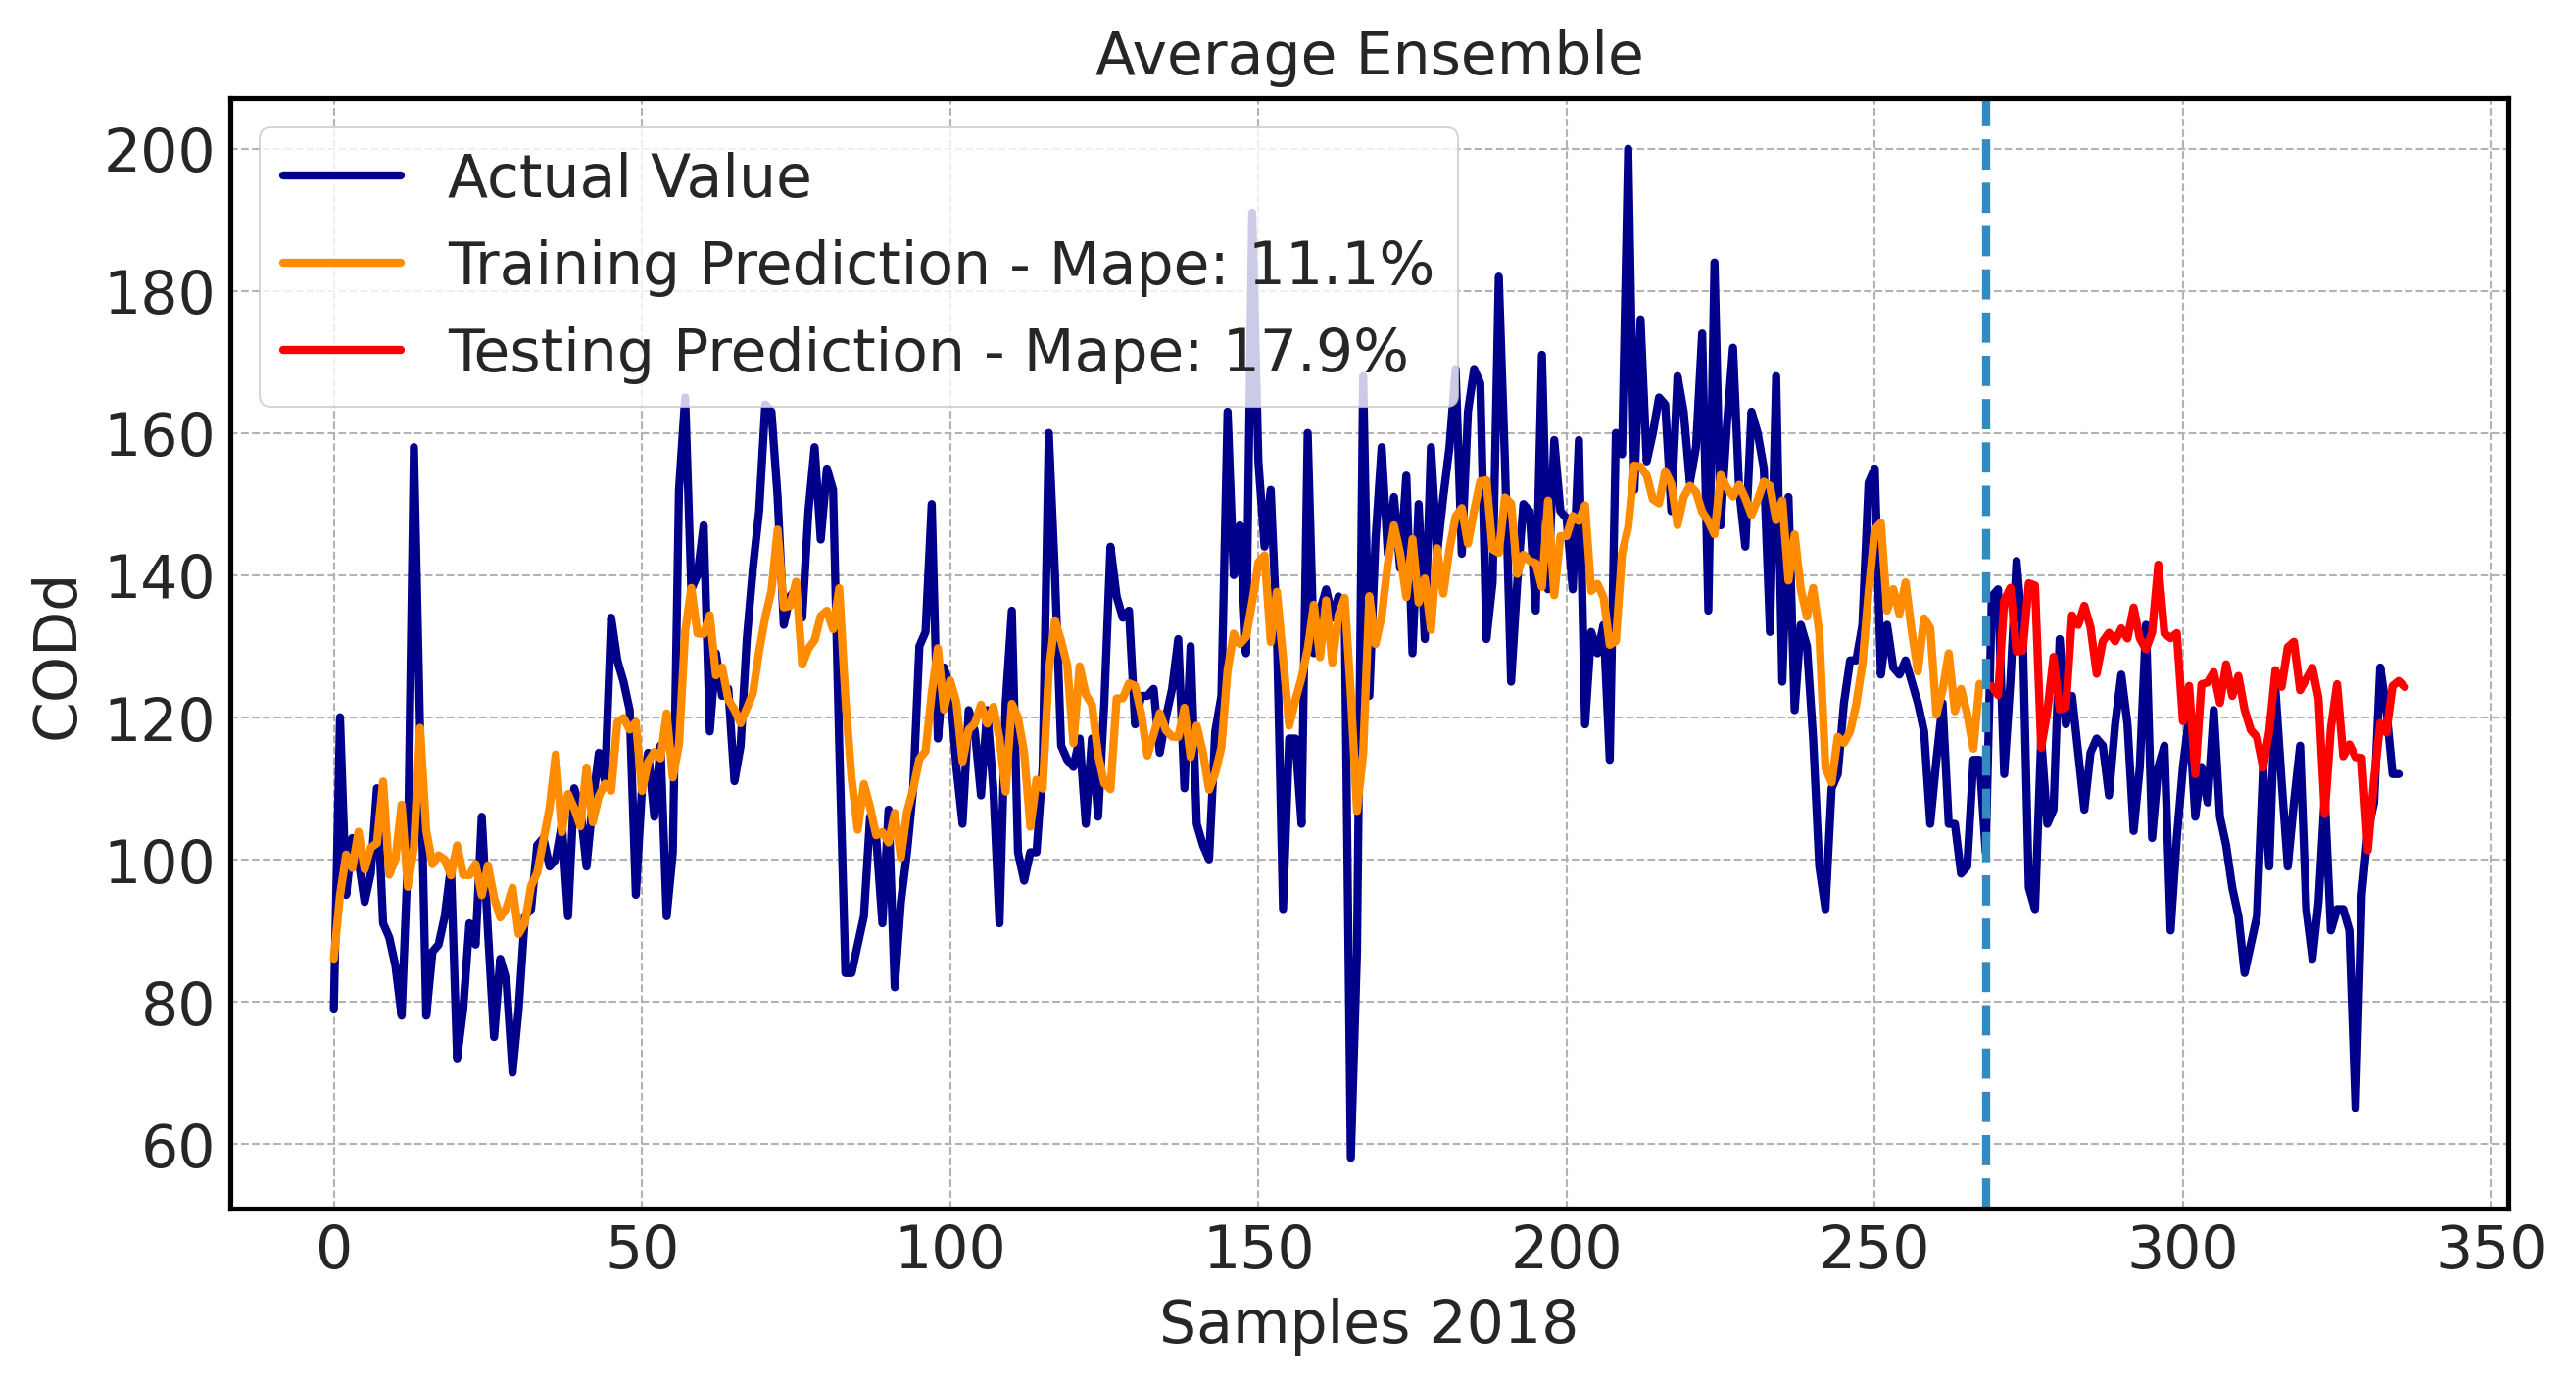
\includegraphics[width=\linewidth]{figures/Ch5/CODd-avg.png}
\caption{Average Ensemble - COD\textsubscript{D}}
\label{f:avg-codd}
\end{figure}

\begin{figure}[h]
\centering
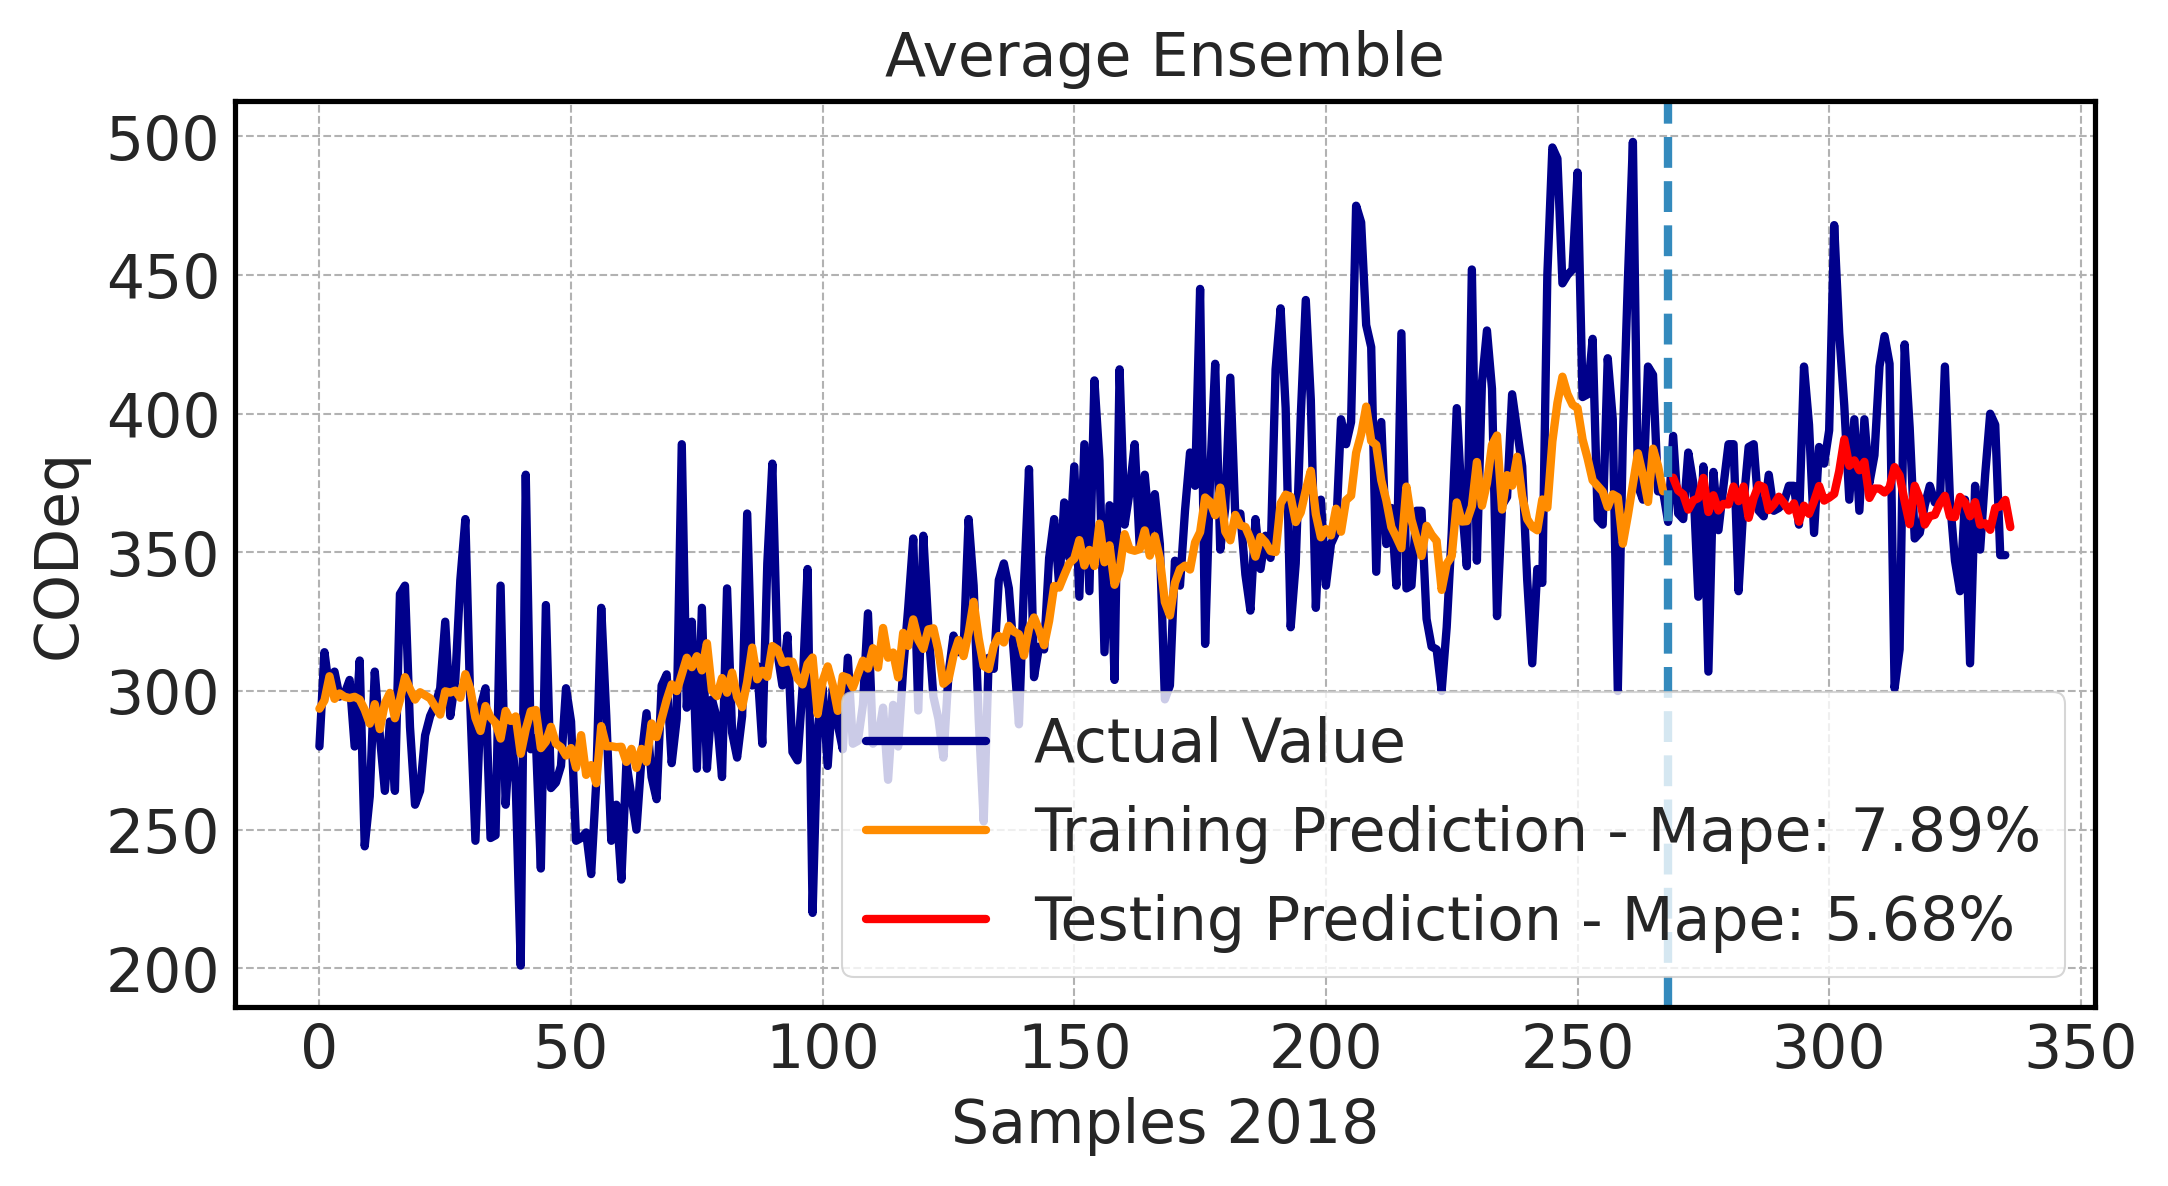
\includegraphics[width=\linewidth]{figures/Ch5/CODeq-avg.png}
\caption{Average Ensemble - COD\textsubscript{EQ}}
\label{f:avg-codeq}
\end{figure}

\begin{figure}[h]
\centering
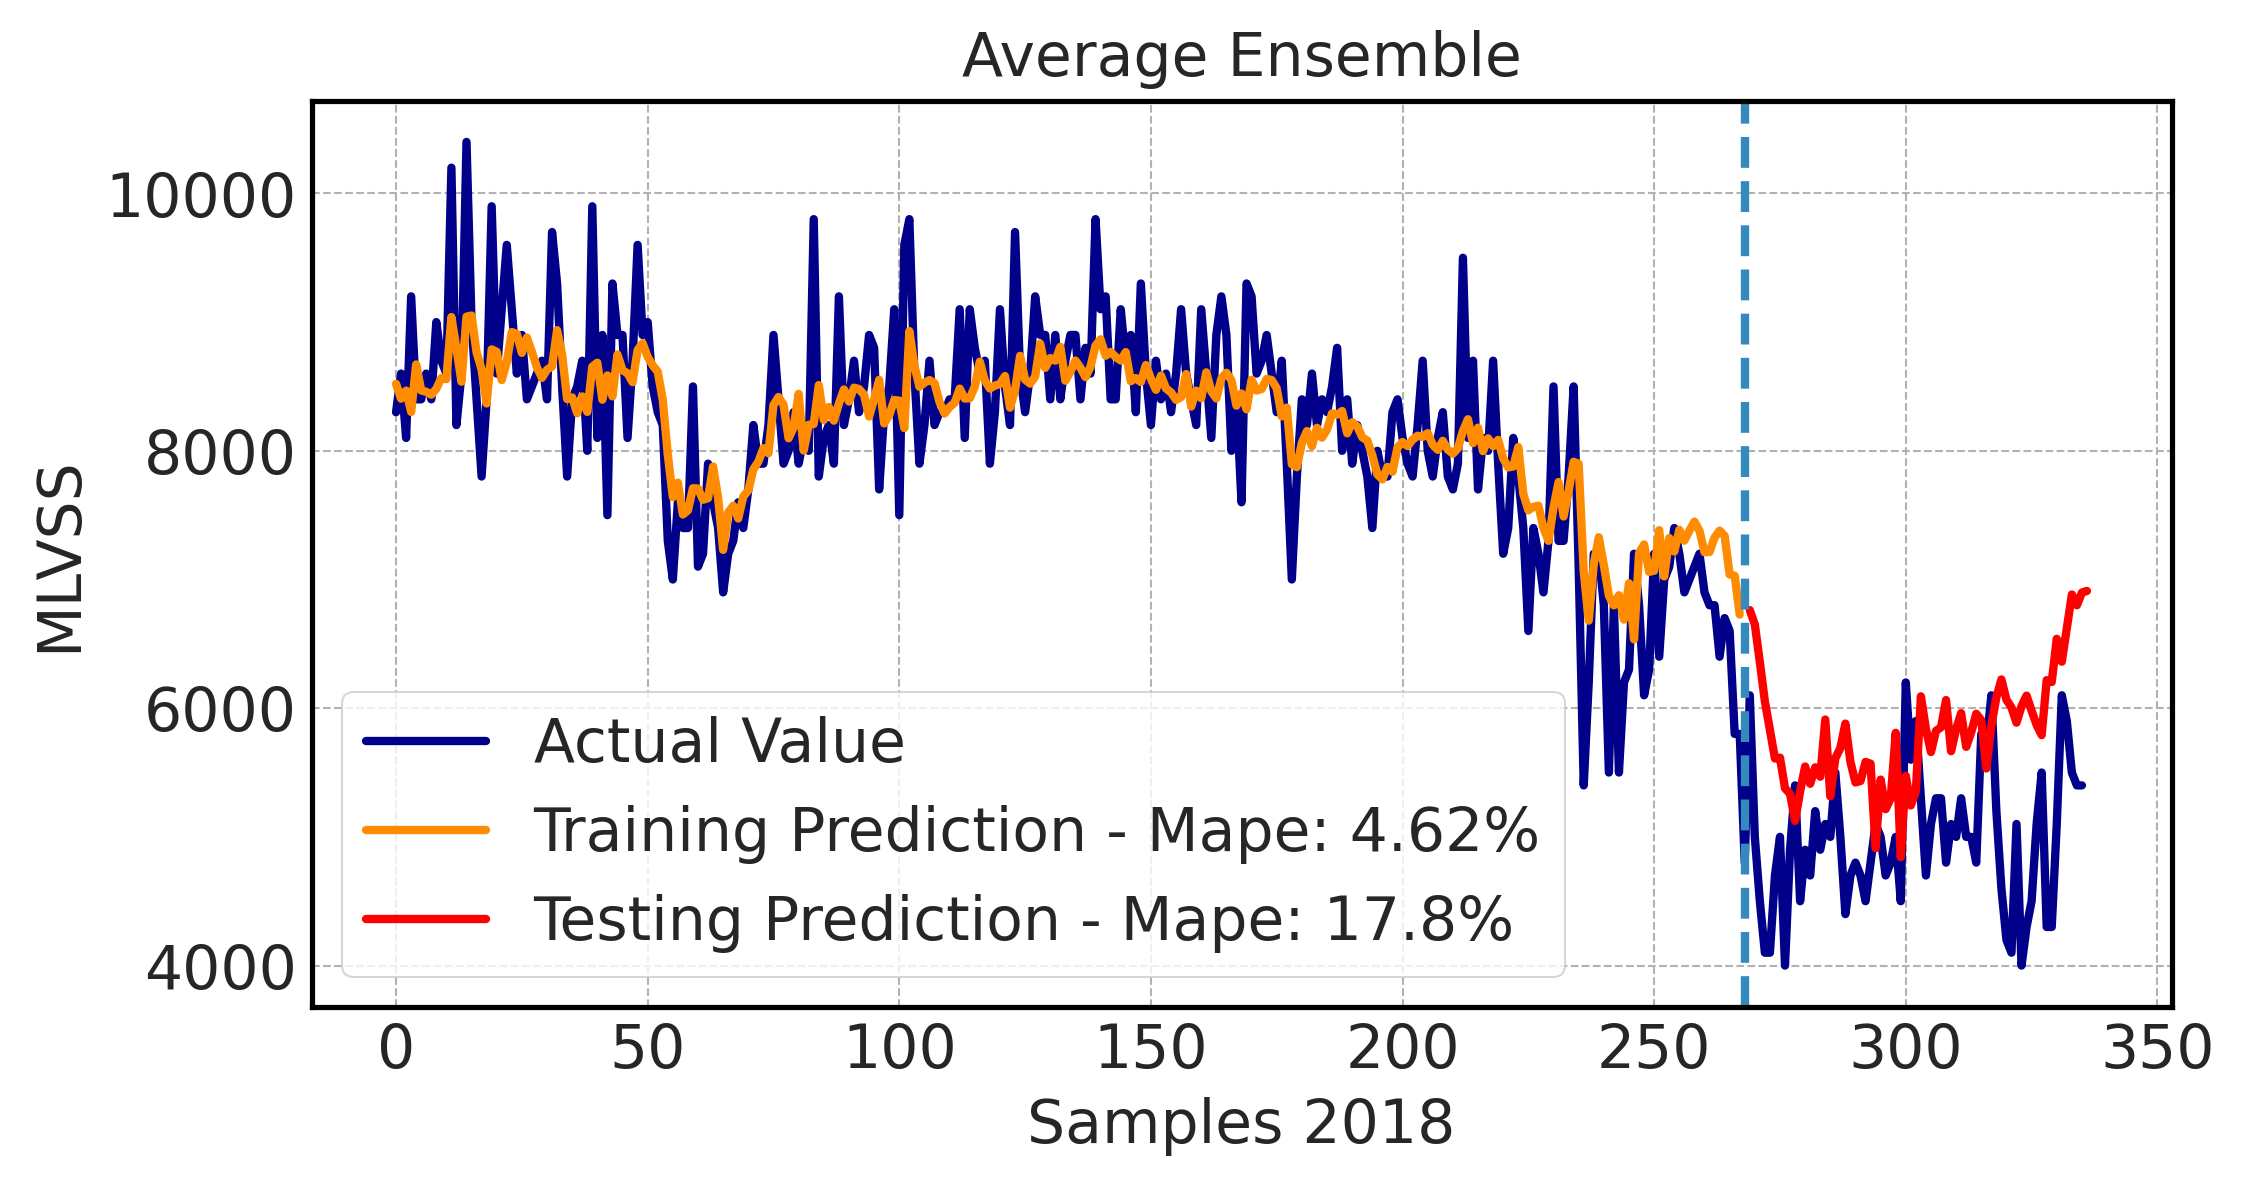
\includegraphics[width=\linewidth]{figures/Ch5/MVLSS-E_avg.png}
\caption{Average Ensemble - MLVSS}
\label{f:avg-MLVSS}
\end{figure}

%-----------------------------------------------
\section{Ensemble Approach 2 - MLP Fusion}
The second ensemble approach fuses all three models output presented before using a \ac{MLP}, and uses the exogenous variables as information source to enhance the final prediction. \autoref{f:avg-codd}, \autoref{f:avg-codeq} and \autoref{f:avg-MLVSS} show the results of the \ac{MLP} fusion ensemble prediction for the target variables. 

\begin{figure}[h]
\centering
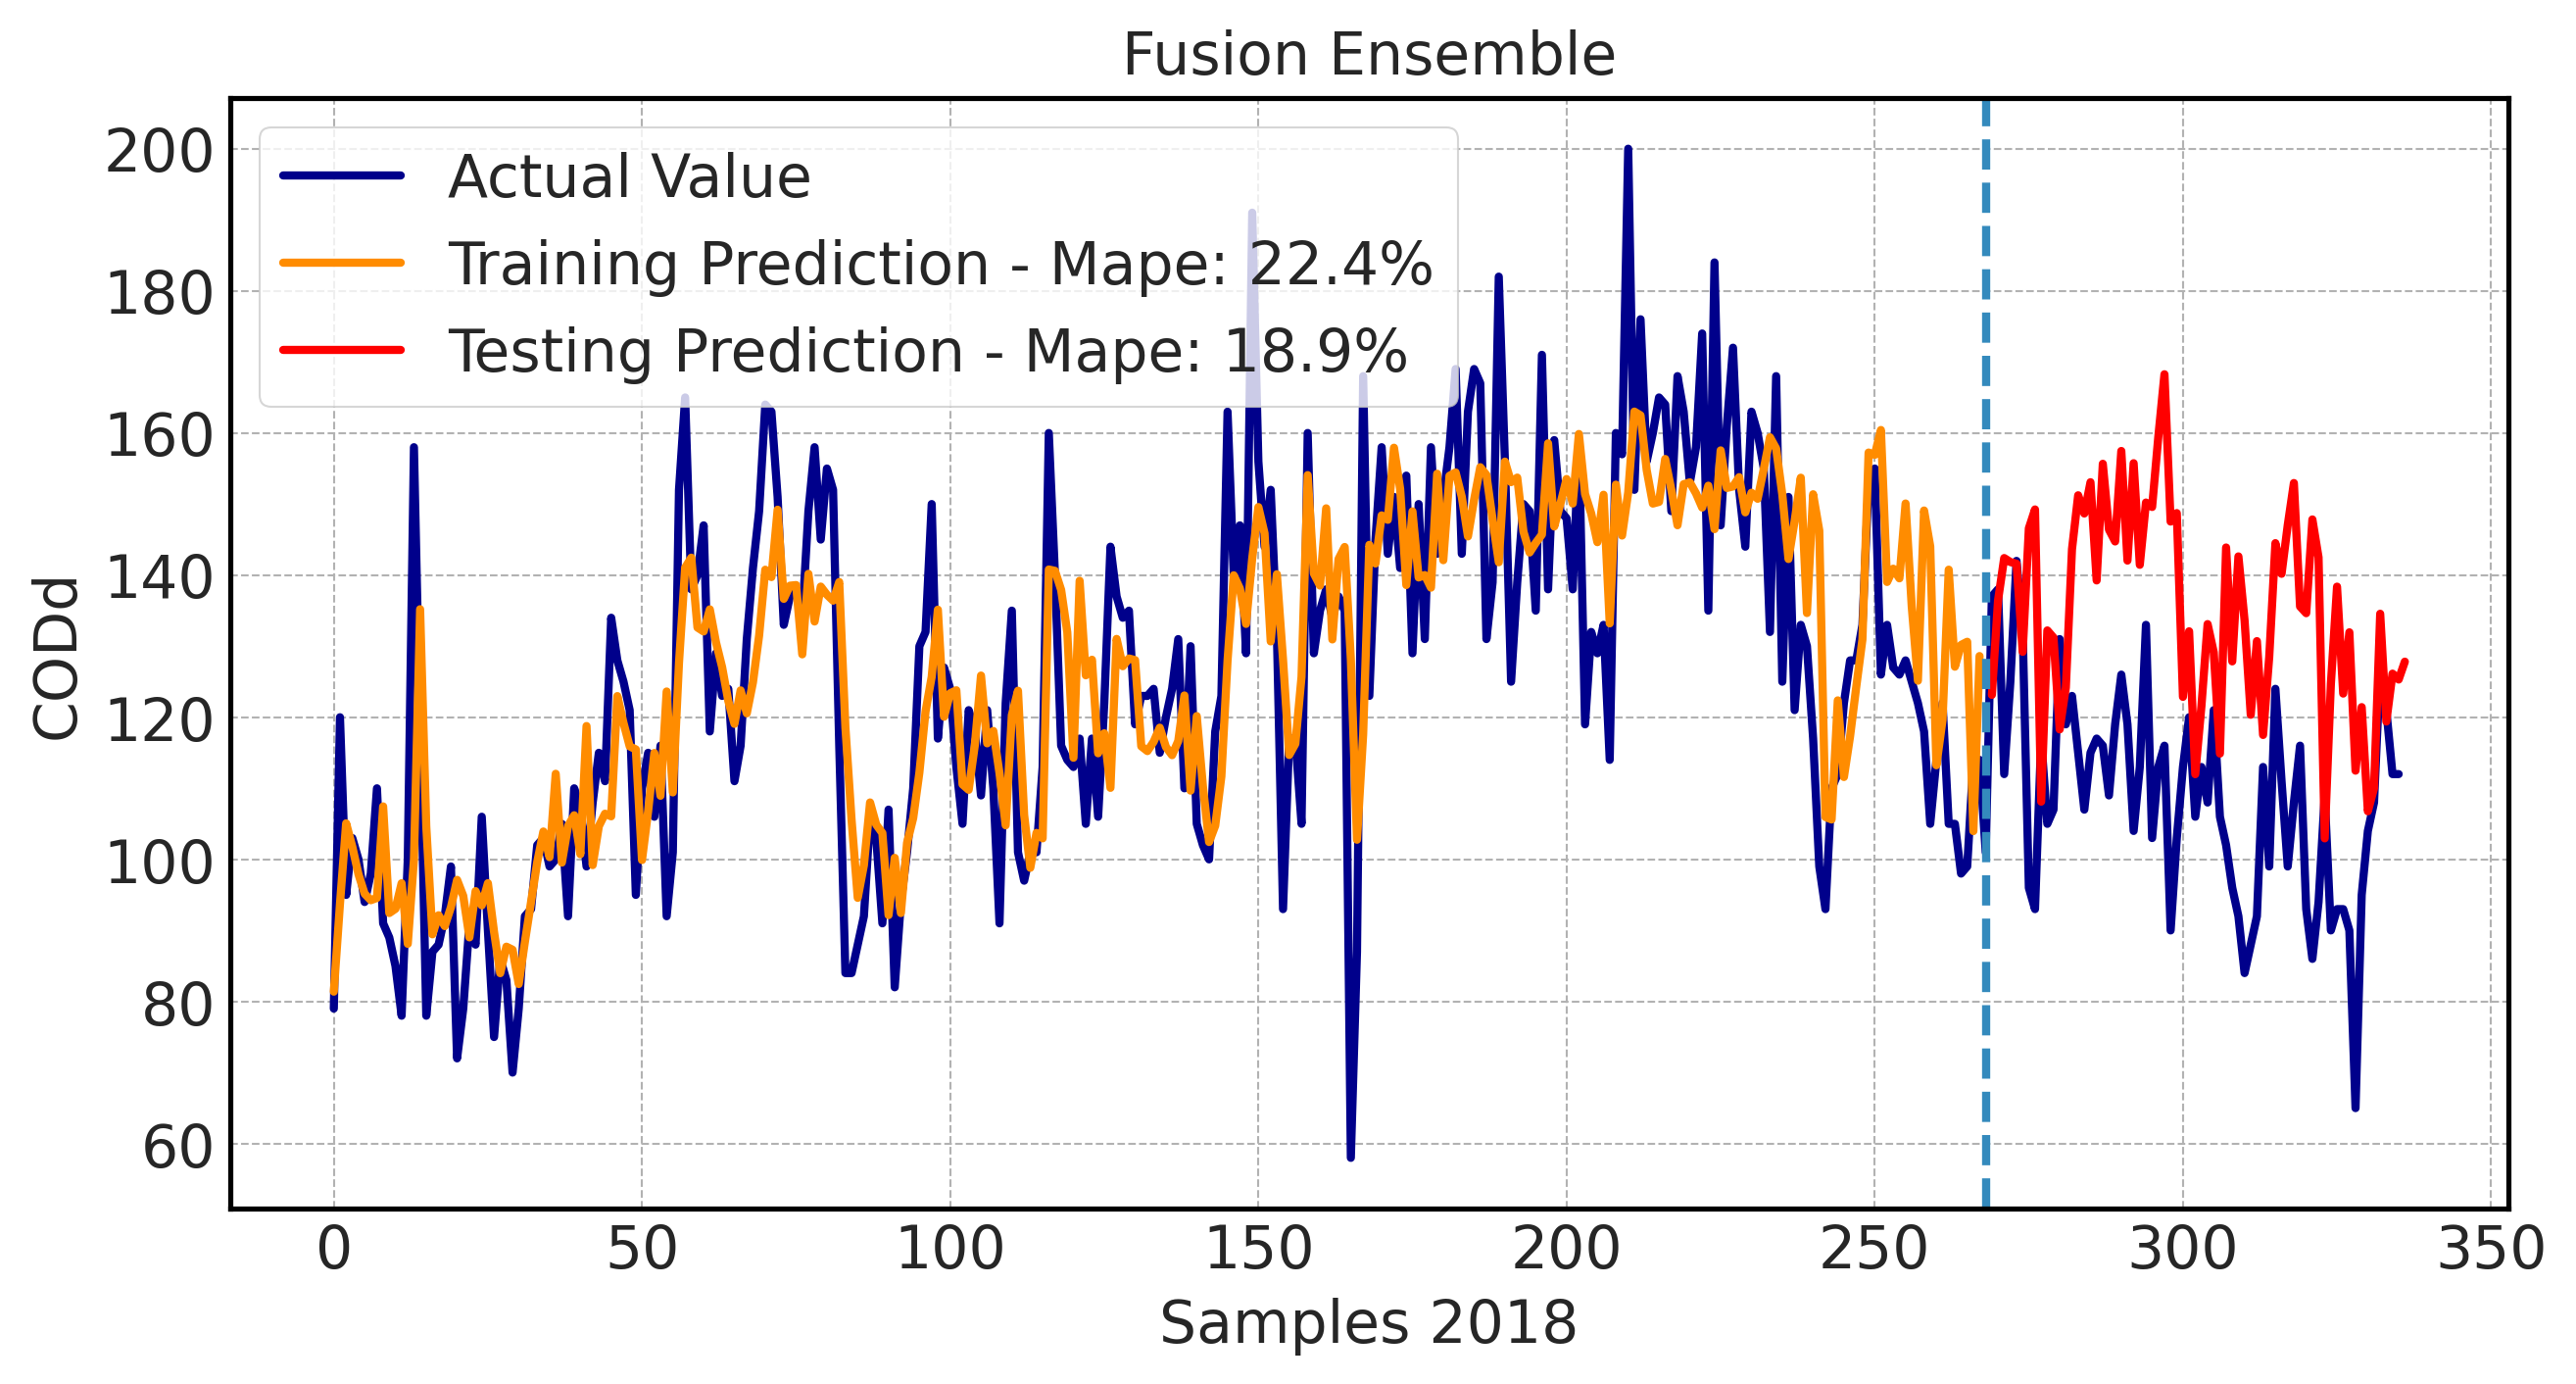
\includegraphics[width=\linewidth]{figures/Ch5/CODd-ann.png}
\caption{MLP Ensemble - COD\textsubscript{D}}
\label{f:ann-codd}
\end{figure}

\begin{figure}[h]
\centering
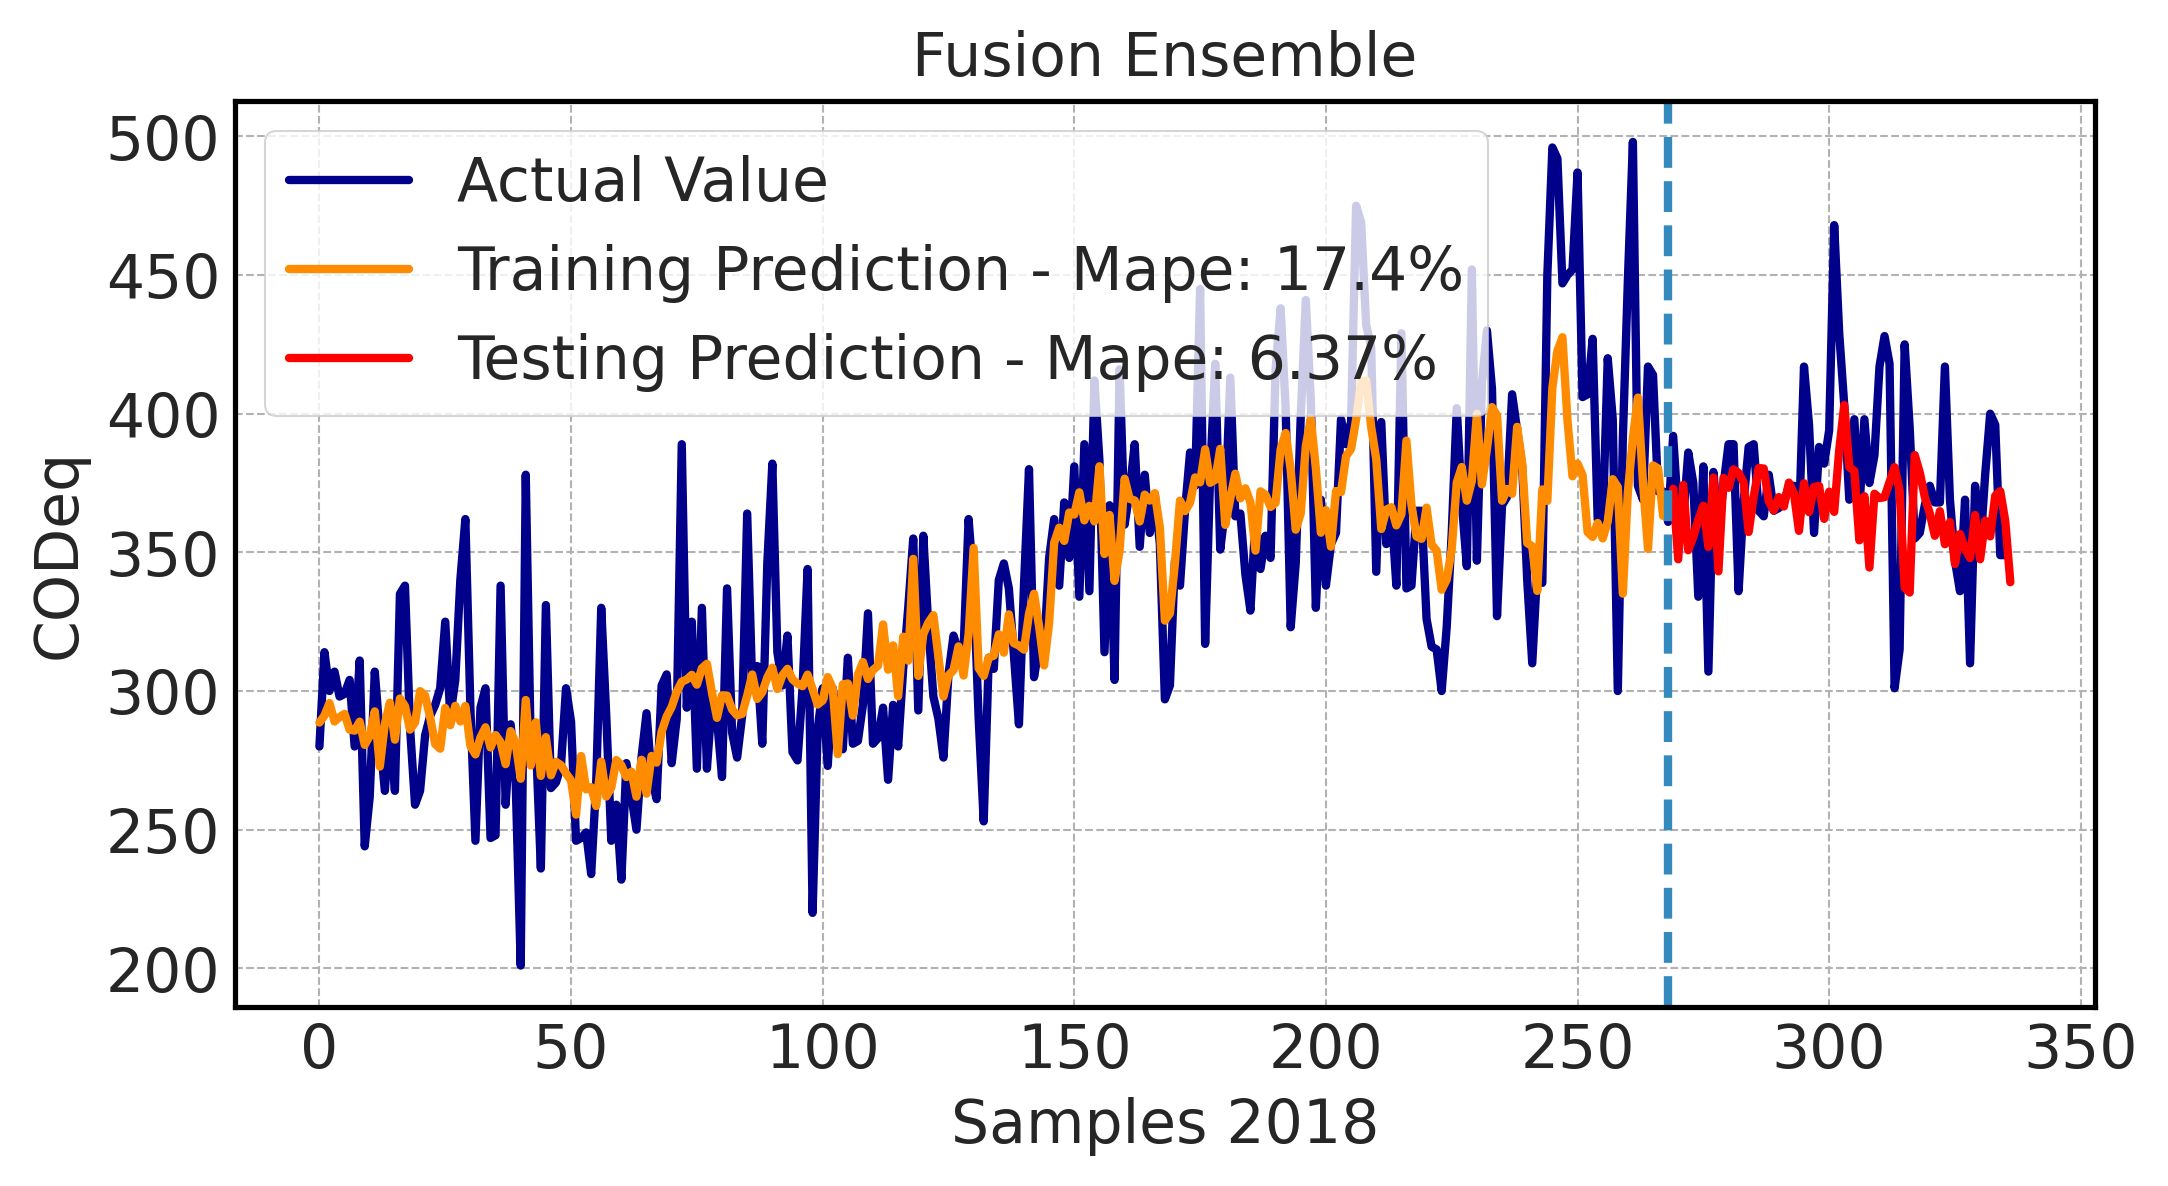
\includegraphics[width=\linewidth]{figures/Ch5/CODeq-ann.png}
\caption{MLP Ensemble - COD\textsubscript{EQ}}
\label{f:ann-codeq}
\end{figure}

\begin{figure}[h]
\centering
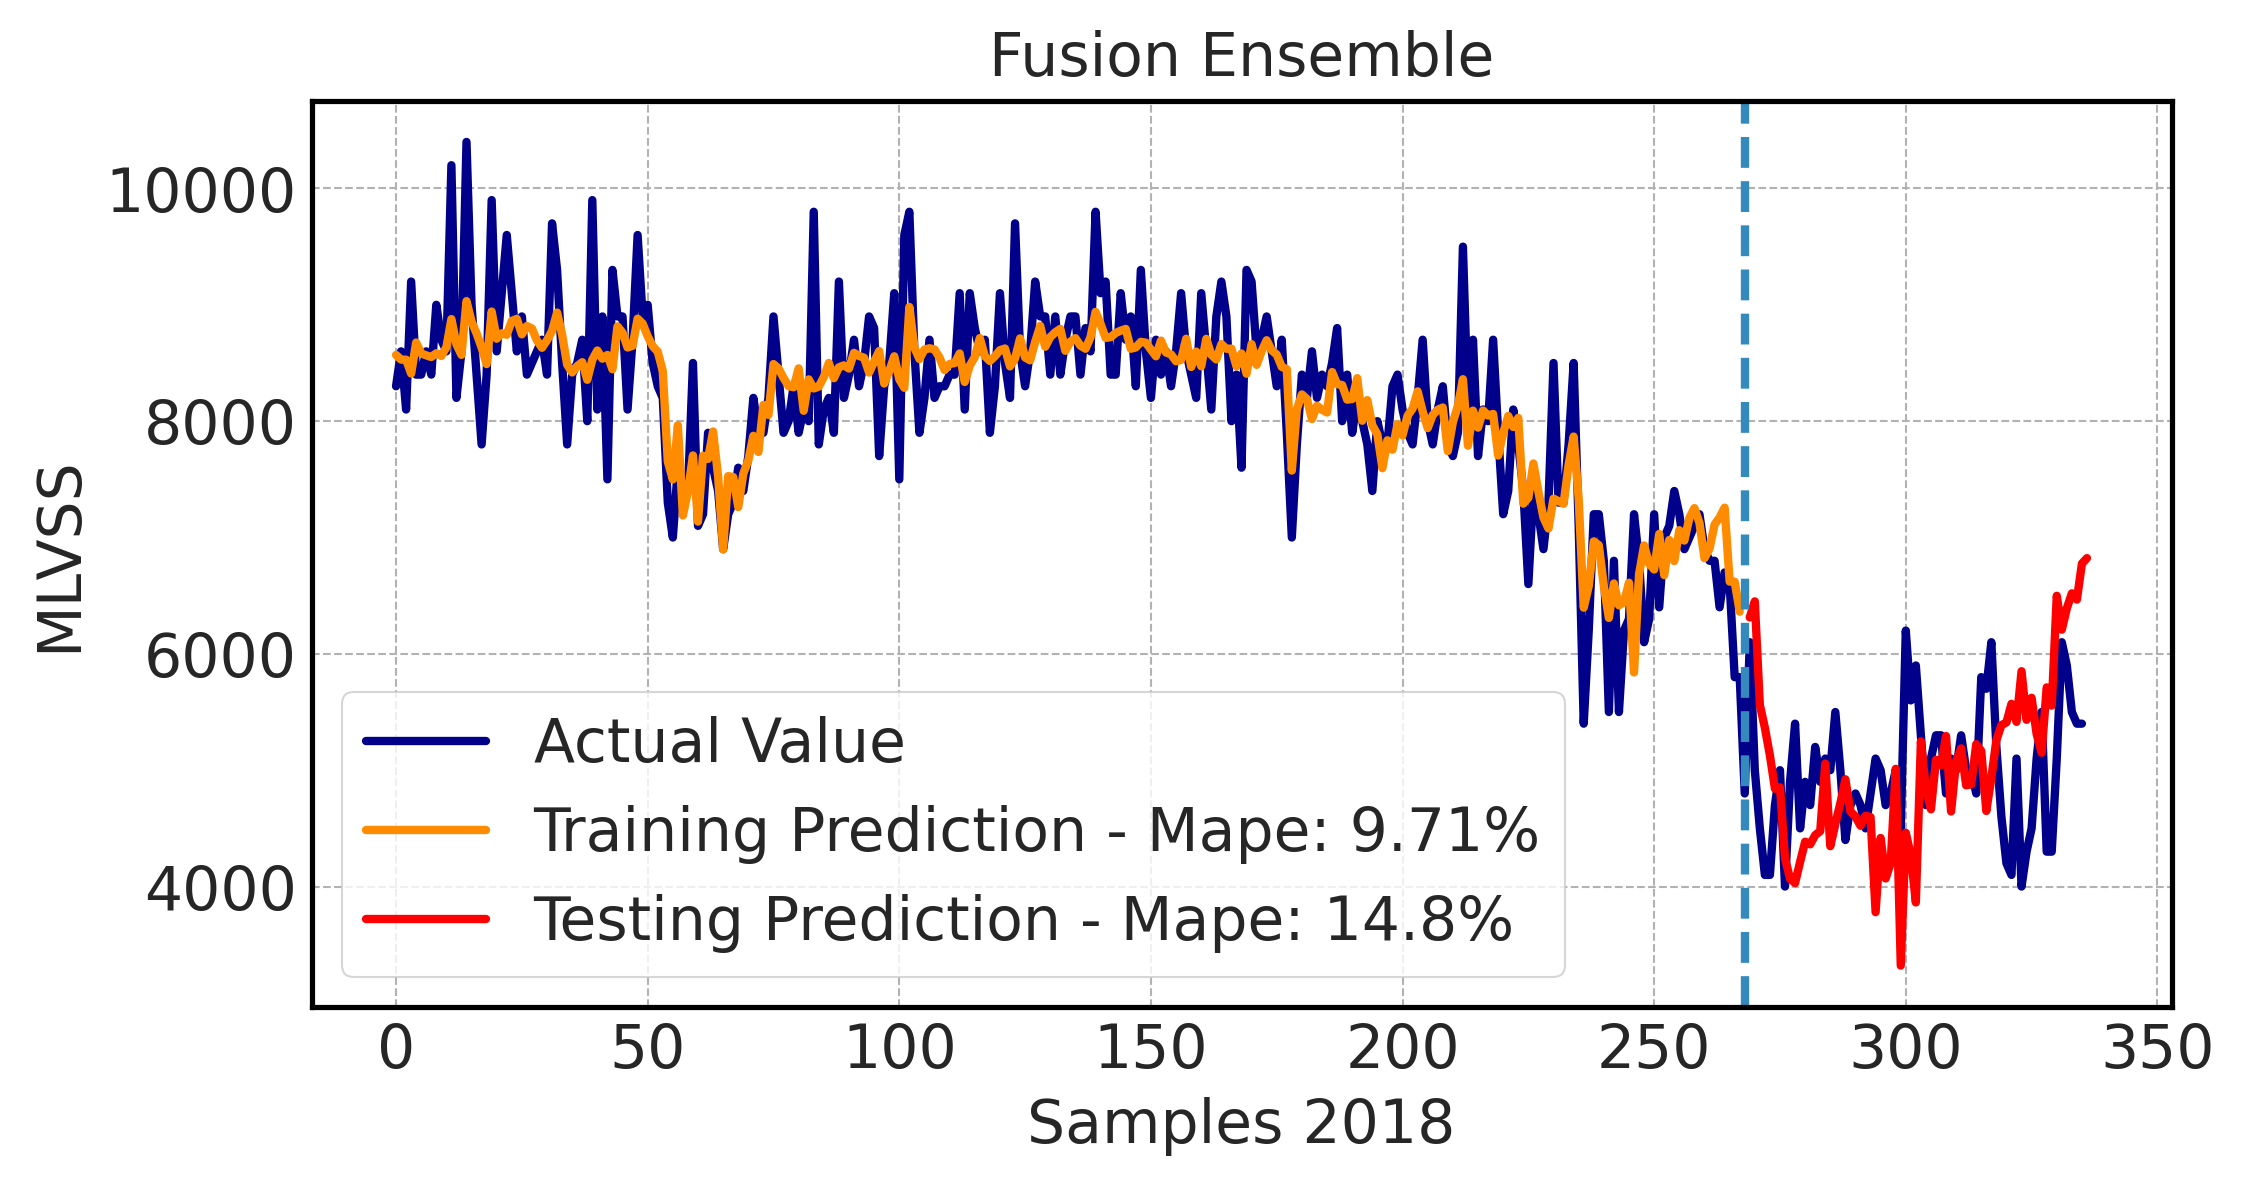
\includegraphics[width=\linewidth]{figures/Ch5/MVLSS-E_ann.png}
\caption{MLP Ensemble - MLVSS}
\label{f:ann-MLVSS}
\end{figure}

%-----------------------------------------------
\section{Ensemble Approach 3 - Selection}
The last ensemble approach predict which model will perform the best based on the process conditions which are represented by the exogenous variables. This prediction allows to select one of the single model as the most suitable one to carry out the prediction. \autoref{f:avg-codd}, \autoref{f:avg-codeq} and \autoref{f:avg-MLVSS} show the results of this ensemble approach prediction for the target variables. 

\begin{figure}[h!]
\centering
\includegraphics[width=\linewidth]{figures/Ch5/CODd-ann2.png}
\caption{MLP Ensemble - COD\textsubscript{D}}
\label{f:ann2-codd}
\end{figure}

\begin{figure}[h!]
\centering
\includegraphics[width=\linewidth]{figures/Ch5/CODeq-ann2.png}
\caption{MLP Ensemble - COD\textsubscript{EQ}}
\label{f:ann2-codeq}
\end{figure}

\begin{figure}[h!]
\centering
\includegraphics[width=\linewidth]{figures/Ch5/MVLSS-E_ann2.png}
\caption{MLP Ensemble - MLVSS}
\label{f:ann2-MLVSS}
\end{figure}

\section{Discussion}
\label{s:Contribution-2-Summary}

This chapter presents the implementation and obtained results of 3 approaches to predict time series variables of the wastewater treatment process. Also, 3 different ensemble approaches are presented in order to enhance the intelligent system prediction performance.
\autoref{t:Results} summarizes the \ac{MAPE} results obtained by the single models and the ensembles approaches. It is worth to mention that hyper-parameter tune was made using the training set as well as the evaluation of ensemble model enhancement. The best model performance over the training is highlighted in bold. The ensemble models offer a more robust prediction and present some improvements in \ac{MAPE}\%.
%\begin{longtable}{@{}l *{2}{rr}}
\begin{longtable}[h]{@{}l *{6}{rr}}
\caption[Approaches results]{Approaches results}
\label{t:Results}
\\
%   
\toprule%


 {\bfseries MAPE } & {\bfseries App.1} & ~ & {\bfseries App.2} & ~ & {\bfseries App.3} & ~ & {\bfseries Ens.1} & ~ & {\bfseries Ens.2} & ~ & {\bfseries Ens.3}
\\

\cmidrule[0.4pt](r{0.125em}){1-1}%
\cmidrule[0.4pt](lr{0.125em}){2-3}%
\cmidrule[0.4pt](lr{0.125em}){4-5}%
\cmidrule[0.4pt](lr{0.125em}){6-7}%
\cmidrule[0.4pt](lr{0.125em}){8-9}%
\cmidrule[0.4pt](lr{0.125em}){10-11}%
\cmidrule[0.4pt](lr{0.125em}){12-13}%


  \endfirsthead

\endhead


        (\%) & Train & Test & Train & Test & Train & Test & Train & Test & Train & Test & Train & Test  \\ 
        \hline
        MVLSS & 5.23 & 9.2 & 9.81 & 19.0 & 5.81 & 31.8 & 4.62 & 17.8 & 9.71 & 14.8 & \textbf{3.99} & 11.3  \\ 
        COD\textsubscript{EQ} & 8.6 & 6.21 & 16.1 & 7.59 & 8.49 & 5.67 & 7.89 & 5.68 & 17.4 & 6.37 & \textbf{7.2} & 6.94  \\ 
        COD\textsubscript{D} & 11.6 & 13.7 & 21.3 & 26.5 & 10.7 & 15.5 & 11.1 & 17.9 & 22.4 & 18.9 & \textbf{10.6} & 15.3  \\ 


\bottomrule

\end{longtable}


  \chapter{Experiments}\label{c:Experiments}
  \hinttext{!!!ACTION REQUIRED!!!}
\hinttext{The structure I defined is generic and will most likely have to be adapted. I suggest that you skim through the pages and then clear the files \texttt{text/ch2.tex} to \texttt{text/ch7.tex} before you start writing.}

This is just an example. You may want to restructure this chapter, or even integrate it into you contribution chapter. 

\section{Experiment Setup}
\label{s:Experiment-Setup}

Define the goal of the experiment. If you compare algorithms, define the metrics/techniques that you will use to compare them and why.


\subsection{Environment and System Setup}
\label{s:Experiment-Env}

Detail the properties of the environmental conditions of your experiment. What hardware did you use? What compiler?


\subsection{Implemented Algorithms}
\label{s:Experiment-Algo}

\hinttext{Now you need to outline the scope of the experiment. For example, by listing the algorithms that you have implemented:}

In this section, we list the algorithms that we have included in our experimental study.

\begin{description}
%  \item[Na\"{i}ve Space Folding] is the classic method that was originally proposed by \citeauthor{HerbertF:1965:Dune}~\cite{HerbertF:1965:Dune} to utilize the Holtzmann effect to fold space.
  
 % \item[Post-Butlerian Algorithm:] This approach uses the extended fold space theory as described by \citeauthor{HerbertB:2002:Butlerian-Jihad}~\cite{HerbertB:2002:Butlerian-Jihad}. It relies on infinite recursion and can currently only be implemented by beings with a heightened perception through massive infusion of \emph{Spice Melange}.

  \item[Ixian Inverse:] This is our new approach to fold space using an intelligent apparatus that implements the complete algorithm discussed in \autoref{s:Contribution-2-Major-2-Minor-2}.

\end{description}


\section{Results}
\label{s:Experiment-Results}

Use a somewhat expressive title for each experiment. This way you may easily reference them again in the summary.

\subsection{Short Distance Travel}
\label{s:Short-Distance-Experiment}

In this experiment we attempt to fold space from the planet Giedi~Prime\footnote{\url{https://en.wikipedia.org/wiki/Giedi_Prime}} to Arrakis\footnote{\url{https://en.wikipedia.org/wiki/Arrakis}}. [...]


\subsection{Long Distance Travel}
\label{s:Long-Distance-Experiment}

In this experiment we attempt to fold space from the planet Giedi~Prime to the imperial capital on Salusa~Secundus\footnote{\url{https://en.wikipedia.org/wiki/Salusa_Secundus}}. [...]


\section{Summary}
\label{s:Experiments-Summary}

Summarize the key findings of the experiments you conducted.

  
  \chapter{Conclusions}\label{c:Conclusions}
  The selection and characterization of the most significant variables of the wastewater treatment process have been carried out satisfactorily using correlation analysis, autocorrelations and decomposition of the time series. With these variables, an intelligent system based on artificial neural networks was developed to be capable of giving an adequate prediction of chemical oxygen demand, one of the most suitable variables to measure the level of pollutant load in the water and make decisions. The results show that the model presented a MAPE of 10.8\%, which supports its good performance according to historical data mentioned in [14], where the testing step ranged between 10\% and 13\%, predicting BOD, COD or TSS. Additionally, it is worth mentioning that this work presents as a novelty the use of time-series decomposition techniques to address the COD prediction and using an ANN, in comparison with the works presented in Section 2, whose summary can be seen in Table 2. This methodology can be useful to improve the prediction of some complex variables in which the ANNs do not have the desired performance. Finally, a platform was possible to design mainly to visualize available WWTP variables, monitor COD forecasting and consult the historical measurements. 

In search of constant improvement of the industrial wastewater treatment process, it is considered for future works to scale the prediction of the system to other key variables of the process, obtain a larger amount of data considering newly available measurements in the process and increase the scope of the prediction.


\noindent Optional: Talk about the general development of the respective field of research during your candidature. Talk about how this influenced your work.

\section{Major Contribution 1}

What are the major thoughts and findings discussed in this thesis with respect to \autoref{c:Contribution-1}? How does your research advance the current state-of-the-art? Make sure that you do NOT simply repeat the summary of that chapter.

\section{Major Contribution 2}

What are the major thoughts and findings discussed in this thesis with respect to \autoref{c:Contribution-2}? How does your research advance the current state-of-the-art? Make sure that you do NOT simply repeat the summary of that chapter.


\section{Outlook and Future Work}

Give an outlook regarding your expectations for the overall development of your chosen field of research. List topics that were not covered by your work. Identify and discuss potential avenues for follow-up research that you would consider worthwhile pursuing.
  
  \cleardoublepage

  % Bibliography
\label{app:Appendix} % Reference the bibliography elsewhere with \autoref{app:Bibliography}

\manualmark % Work-around to have small caps also here in the headline
\markboth{\spacedlowsmallcaps{Appendices}}{\spacedlowsmallcaps{Appendices}} % Work-around to have small caps also
%\phantomsection
\refstepcounter{dummy}


\addcontentsline{toc}{chapter}{\tocEntry{Appendices}}
 %Add appendices title to toc
  \appendix
 \chapter{Appendix 1}\label{app:A}
  \acresetall 
  \input{text/app-a}
  \acresetall 
  \chapter{Appendix 2}\label{app:B}
  \input{text/app-b}

  
  \singlespacing
  % Bibliography
\label{app:Bibliography} % Reference the bibliography elsewhere with \autoref{app:Bibliography}

\manualmark % Work-around to have small caps also here in the headline
\markboth{\spacedlowsmallcaps{\bibname}}{\spacedlowsmallcaps{\bibname}} % Work-around to have small caps also
%\phantomsection
\refstepcounter{dummy}

\addtocontents{toc}{\protect\vspace{\beforebibskip}} % Place the bibliography slightly below the rest of the document content in the table of contents
\addcontentsline{toc}{chapter}{\tocEntry{\bibname}}
\printbibliography
  \cleardoublepage
  
  \pagestyle{empty}
  \onehalfspacing
  \hfill
\vfill
\section*{Colophon}

\hinttext{This page is entirely optional. However, credit should be given where it is due. Please make sure that you attribute the work of others appropriately.}

This document was authored using \texttt{TeXstudio}\footnote{\url{https://www.texstudio.org}} and typeset based on the \texttt{La Trobe PhD Thesis Template}\footnote{\url{https://github.com/bashimao/ltu-thesis}} (customization of the \texttt{classicthesis}\footnote{\url{https://bitbucket.org/amiede/classicthesis}} \LaTeX{} template) using \texttt{TeX~Live}\footnote{\url{https://tug.org/texlive}} on a machine running \texttt{LinuxMint}\footnote{\url{https://linuxmint.com}}. Other notable software tools used during the production of this document:
\texttt{GNU~Octave}\footnote{\url{https://www.gnu.org/software/octave}} and \texttt{LibreOffice}\footnote{\url{https://www.libreoffice.org}} for number crunching; \texttt{GIMP}\footnote{\url{https://www.gimp.org}} and \texttt{Inkscape}\footnote{\url{https://inkscape.org}} for working with graphics; \texttt{Mendeley Desktop}\footnote{\url{https://www.mendeley.com}} for reference management.\\

\bigskip


\end{document}